% !Mode:: "TeX:UTF-8"

\def\usewhat{pdflatex}                               % 定义编译方式 dvipdfmx 或者 pdflatex,默认为 dvipdfmx
                                                     % 方式编译,如果需要修改,只需改变花括号中的内容即可。
\documentclass[12pt,openany,oneside,ctexartutf8]{book}
                                                     % 本科生毕业论文通常采用单页排版
% !Mode:: "TeX:UTF-8"
%  Authors: 张井   Jing Zhang: prayever@gmail.com     天津大学2010级管理与经济学部信息管理与信息系统专业硕士生
%           余蓝涛 Lantao Yu: lantaoyu1991@gmail.com  天津大学2008级精密仪器与光电子工程学院测控技术与仪器专业本科生

%%%%%%%%%% Package %%%%%%%%%%%%
\usepackage{graphicx}                       % 支持插图处理
% \usepackage[a4paper,text={146.4true mm,239.2 true mm},top= 25.4true mm, bottom= 25.4true mm, left=31.7 true mm,head=6true mm,headsep=6.5true mm,foot=16.5true mm]{geometry}
\usepackage[a4paper,top=25.4mm, bottom=25.4mm, left=31.7mm, right=31.7mm, head=6true mm,headsep=6.5true mm,foot=17.5mm]{geometry}
                                            % 支持版面尺寸设置
\usepackage[squaren]{SIunits}               % 支持国际标准单位
 
\usepackage{titlesec}                       % 控制标题的宏包
\usepackage{titletoc}                       % 控制目录的宏包
\usepackage{fancyhdr}                       % fancyhdr宏包 支持页眉和页脚的相关定义
\usepackage[UTF8]{ctex}                     % 支持中文显示
\usepackage{CJKpunct}
\usepackage{color}                          % 支持彩色
\usepackage{amsmath}                        % AMSLaTeX宏包 用来排出更加漂亮的公式
\usepackage{amssymb}                        % 数学符号生成命令
\usepackage[below]{placeins}    %允许上一个section的浮动图形出现在下一个section的开始部分,还提供\FloatBarrier命令,使所有未处理的浮动图形立即被处理
\usepackage{multirow}                       % 使用Multirow宏包,使得表格可以合并多个row格
\usepackage{booktabs}                       % 表格,横的粗线;\specialrule{1pt}{0pt}{0pt}
\usepackage{longtable}                      % 支持跨页的表格。
\usepackage{tabularx}                       % 自动设置表格的列宽
\usepackage{subfigure}                      % 支持子图 %centerlast 设置最后一行是否居中
\usepackage[subfigure]{ccaption}            % 支持子图的中文标题
\usepackage[sort&compress,numbers]{natbib}  % 支持引用缩写的宏包
\usepackage{enumitem}                       % 使用enumitem宏包,改变列表项的格式
\usepackage{calc}                           % 长度可以用+ - * / 进行计算
\usepackage{txfonts}                        % 字体宏包
\usepackage{bm}                             % 处理数学公式中的黑斜体的宏包
\usepackage[amsmath,thmmarks,hyperref]{ntheorem}  % 定理类环境宏包,其中 amsmath 选项用来兼容 AMS LaTeX 的宏包
\usepackage{CJKnumb}                        % 提供将阿拉伯数字转换成中文数字的命令
\usepackage{indentfirst}                    % 首行缩进宏包
\usepackage{CJKutf8}                        % 用在UTF8编码环境下,它可以自动调用CJK,同时针对UTF8编码作了设置

% \usepackage{fancybox} 

%\usepackage{hypbmsec}                      % 用来控制书签中标题显示内容
\newcommand{\tabincell}[2]{\begin{tabular}{@{}#1@{}}#2\end{tabular}}
\usepackage{xcolor}
%支持代码环境
\usepackage{listings}
\lstset{numbers=left,
language=[ANSI]{C},
numberstyle=\tiny,
extendedchars=false,
showstringspaces=false,
breakatwhitespace=false,
breaklines=true,
captionpos=b,
keywordstyle=\color{blue!70},
commentstyle=\color{red!50!green!50!blue!50},
frame=shadowbox,
rulesepcolor=\color{red!20!green!20!blue!20}
}
%支持算法环境
\usepackage[boxed,ruled,lined]{algorithm2e}
\usepackage{algorithmic}

\usepackage{array}
\newcommand{\PreserveBackslash}[1]{\let\temp=\\#1\let\\=\temp}
\newcolumntype{C}[1]{>{\PreserveBackslash\centering}p{#1}}
\newcolumntype{R}[1]{>{\PreserveBackslash\raggedleft}p{#1}}
\newcolumntype{L}[1]{>{\PreserveBackslash\raggedright}p{#1}}

% 生成有书签的 pdf 及其生成方式。通常可以在 tjumain.tex 文件的第一行选择 pdflatex 或者是 dvipdfmx 编译手段。如果选择前者,则使用 pdflatex + pdflatex 编译; 如果选择后者,在编译的时候选择 latex + bibtex + latex + latex 编译。出现混淆的时候,系统会报错。
% 如果您的pdf制作中文书签有乱码使用如下命令,就可以解决了
\def\atemp{pdflatex}\ifx\atemp\usewhat
\usepackage{cmap}                           % pdflatex 编译时,可以生成可复制、粘贴的中文 PDF 文档, 缺点是在Windows上显示时效果不大好,字体发虚
\usepackage{hyperref}
\hypersetup{
    unicode,
    pdfborder={0 0 0},
}
\fi
% \usepackage[pdftex,unicode,
%             CJKbookmarks=true,
%             bookmarksnumbered=true,
%             bookmarksopen=true,
%             colorlinks=false,
%             pdfborder={0 0 0},
%             citecolor=blue,
%             linkcolor=red,
%             anchorcolor=green,
%             urlcolor=blue,
%             breaklinks=true
%             ]{hyperref}

                                % 定义本文所使用宏包
\graphicspath{{figures/}}                            % 定义所有的 .eps 文件在 figures 子目录下
\begin{document}                                     % 开始全文
\begin{CJK*}{UTF8}{song}                             % 开始中文字体使用
	% !Mode:: "TeX:UTF-8"
%  Authors: 张井   Jing Zhang: prayever@gmail.com     天津大学2010级管理与经济学部信息管理与信息系统专业硕士生
%           余蓝涛 Lantao Yu: lantaoyu1991@gmail.com  天津大学2008级精密仪器与光电子工程学院测控技术与仪器专业本科生

% 2018/5/23修正
%           李幼萌 Youmeng Li: liyoumeng@tju.edu.cn   天津大学软件学院软件工程系

%%%%%%%%%%%%%%%%% Fonts Definition and Basics %%%%%%%%%%%%%%%%%
\newcommand{\song}{\CJKfamily{song}}    % 宋体
\newcommand{\fs}{\CJKfamily{fs}}        % 仿宋体
\newcommand{\kai}{\CJKfamily{kai}}      % 楷体
\newcommand{\hei}{\CJKfamily{hei}}      % 黑体
\newcommand{\li}{\CJKfamily{li}}        % 隶书
\newcommand{\yihao}{\fontsize{26pt}{26pt}\selectfont}       % 一号, 单倍行距
\newcommand{\xiaoyi}{\fontsize{24pt}{24pt}\selectfont}      % 小一, 单倍行距
\newcommand{\erhao}{\fontsize{22pt}{1.25\baselineskip}\selectfont}       % 二号, 1.25倍行距
\newcommand{\xiaoer}{\fontsize{18pt}{18pt}\selectfont}      % 小二, 单倍行距
\newcommand{\sanhao}{\fontsize{16pt}{16pt}\selectfont}      % 三号, 单倍行距
\newcommand{\xiaosan}{\fontsize{15pt}{15pt}\selectfont}     % 小三, 单倍行距
\newcommand{\sihao}{\fontsize{14pt}{14pt}\selectfont}       % 四号, 单倍行距
\newcommand{\xiaosi}{\fontsize{12pt}{12pt}\selectfont}      % 小四, 单倍行距
\newcommand{\wuhao}{\fontsize{10.5pt}{10.5pt}\selectfont}   % 五号, 单倍行距
\newcommand{\xiaowu}{\fontsize{9pt}{9pt}\selectfont}        % 小五, 单倍行距

\CJKtilde  % 重新定义了波浪符~的意义
\newcommand\prechaptername{第}
\newcommand\postchaptername{章}

\punctstyle{hangmobanjiao}             % 调整中文字符的表示,行内占一个字符宽度,行尾占半个字符宽度

% 调整罗列环境的布局
\setitemize{leftmargin=3em,itemsep=0em,partopsep=0em,parsep=0em,topsep=-0em}
\setenumerate{leftmargin=3em,itemsep=0em,partopsep=0em,parsep=0em,topsep=0em}

% 避免宏包 hyperref 和 arydshln 不兼容带来的目录链接失效的问题。
\def\temp{\relax}
\let\temp\addcontentsline
\gdef\addcontentsline{\phantomsection\temp}

% 自定义项目列表标签及格式 \begin{publist} 列表项 \end{publist}
\newcounter{pubctr} %自定义新计数器
\newenvironment{publist}{%%%%%定义新环境
\begin{list}{[\arabic{pubctr}]} %%标签格式
    {
     \usecounter{pubctr}
     \setlength{\leftmargin}{2.5em}   % 左边界 \leftmargin =\itemindent + \labelwidth + \labelsep
     \setlength{\itemindent}{0em}     % 标号缩进量
     \setlength{\labelsep}{1em}       % 标号和列表项之间的距离,默认0.5em
     \setlength{\rightmargin}{0em}    % 右边界
     \setlength{\topsep}{0ex}         % 列表到上下文的垂直距离
     \setlength{\parsep}{0ex}         % 段落间距
     \setlength{\itemsep}{0ex}        % 标签间距
     \setlength{\listparindent}{0pt}  % 段落缩进量
    }}
{\end{list}}

\makeatletter
\renewcommand\normalsize{
  \@setfontsize\normalsize{12pt}{12pt} % 小四对应 12 pt
  \setlength\abovedisplayskip{4pt}
  \setlength\abovedisplayshortskip{4pt}
  \setlength\belowdisplayskip{\abovedisplayskip}
  \setlength\belowdisplayshortskip{\abovedisplayshortskip}
  \let\@listi\@listI}
\def\defaultfont{\renewcommand{\baselinestretch}{1.63}\normalsize\selectfont} % 设置行距

\renewcommand{\CJKglue}{\hskip -0.1 pt plus 0.08\baselineskip} % 控制字间距,使每行 34 个汉字
\makeatother

%%%%%%%%%%%%% Contents %%%%%%%%%%%%%%%%%
\renewcommand{\contentsname}{目\qquad 录}
\setcounter{tocdepth}{1} % 控制目录深度
\titlecontents{chapter}[2em]{\vspace{.5\baselineskip}\xiaosan\song}
             {\prechaptername\CJKnumber{\thecontentslabel}\postchaptername\qquad}{}
             {\hspace{.5em}\titlerule*[10pt]{$\cdot$}\sihao\contentspage}
\titlecontents{section}[4.2em]{\vspace{.25\baselineskip}\sihao\song}
             {\thecontentslabel\quad}{}
             {\hspace{.5em}\titlerule*[10pt]{$\cdot$}\sihao\contentspage}
% \titlecontents{subsection}[4em]{\vspace{.25\baselineskip}\xiaosi\song}
%              {\thecontentslabel\quad}{}
%              {\hspace{.5em}\titlerule*[10pt]{$\cdot$}\sihao\contentspage}

%%%%%%%%%% Chapter and Section %%%%%%%%%%%%%
\setcounter{secnumdepth}{4}
\setlength{\parindent}{2em}

\renewcommand{\chaptername}{\prechaptername\CJKnumber{\thechapter}\postchaptername}
\titleformat{\chapter}{\centering}{\xiaosan\song}{\chaptername}{} %{2em}
\titlespacing{\chapter}{0pt}{0.1\baselineskip}{0.8\baselineskip}

\titleformat{\section}{\sihao\hei}{\thesection}{1em}{}
\titlespacing{\section}{0pt}{0.15\baselineskip}{0.25\baselineskip}

\titleformat{\subsection}{\sihao\hei}{\thesubsection}{1em}{}
\titlespacing{\subsection}{0pt}{0.1\baselineskip}{0.3\baselineskip}

\titleformat{\subsubsection}{\sihao\hei}{\thesubsubsection}{1em}{}
\titlespacing{\subsubsection}{0pt}{0.05\baselineskip}{0.1\baselineskip}

%%%%%%%%%% Table, Figure and Equation %%%%%%%%%%%%%%%%%
\renewcommand{\tablename}{表}                                     % 插表题头
\renewcommand{\figurename}{图}                                    % 插图题头
\renewcommand{\thefigure}{\arabic{chapter}-\arabic{figure}}       % 使图编号为 7-1 的格式 %\protect{~}
\renewcommand{\thesubfigure}{\alph{subfigure})}                   % 使子图编号为 a) 的格式
\renewcommand{\thesubtable}{(\alph{subtable})}                    % 使子表编号为 (a) 的格式
\renewcommand{\thetable}{\arabic{chapter}-\arabic{table}}         % 使表编号为 7-1 的格式
\renewcommand{\theequation}{\arabic{chapter}-\arabic{equation}}   % 使公式编号为 7-1 的格式

%%%%%% 定制浮动图形和表格标题样式 %%%%%%
\makeatletter
\long\def\@makecaption#1#2{
   \vskip\abovecaptionskip
   \sbox\@tempboxa{\centering\wuhao\song{#1\qquad #2} }
   \ifdim \wd\@tempboxa >\hsize
     \centering\wuhao\song{#1\qquad #2} \par
   \else
     \global \@minipagefalse
     \hb@xt@\hsize{\hfil\box\@tempboxa\hfil}
   \fi
   \vskip\belowcaptionskip}
\makeatother
\captiondelim{~~~~} %用来控制longtable表头分隔符

%%%%%%%%%% Theorem Environment %%%%%%%%%%%%%%%%%
\theoremstyle{plain}
\theorembodyfont{\song\rmfamily}
\theoremheaderfont{\hei\rmfamily}
\newtheorem{theorem}{定理~}[chapter]
\newtheorem{lemma}{引理~}[chapter]
\newtheorem{axiom}{公理~}[chapter]
\newtheorem{proposition}{命题~}[chapter]
\newtheorem{prop}{性质~}[chapter]
\newtheorem{corollary}{推论~}[chapter]
\newtheorem{definition}{定义~}[chapter]
\newtheorem{conjecture}{猜想~}[chapter]
\newtheorem{example}{例~}[chapter]
\newtheorem{remark}{注~}[chapter]
%\newtheorem{algorithm}{算法~}[chapter]
\newenvironment{proof}{\noindent{\hei 证明:}}{\hfill $ \square $ \vskip 4mm}
\theoremsymbol{$\square$}

%%%%%%%%%% Page: number, header and footer  %%%%%%%%%%%%%%%%%

%\frontmatter 或 \pagenumbering{roman}
%\mainmatter 或 \pagenumbering{arabic}
\makeatletter
\renewcommand\frontmatter{\clearpage
  \@mainmatterfalse
  }
\makeatother

%%%%%%%%%%%% References %%%%%%%%%%%%%%%%%
\renewcommand{\bibname}{参考文献}
% 重定义参考文献样式,来自thu
\makeatletter
\renewenvironment{thebibliography}[1]{
    \titleformat{\chapter}{\raggedright\sihao\hei}{\chaptername}{2em}{}
   \chapter*{\bibname}
   \wuhao
   \list{\@biblabel{\@arabic\c@enumiv}}
        {\renewcommand{\makelabel}[1]{##1\hfill}
         \settowidth\labelwidth{0 cm}
         \setlength{\labelsep}{0pt}
         \setlength{\itemindent}{0pt}
         \setlength{\leftmargin}{\labelwidth+\labelsep}
         \addtolength{\itemsep}{-0.7em}
         \usecounter{enumiv}
         \let\p@enumiv\@empty
         \renewcommand\theenumiv{\@arabic\c@enumiv}}
    \sloppy\frenchspacing
    \clubpenalty4000
    \@clubpenalty \clubpenalty
    \widowpenalty4000
    \interlinepenalty4000
    \sfcode`\.\@m}
   {\def\@noitemerr
     {\@latex@warning{Empty `thebibliography' environment}}
    \endlist\frenchspacing}
\makeatother

\addtolength{\bibsep}{-0.5em}     % 缩小参考文献间的垂直间距
\setlength{\bibhang}{2em}         % 每个条目自第二行起缩进的距离

% 参考文献引用作为上标出现
%\newcommand{\citeup}[1]{\textsuperscript{\cite{#1}}}
\makeatletter
    \def\@cite#1#2{\textsuperscript{[{#1\if@tempswa , #2\fi}]}}
\makeatother
%% 引用格式
\bibpunct{[}{]}{,}{s}{}{,}

%%%%%%%%%%%% Cover %%%%%%%%%%%%%%%%%
% 封面、摘要、版权、致谢格式定义
\makeatletter
\def\ctitle#1{\def\@ctitle{#1}}\def\@ctitle{}
\def\cdegree#1{\def\@cdegree{#1}}\def\@cdegree{}
\def\caffil#1{\def\@caffil{#1}}\def\@caffil{}
\def\csubject#1{\def\@csubject{#1}}\def\@csubject{}
\def\cgrade#1{\def\@cgrade{#1}}\def\@cgrade{}
\def\cnumber#1{\def\@cnumber{#1}}\def\@cnumber{}

\def\cauthorone#1{\def\@cauthorone{#1}}\def\@cauthorone{}
\def\cstuidone#1{\def\@cstuidone{#1}}\def\@cstuidone{}

\def\cauthortwo#1{\def\@cauthortwo{#1}}\def\@cauthortwo{}
\def\cstuidtwo#1{\def\@cstuidtwo{#1}}\def\@cstuidtwo{}

\def\cauthorthree#1{\def\@cauthorthree{#1}}\def\@cauthorthree{}
\def\cstuidthree#1{\def\@cstuidthree{#1}}\def\@cstuidthree{}

\def\cauthorfour#1{\def\@cauthorfour{#1}}\def\@cauthorfour{}
\def\cstuidfour#1{\def\@cstuidfour{#1}}\def\@cstuidfour{}


\def\cdate#1{\def\@cdate{#1}}\def\@cdate{}
\long\def\cabstract#1{\long\def\@cabstract{#1}}\long\def\@cabstract{}
\long\def\eabstract#1{\long\def\@eabstract{#1}}\long\def\@eabstract{}
\def\ckeywords#1{\def\@ckeywords{#1}}\def\@ckeywords{}
\def\ekeywords#1{\def\@ekeywords{#1}}\def\@ekeywords{}
\def\cheading#1{\def\@cheading{#1}}\def\@cheading{}
\def\ccovertitle#1{\def\@ccovertitle{#1}}\def\@ccovertitle{}

\pagestyle{fancy}
  \fancyhf{}
  \fancyhead[C]{\song\wuhao \@cheading}  % 页眉显示天津大学 20XX 届本科生毕业论文
  \fancyfoot[C]{\song\xiaowu ~\thepage~}
\newlength{\@title@width}

% 定义封面
\def\makecover{
%\cleardoublepage%
   \phantomsection
    \pdfbookmark[-1]{\@ctitle}{ctitle}

    \begin{titlepage}
      \vspace*{10pt}
      \begin{center}

      \hei\erhao{\textbf{\@ccovertitle}} \\
      % \hei\erhao{\textbf{\@ctitle}}
      \vspace*{35pt}

      \begin{figure}[h]
      \centering
      
\includegraphics[width=0.3\textwidth]{figures/Tjulogo}
      \end{figure}

      \vspace*{60pt}
      \renewcommand\arraystretch{1.5}
      \setlength{\@title@width}{5cm}
      {
        \sanhao\song{
          \begin{tabular}{lc}
            \textbf{学\qquad 院}  &  \underline{\makebox[\@title@width][c]{\textbf{\@caffil}}} \\
            \textbf{专\qquad 业}  &  \underline{\makebox[\@title@width][c]{\textbf{\@csubject}}} \\
            % \textbf{年\qquad 级}  &  \underline{\makebox[\@title@width][c]{\textbf{\@cgrade}}}\\
            \textbf{姓\qquad 名}  &  \underline{\makebox[\@title@width][c]{\textbf{\@cauthorone}}}\\
            \textbf{学\qquad 号}  &  \underline{\makebox[\@title@width][c]{\textbf{\@cstuidone}}}\\
            \textbf{姓\qquad 名}  &  \underline{\makebox[\@title@width][c]{\textbf{\@cauthortwo}}}\\
            \textbf{学\qquad 号}  &  \underline{\makebox[\@title@width][c]{\textbf{\@cstuidtwo}}}\\
            \textbf{姓\qquad 名}  &  \underline{\makebox[\@title@width][c]{\textbf{\@cauthorthree}}}\\
            \textbf{学\qquad 号}  &  \underline{\makebox[\@title@width][c]{\textbf{\@cstuidthree}}}\\
            \textbf{姓\qquad 名}  &  \underline{\makebox[\@title@width][c]{\textbf{\@cauthorfour}}}\\
            \textbf{学\qquad 号}  &  \underline{\makebox[\@title@width][c]{\textbf{\@cstuidfour}}}\\
          \end{tabular}
        }
    }
    \vspace*{40pt}

    \song\sanhao{\textbf{\@cdate}}
    \end{center}
    \end{titlepage}
}

                             % 完成对论文各个部分格式的设置
	% !Mode:: "TeX:UTF-8"


%%%%%%%%%%%%%%%%%%%%%%%%%%%%%%%%%%%%%%%%%%%%%%%%%%%%%%%%%%%%%%%
%%  可通过对 setup/format.tex中                               %%
%%  第243行 \setlength{\@title@width}{5cm}中 5cm 这个参数来   %%
%%  控制封面中下划线的长度。                                   %%
%%%%%%%%%%%%%%%%%%%%%%%%%%%%%%%%%%%%%%%%%%%%%%%%%%%%%%%%%%%%%%

\cheading{MBRY · Iron Man 教你怎么租房}      % 正文页眉
\ccovertitle{北洋房屋租售信息管理系统\\软件设计文档}                       % 封面标题

%%%%%%%%%%%%%%%%%%%%%%%%%%%%%%%%%%%%%%%%%%%%%%%%%%%%%%%%%%%%%
%%%%%%%%%% 以下为论文的基本信息,需要由作者进行修改 %%%%%%%%%%%%
%%%%%%%%%%%%%%%%%%%%%%%%%%%%%%%%%%%%%%%%%%%%%%%%%%%%%%%%%%%%%
% \ctitle{~\LaTeX~模板使用说明}    % 封面用论文标题,自己可手动断行
\caffil{智能与计算学部}       % 学院名称
\csubject{软件工程}     % 专业名称
% \cgrade{2018}           % 年级
\cauthorone{尤嘉宁}          % 学生姓名
\cstuidone{3018216116}     % 学号
\cauthortwo{任林杰}          % 学生姓名
\cstuidtwo{3018216081}     % 学号
\cauthorthree{鲍子龙}          % 学生姓名
\cstuidthree{3018216127}     % 学号
\cauthorfour{满显凡}          % 学生姓名
\cstuidfour{3018216108}     % 学号
\cdate{\the\year~年~\the\month~月~\the\day~日}  % 论文完成日期,不需要修改,自动生成

	\frontmatter                                     % 以下是论文导言部分,包括论文的封面,中英文摘要和中文目录
	\fancypagestyle{plain}{							 % 正文前均无页眉
		\fancyhf{}
		\renewcommand{\headrulewidth}{0 pt}
		\fancyfoot[C]{\song\xiaowu~\thepage~}
	}

	\makecover 			% 封面
	% !Mode:: "TeX:UTF-8"

% 目录
\defaultfont
\clearpage{
    \pagestyle{empty}
    \cleardoublepage
    \setcounter{page}{1}                                 % 单独从 1 开始编页码
    \pagenumbering{arabic}
    \titleformat{\chapter}{\centering\sanhao\hei}{\chaptername}{2em}{} % 设置目录两字的格式
    \pdfbookmark[0]{目~~录}{mulu}
    \tableofcontents                                     % 中文目录
    \thispagestyle{plain}
} % 目录

	\mainmatter\defaultfont\sloppy\raggedbottom
	\makeatletter
	\fancypagestyle{plain}{                              % 设置正文眉页脚风格
		\fancyhf{}
		\fancyhead[C]{\song\wuhao \@cheading}            % 页眉格式
		\fancyfoot[C]{\song\xiaowu ~\thepage~}           % 页脚格式
		\renewcommand{\headrulewidth}{0.5pt}
		\renewcommand{\footrulewidth}{0pt}
	}
	\makeatother
	\setcounter{page}{1}                                 % 单独从 1 开始编页码
	\titleformat{\chapter}{\centering\xiaosan\hei}{\chaptername}{2em}{} % 恢复chapter标题格式要求

	%%%%%% 这里是正文,每个文件对应正文中的一章 %%%%%%
	
 
	\chapter{API设计}

\section{小程序API设计}
\href{https://documentation-1303131952.cos.ap-beijing.myqcloud.com/iron_man/%E5%B0%8F%E7%A8%8B%E5%BA%8FAPI.pdf}{点击查看 小程序API设计文档}

\subsection{基本}
\subsubsection{获取验证码接口}
\begin{figure}[h]
    \centering
    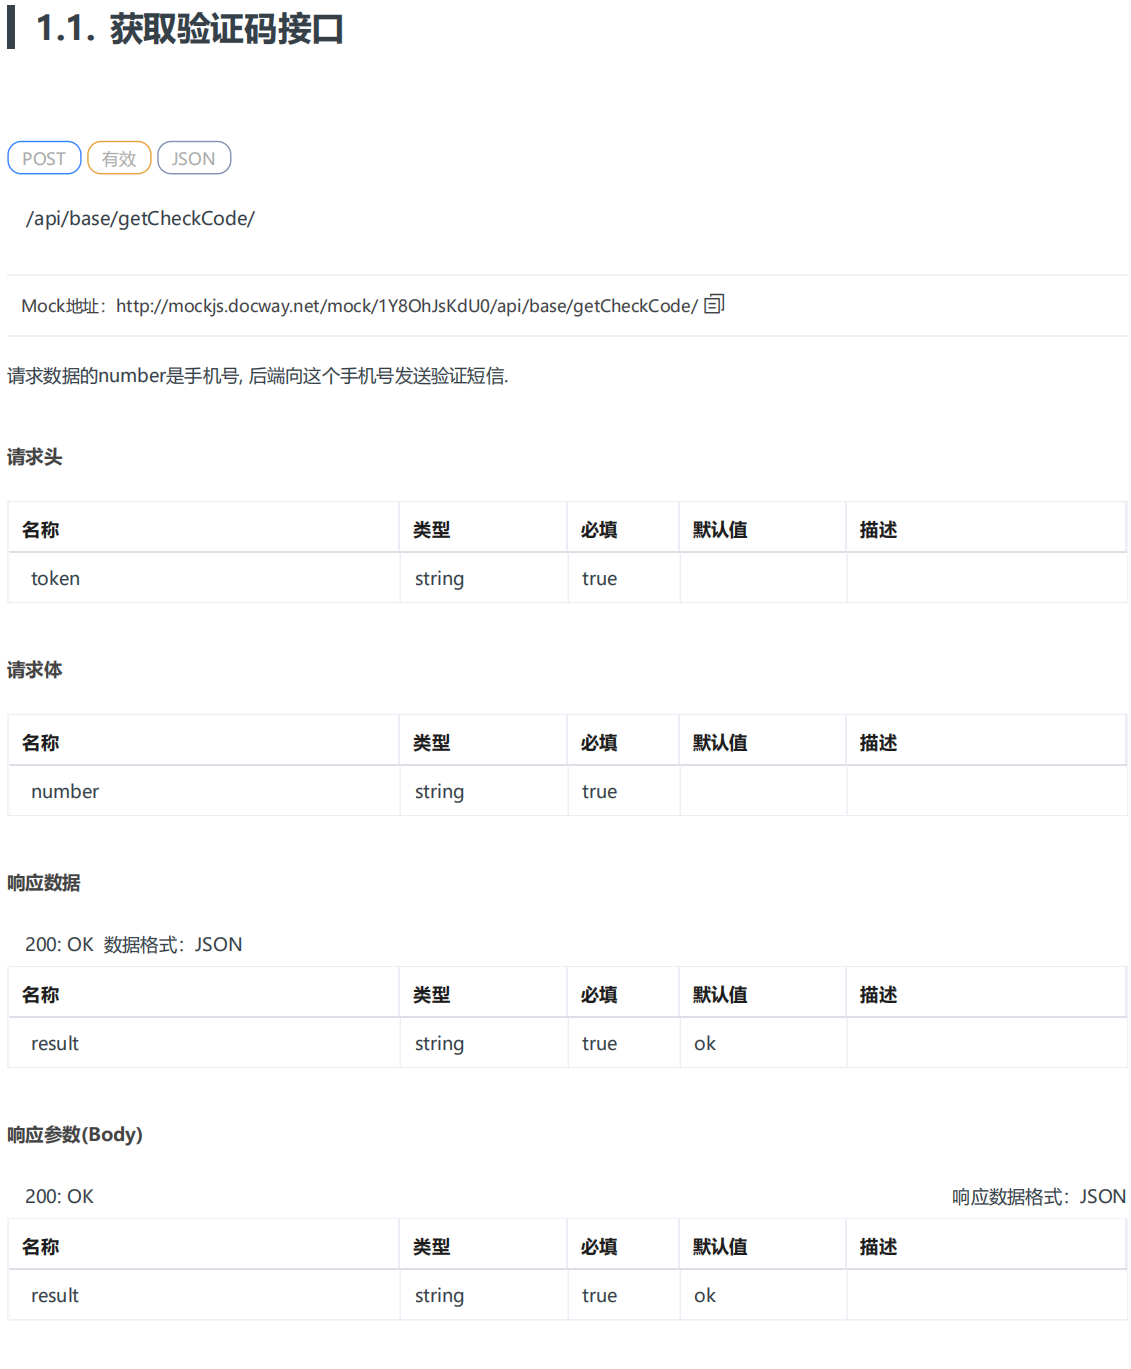
\includegraphics[height=17.0cm,width=14.0cm]{design/image/api1.png} 
    \end{figure}
\newpage
    \subsubsection{登录接口}
    \begin{figure}[h]
        \centering
        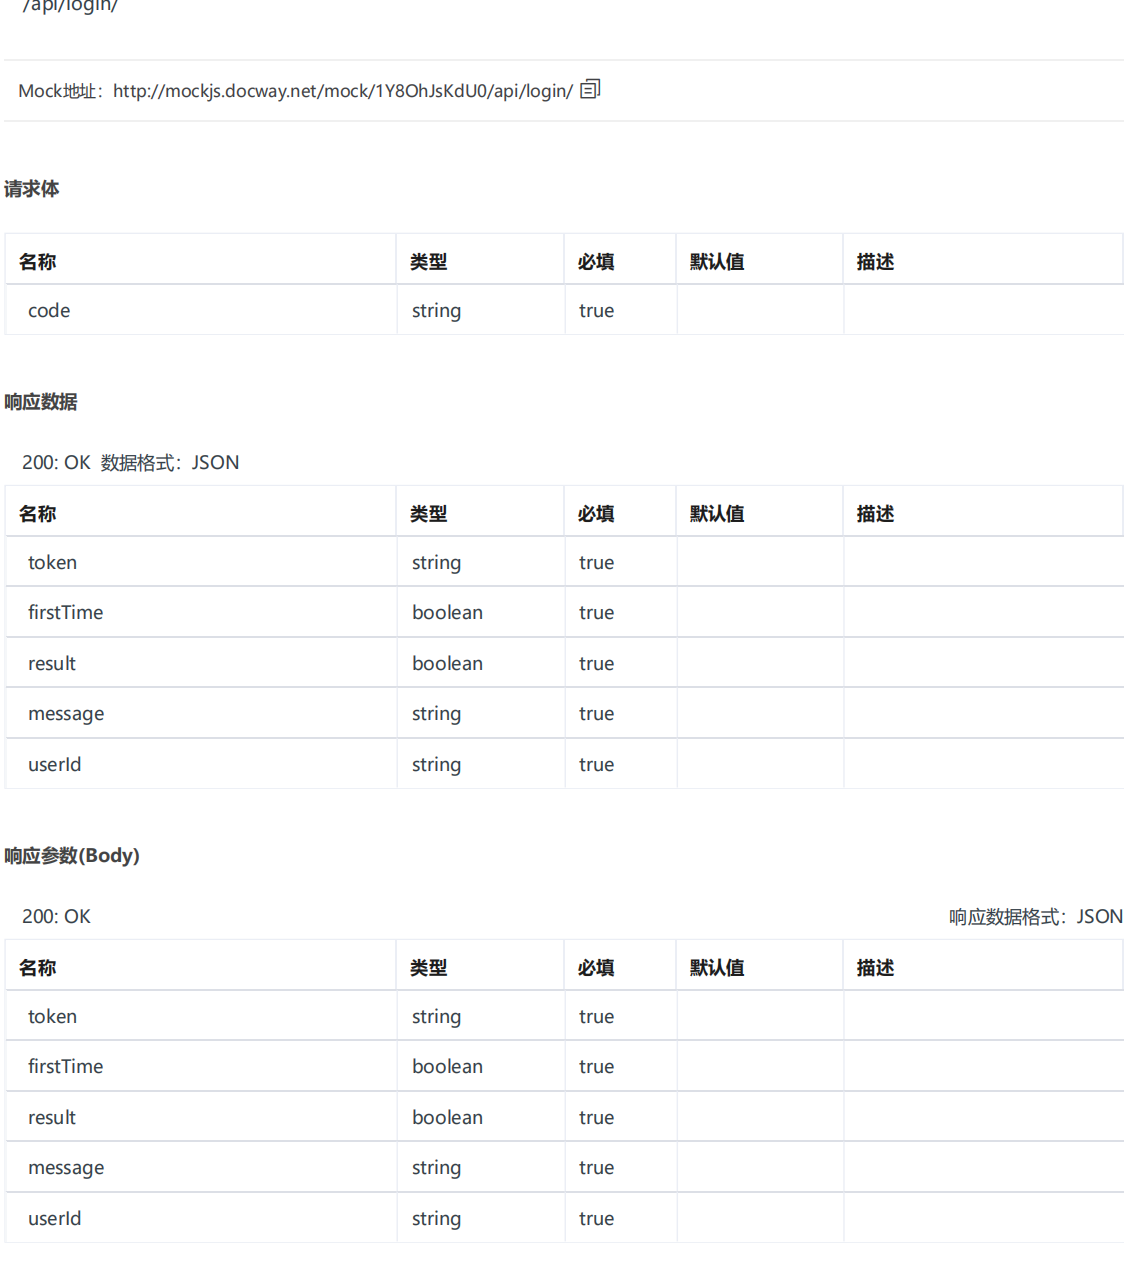
\includegraphics[height=19.0cm,width=14.0cm]{design/image/api2.png} 
        \end{figure}
\newpage        
        \subsubsection{绑定手机号}
        \begin{figure}[h]
            \centering
            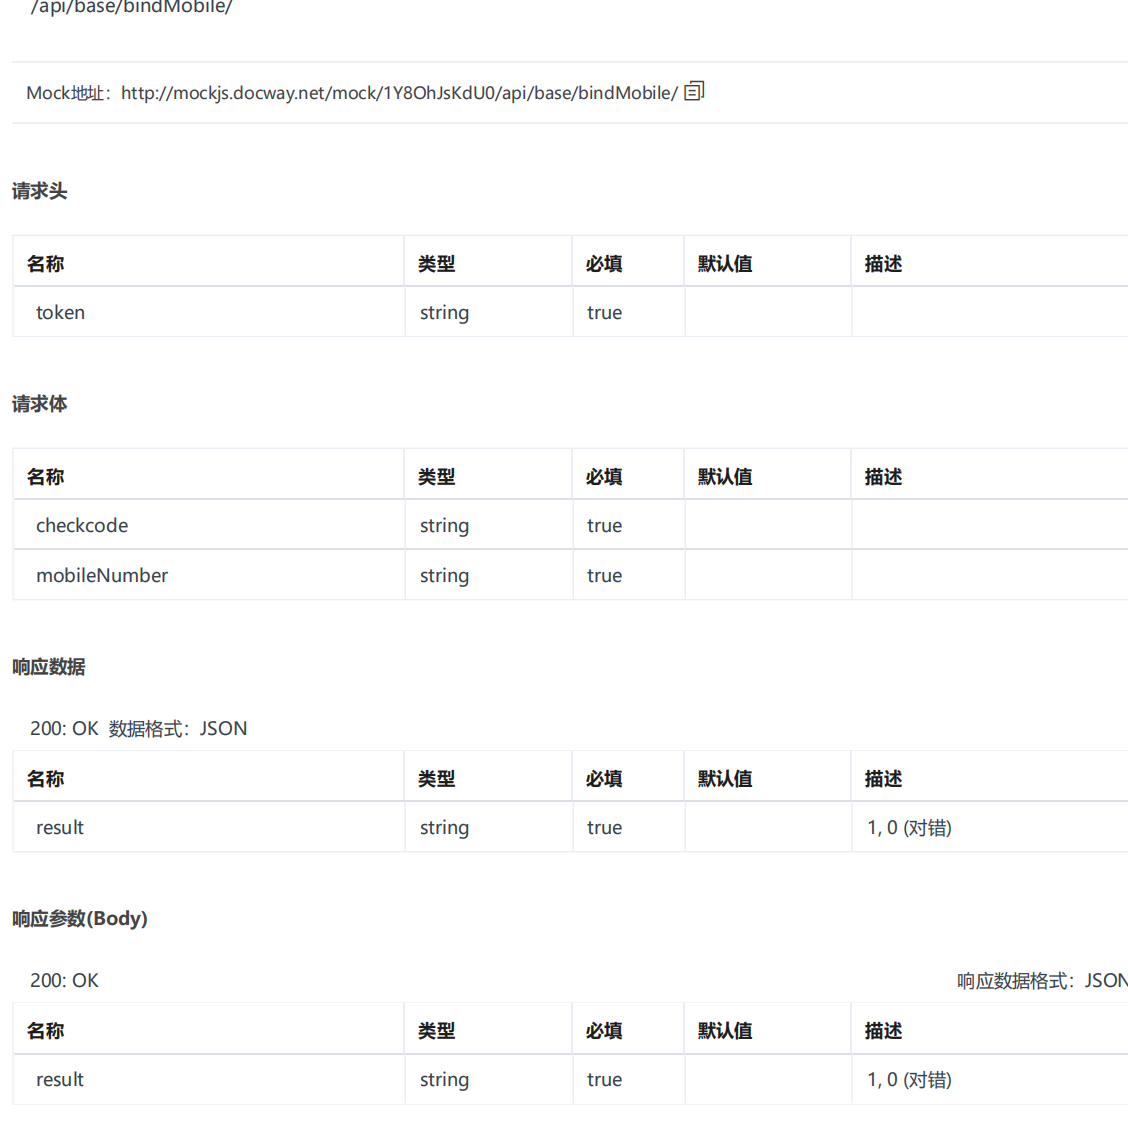
\includegraphics[height=19.0cm,width=14.0cm]{design/image/api3.png} 
            \end{figure}        
            \newpage  
\subsection{主页}
\subsubsection{获取帖子接口}
\begin{figure}[h]
    \centering
    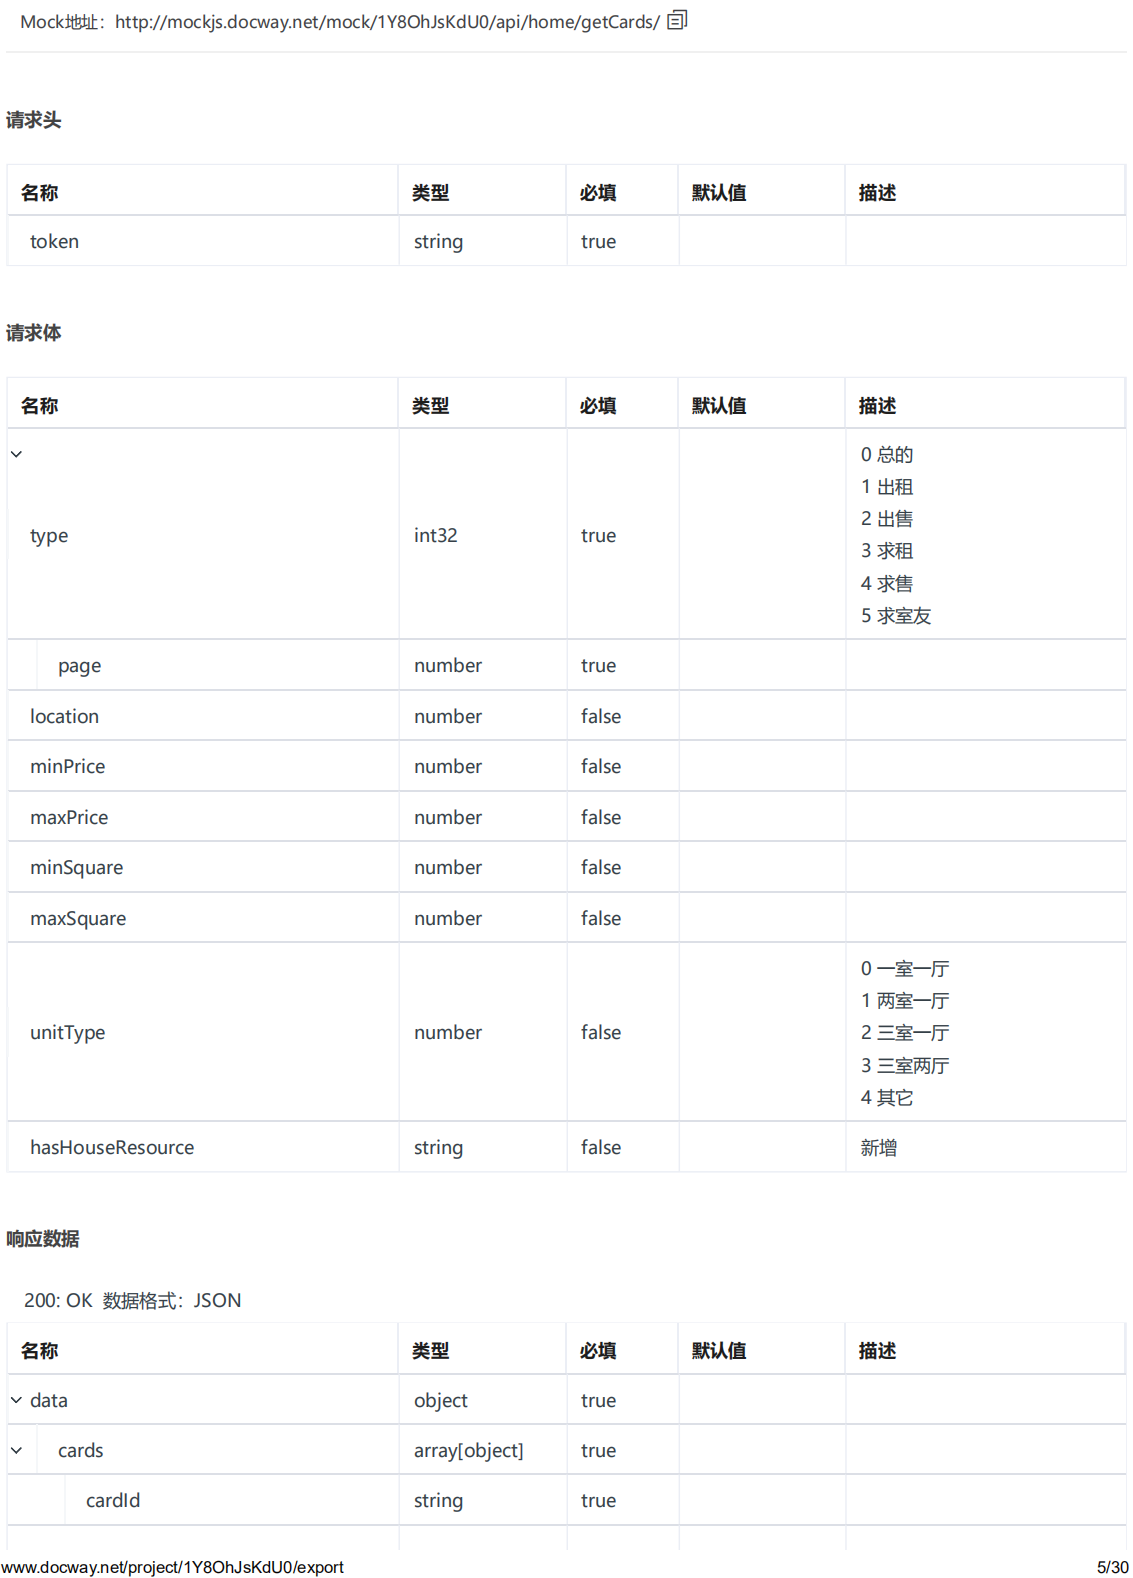
\includegraphics[height=18.0cm,width=14.0cm]{design/image/api4.png} 
    \end{figure}
    \newpage

    \begin{figure}[h]
        \centering
        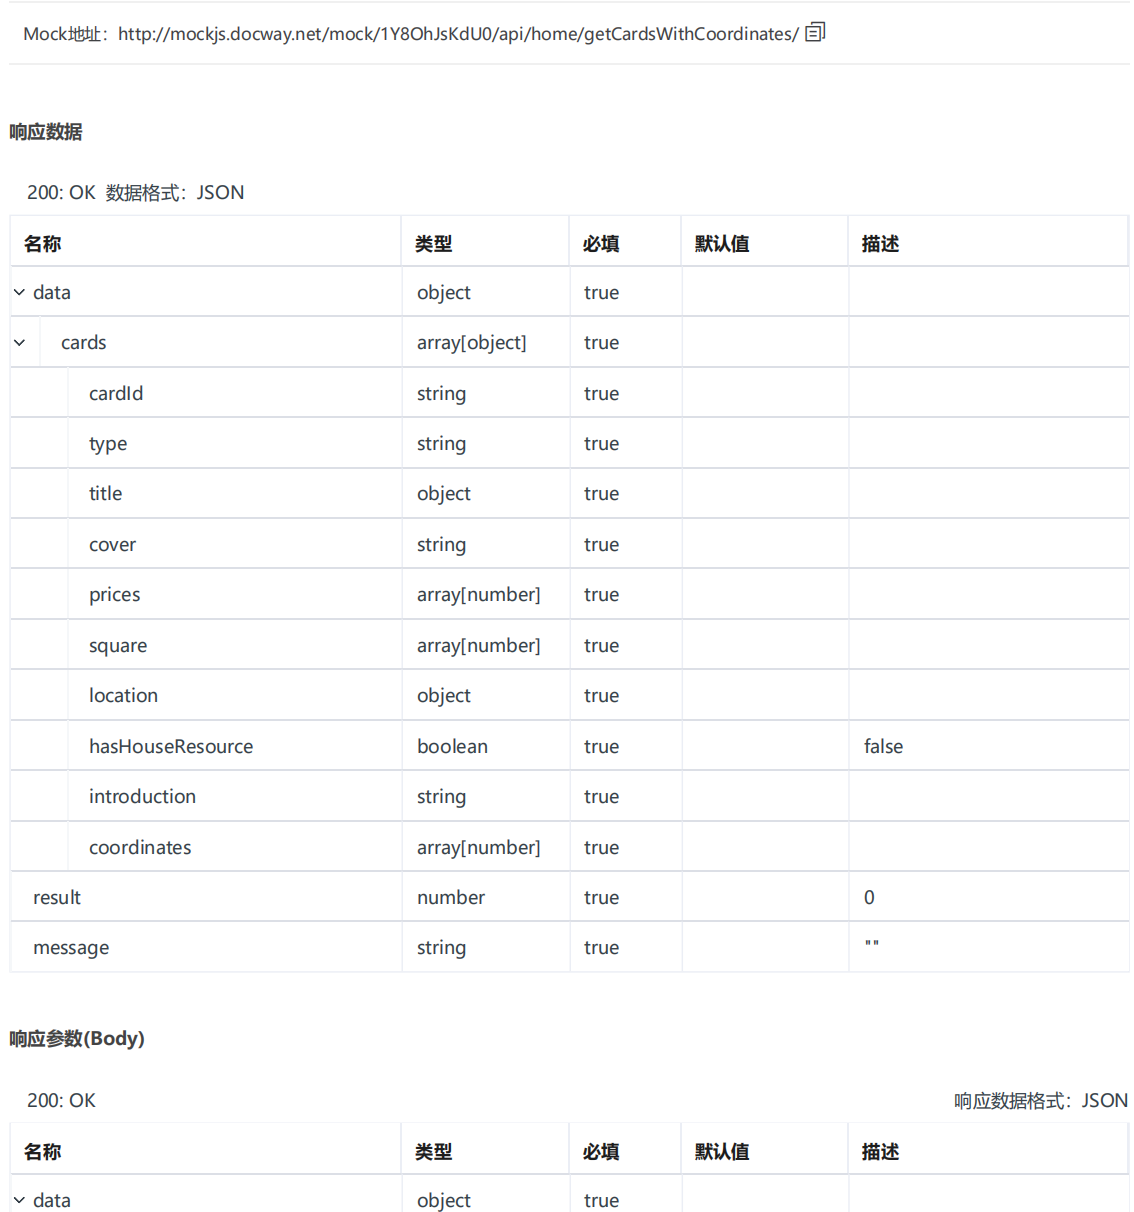
\includegraphics[height=17.0cm,width=14.0cm]{design/image/api5.png} 
        \end{figure}    
    \newpage    
        \subsubsection{获取地图点}        
        \begin{figure}[h]
            \centering
            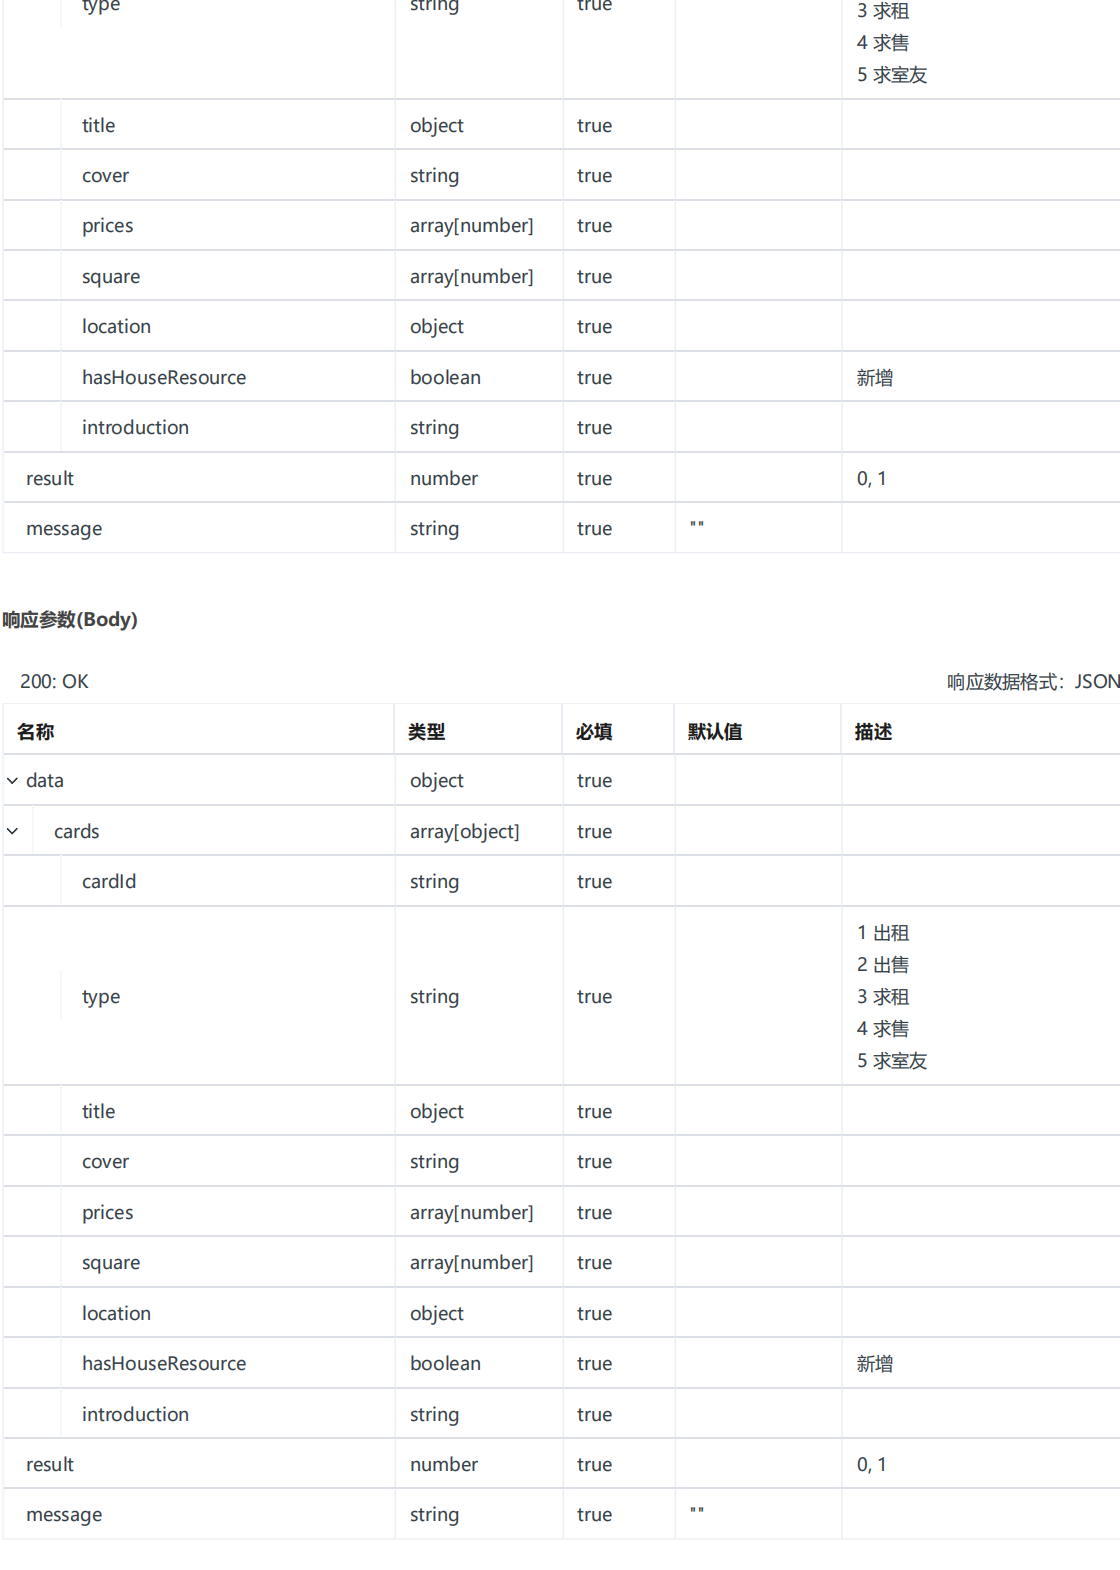
\includegraphics[height=18.0cm,width=14.0cm]{design/image/api6.png} 
            \end{figure}    
    \newpage     
    \begin{figure}[h]
        \centering
        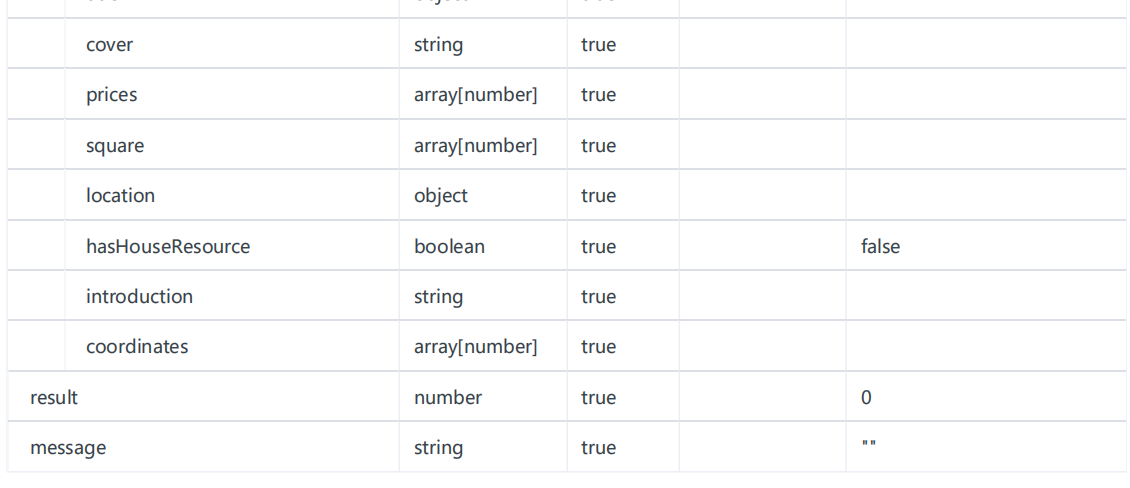
\includegraphics[height=10.0cm,width=14.0cm]{design/image/api7.png} 
        \end{figure}    
\newpage   
    \subsection{详情页}
    \subsubsection{获取详情页数据}
    \begin{figure}[h]
        \centering
        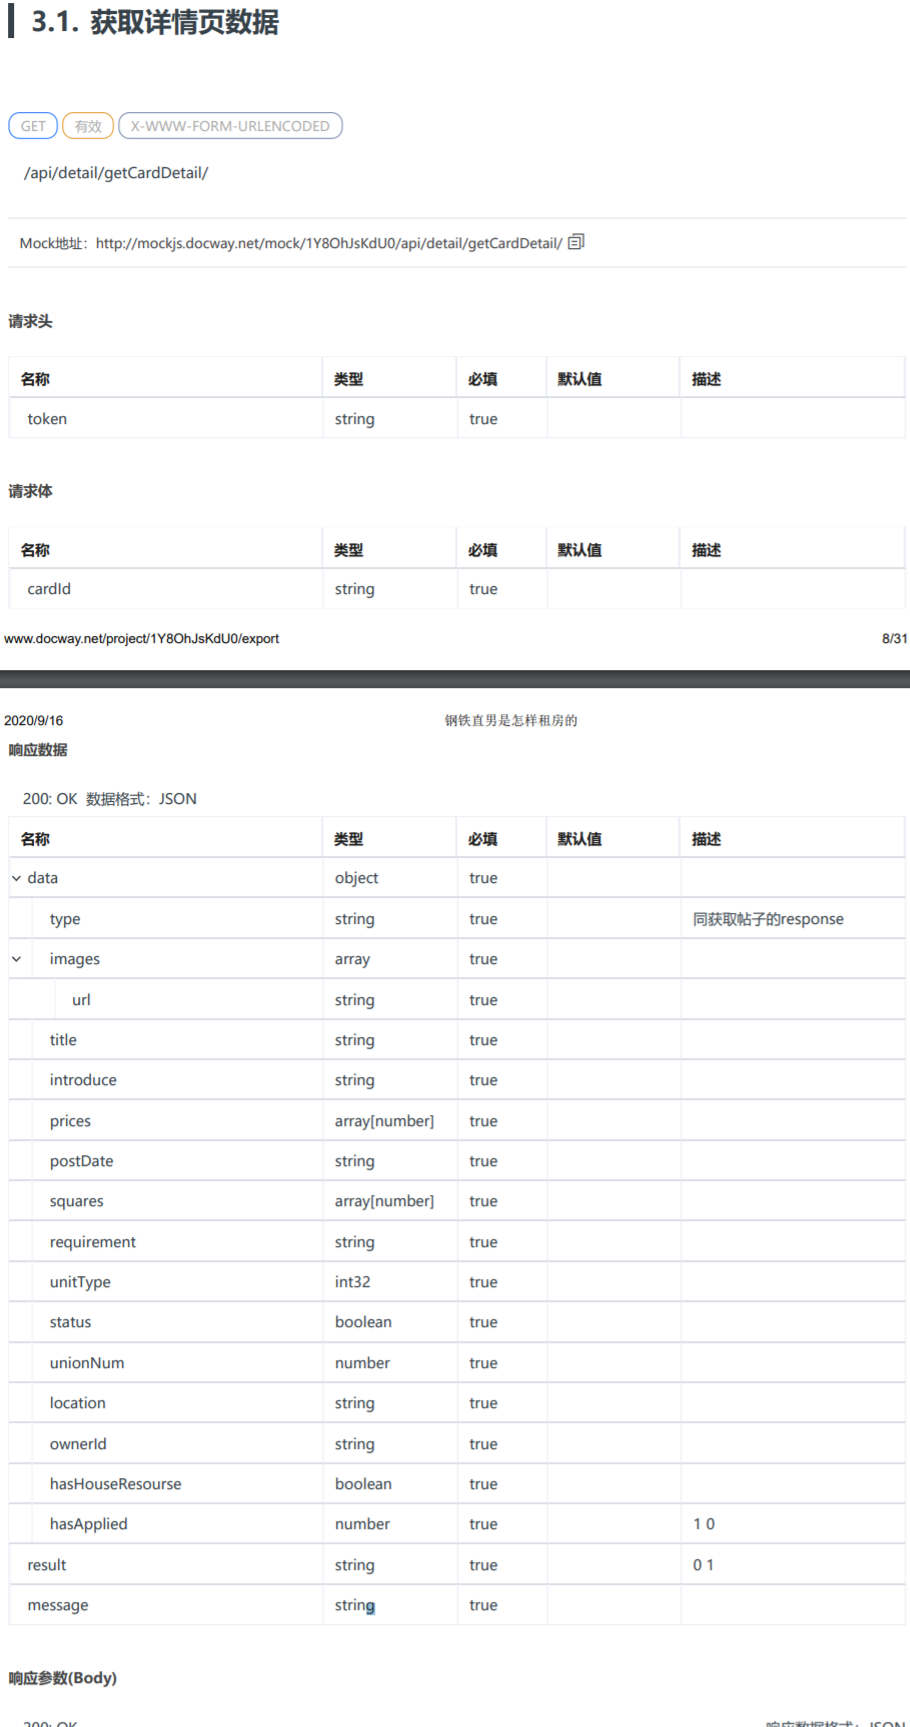
\includegraphics[height=19.0cm,width=14.0cm]{design/image/api8.png} 
        \end{figure}
        \newpage   
        \begin{figure}[h]
            \centering
            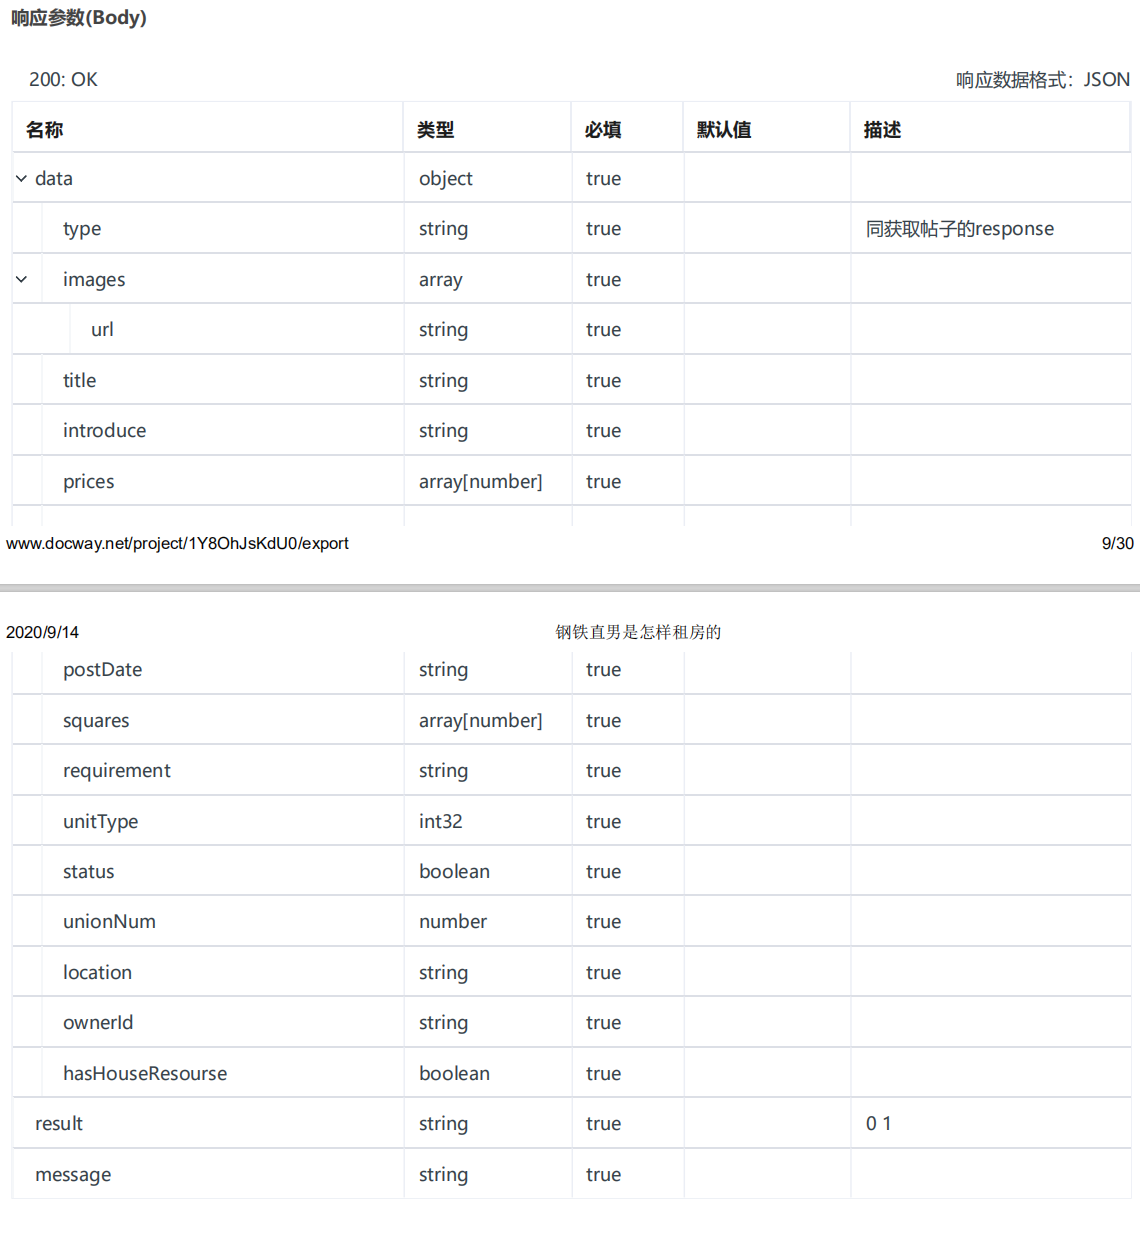
\includegraphics[height=19.0cm,width=14.0cm]{design/image/api9.png} 
            \end{figure}  
            \newpage   
            \subsubsection{个人申请}  
            \begin{figure}[h]
                \centering
                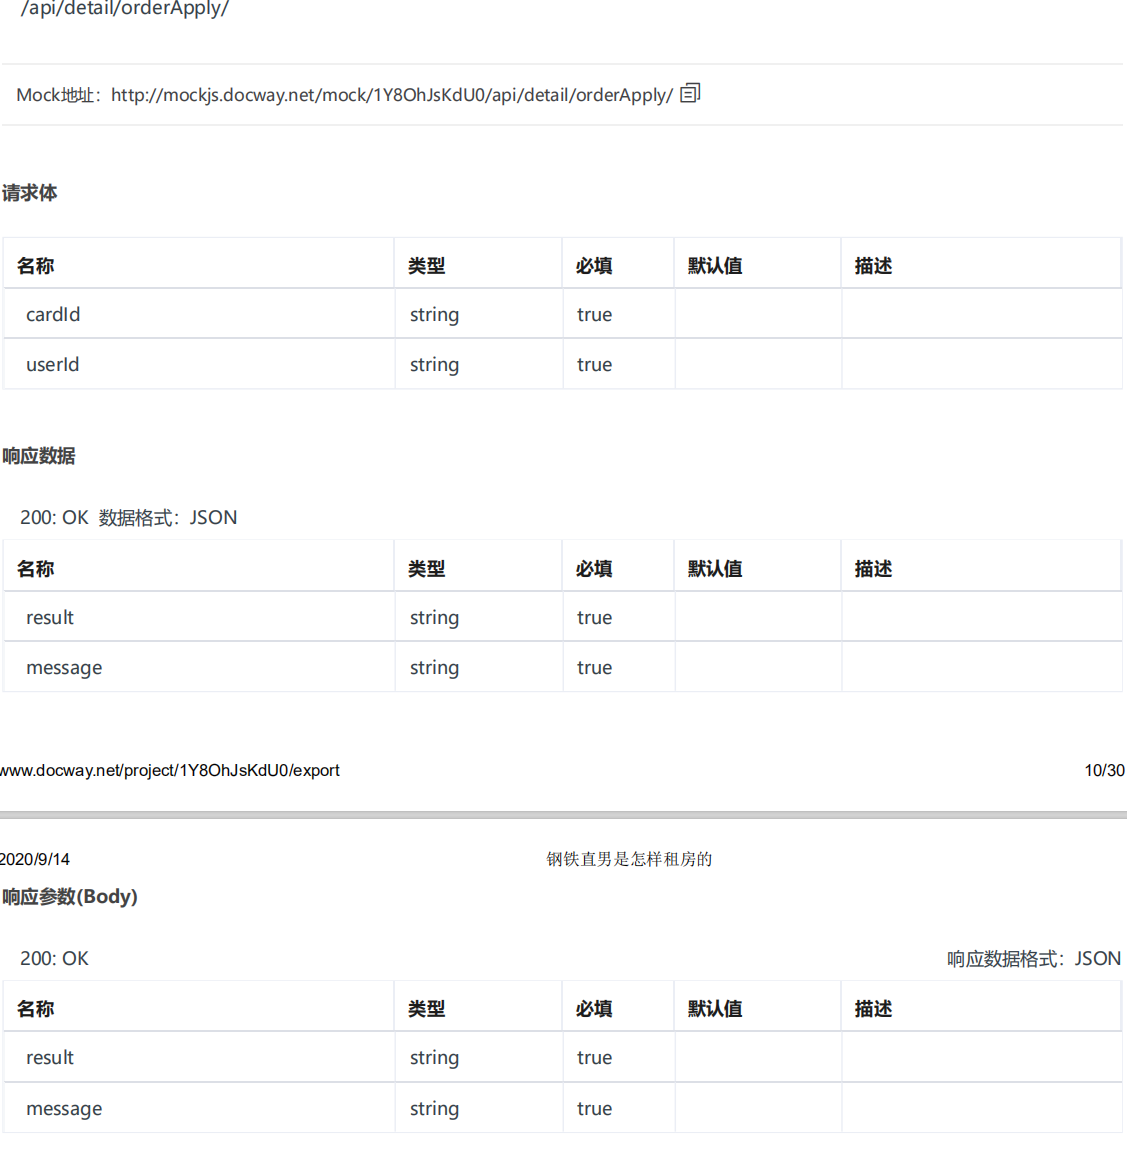
\includegraphics[height=19.0cm,width=14.0cm]{design/image/api10.png} 
                \end{figure}  
                \newpage  
                
                \subsubsection{合租申请} 
                \begin{figure}[h]
                    \centering
                    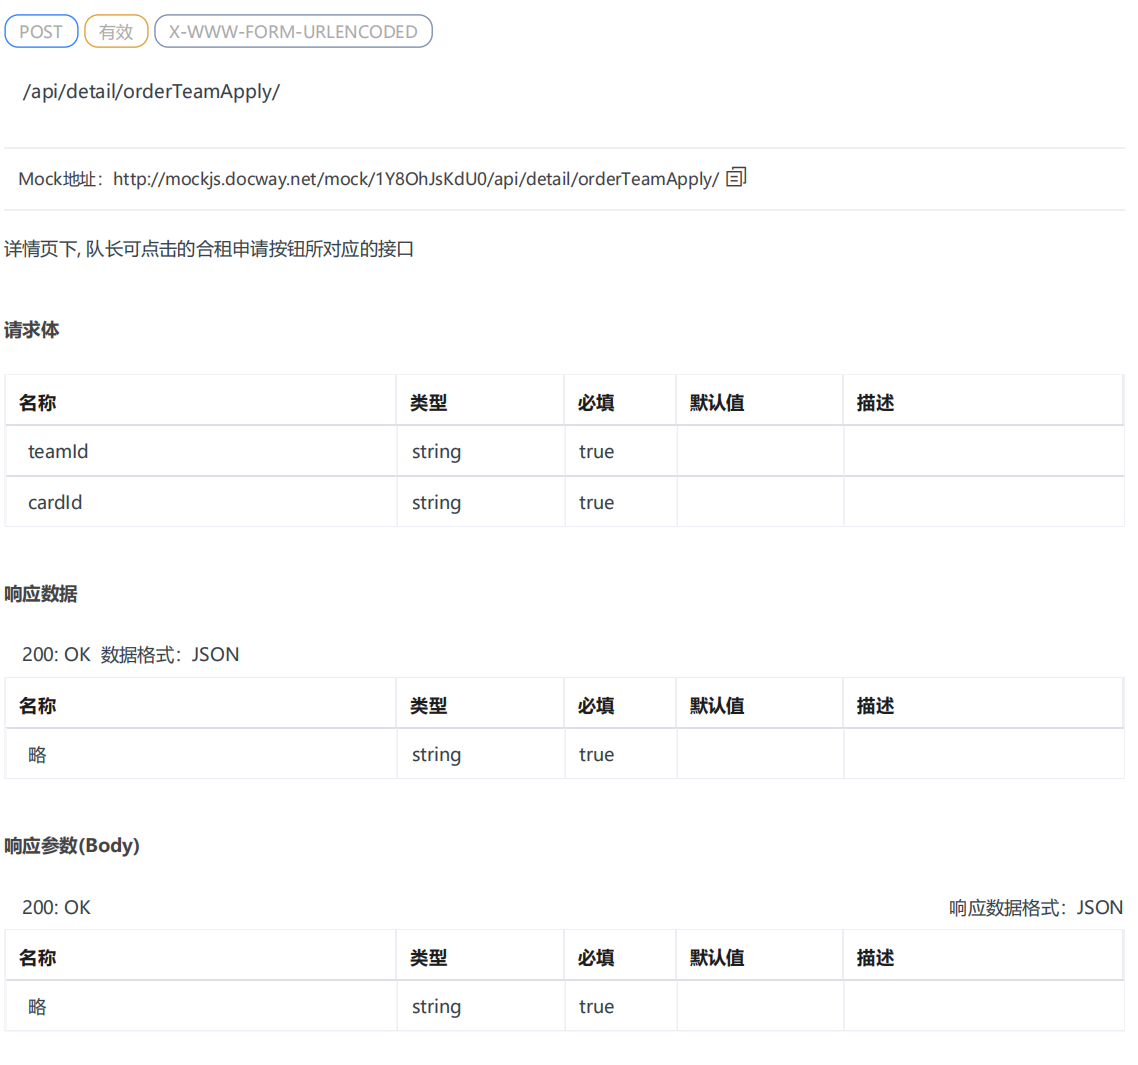
\includegraphics[height=16.0cm,width=14.0cm]{design/image/api11.png} 
                    \end{figure}  
                    \newpage 
                    \subsubsection{房主查阅已申请的个人和队伍} 
                    \begin{figure}[h]
                        \centering
                        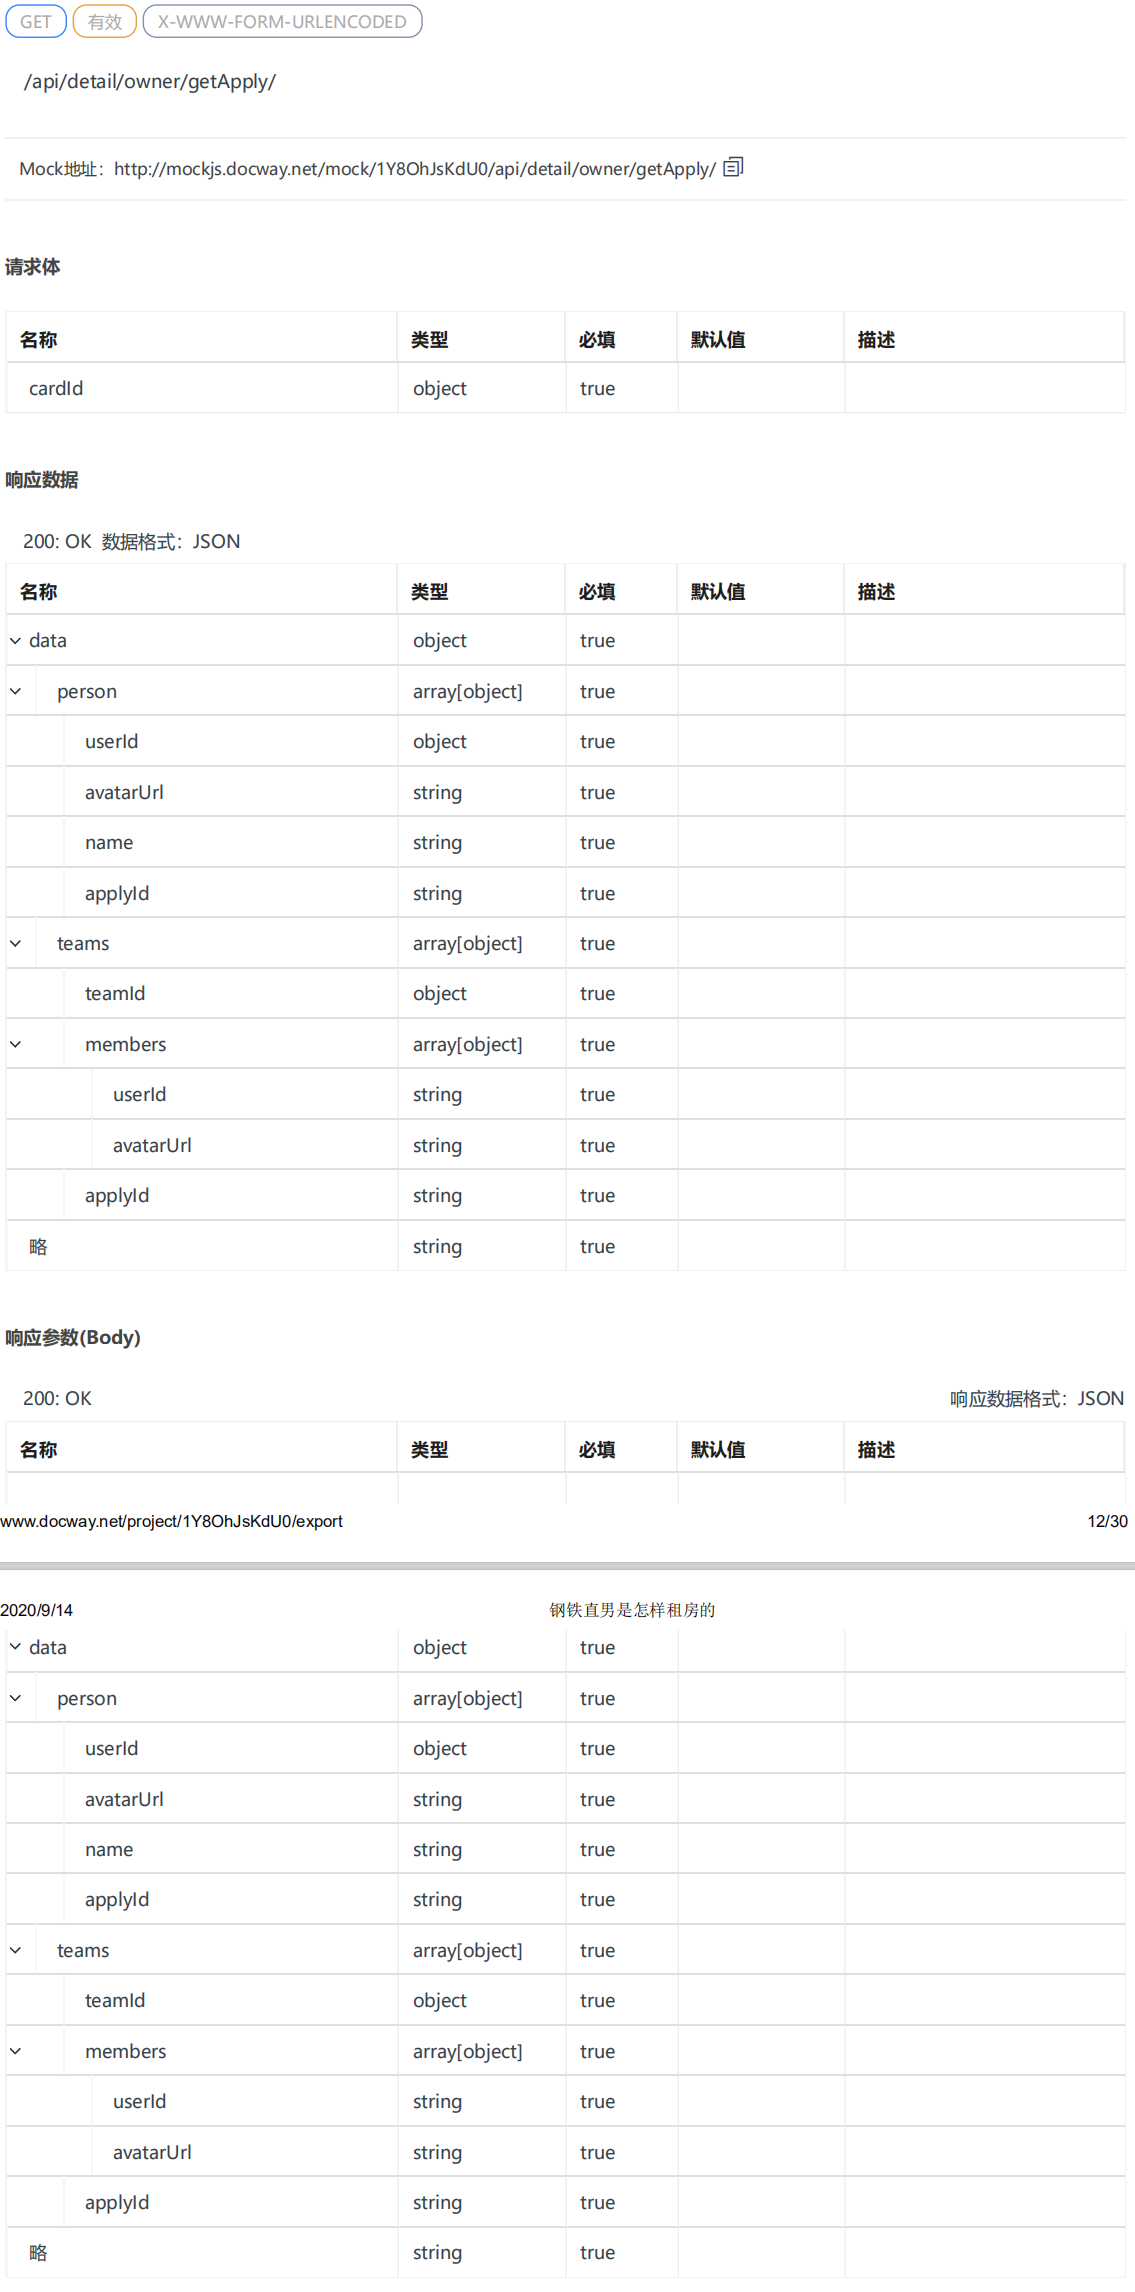
\includegraphics[height=19.0cm,width=14.0cm]{design/image/api12.png} 
                        \end{figure}  
                        \newpage   
                        \subsubsection{房主查阅已申请的个人和队伍} 
                        \begin{figure}[h]
                            \centering
                            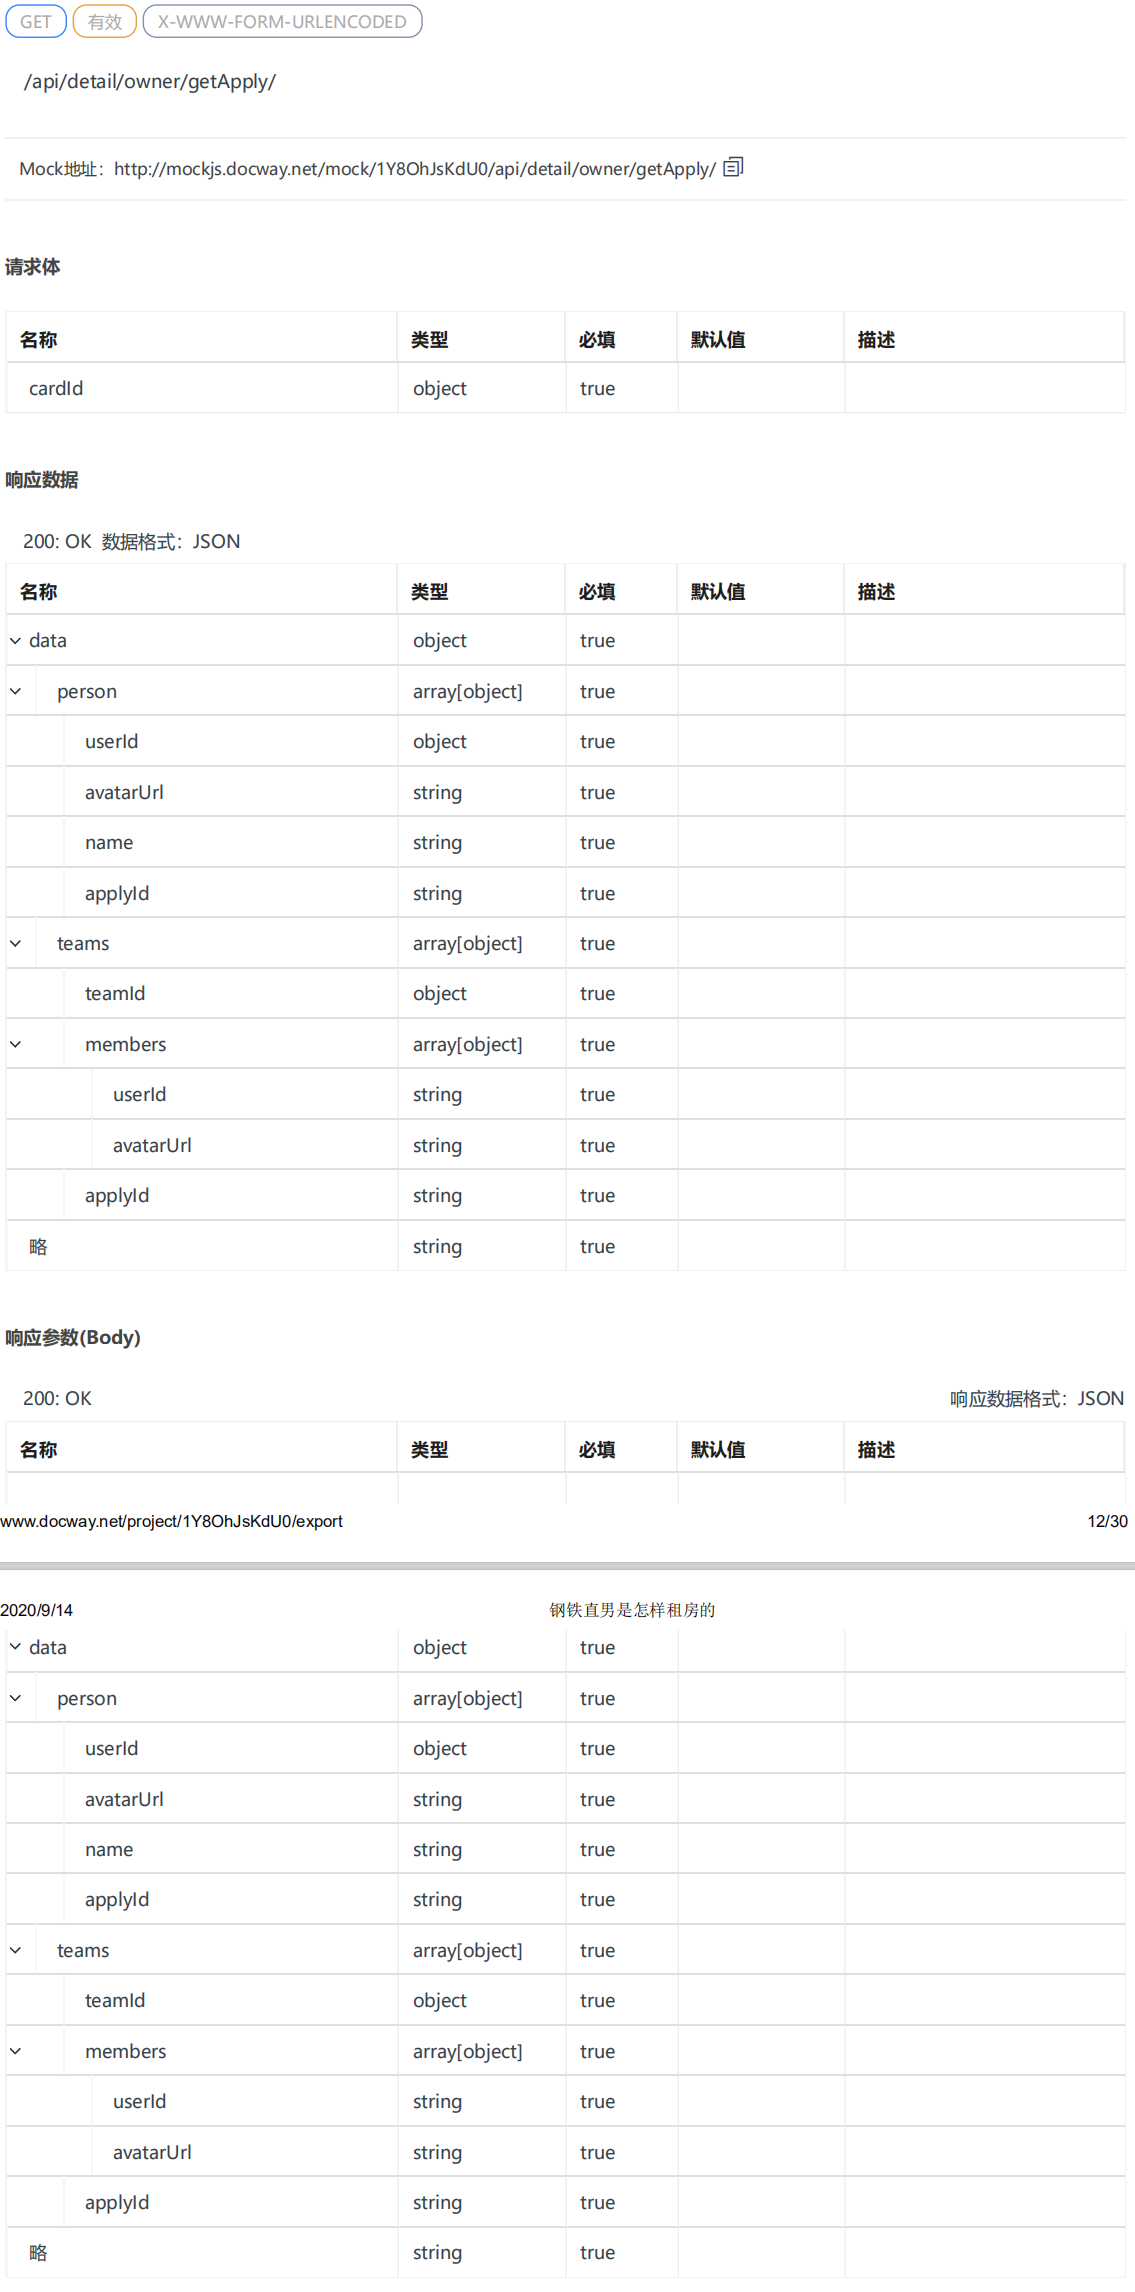
\includegraphics[height=19.0cm,width=14.0cm]{design/image/api12.png} 
                            \end{figure}  
                            \newpage    
                            \subsubsection{房主查阅已申请的个人和队伍} 
                            \begin{figure}[h]
                                \centering
                                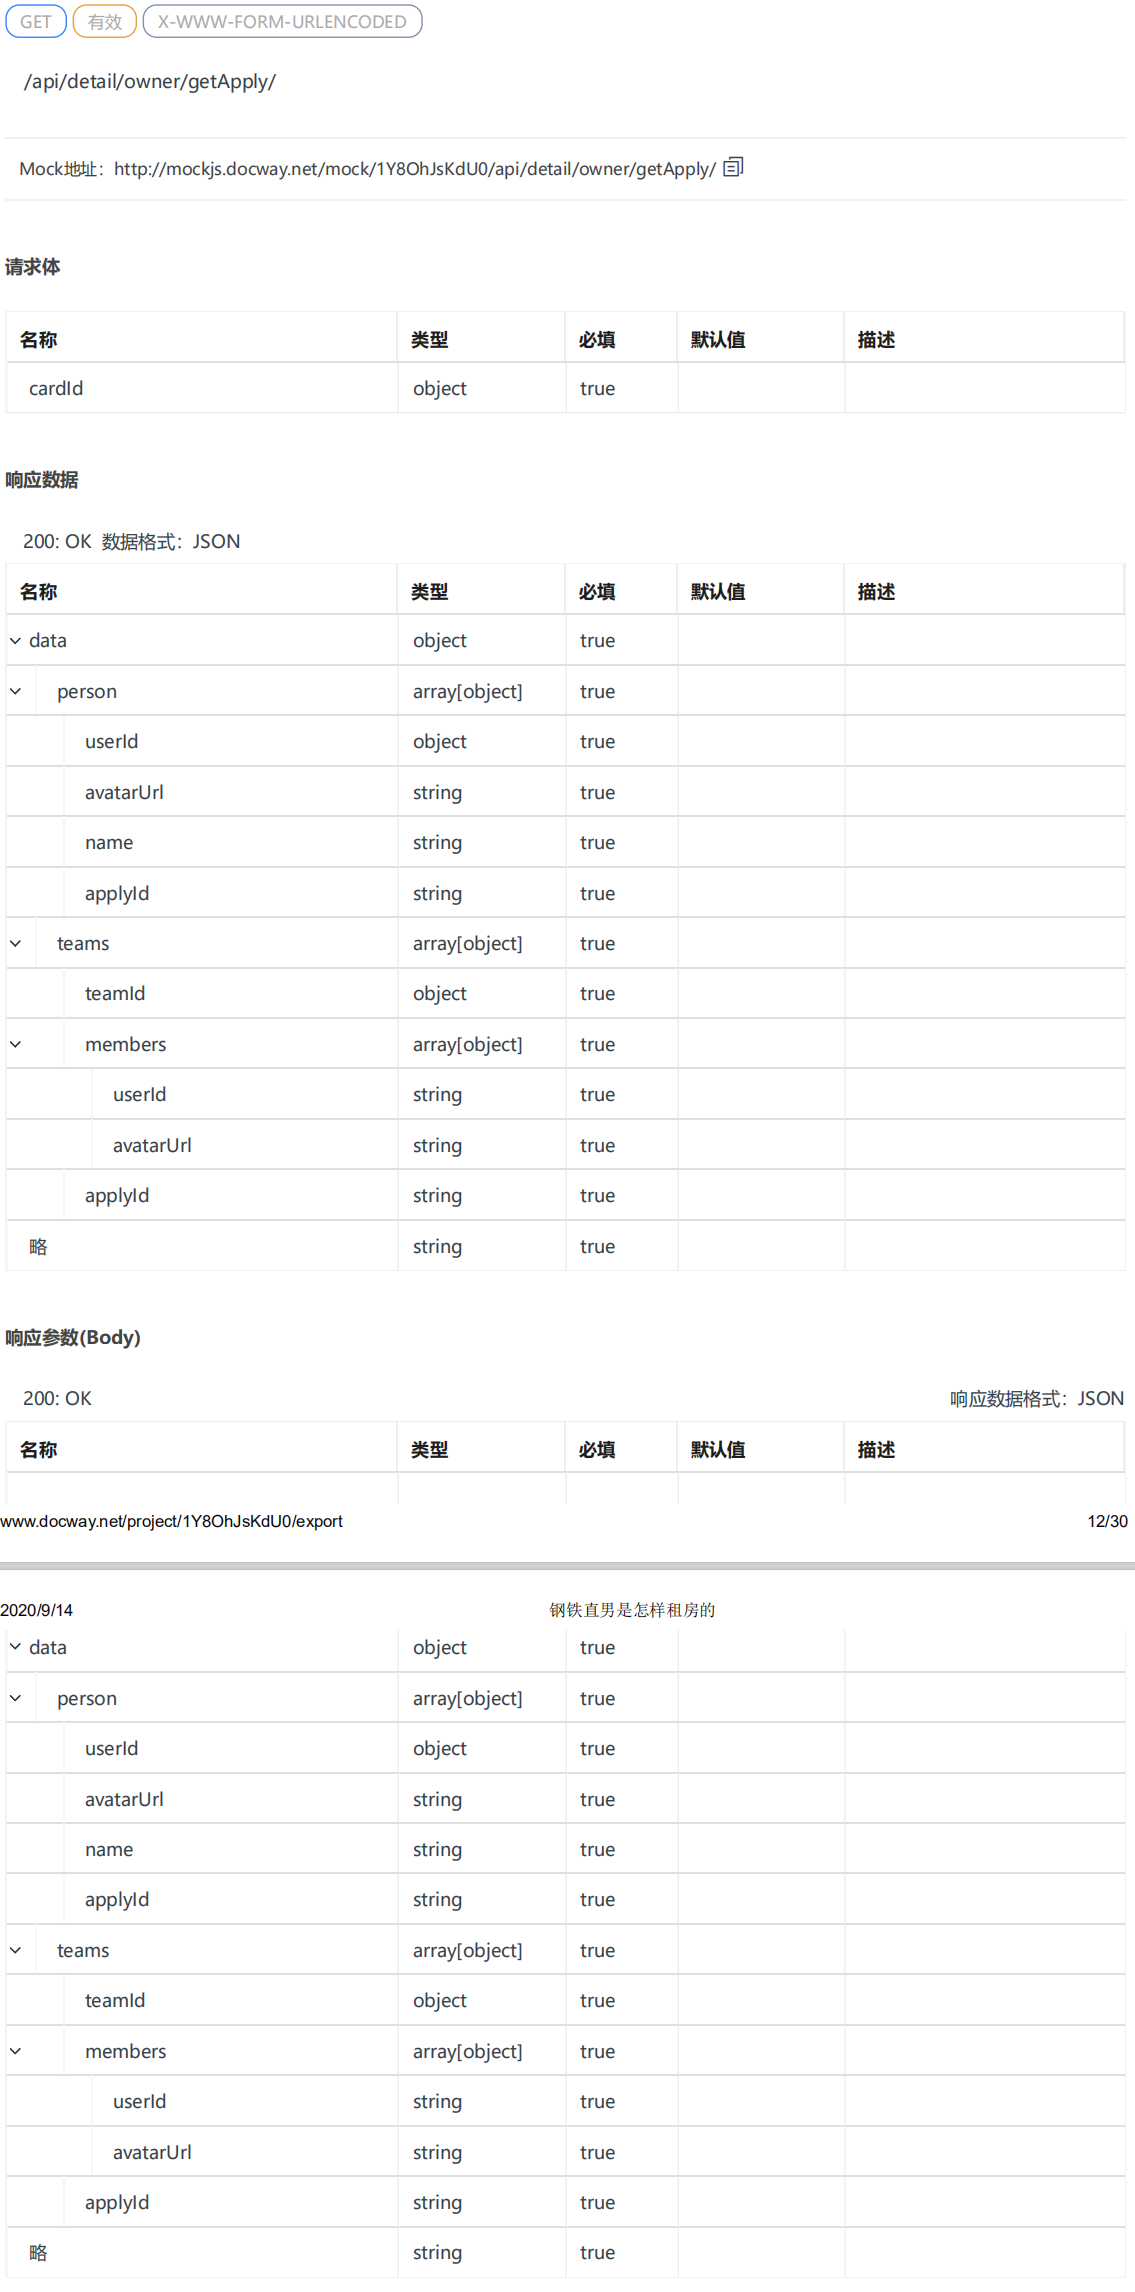
\includegraphics[height=19.0cm,width=14.0cm]{design/image/api12.png} 
                                \end{figure}  
                                \newpage                         \subsubsection{处理申请} 
                        \begin{figure}[h]
                            \centering
                            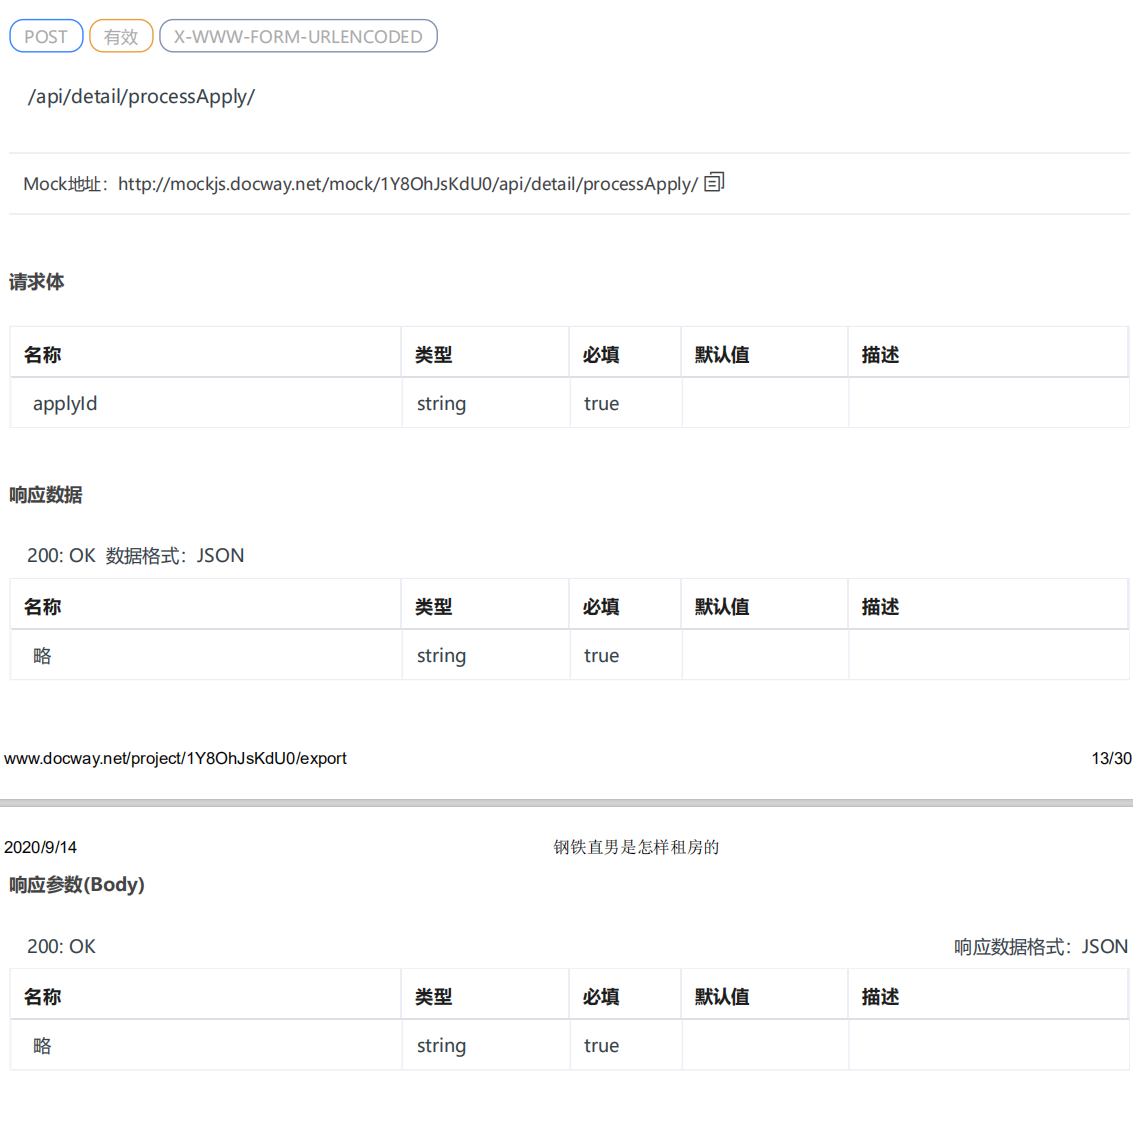
\includegraphics[height=19.0cm,width=14.0cm]{design/image/api13.png} 
                            \end{figure}  
                            \newpage  
        \subsection{合租}
        \subsubsection{获取合租队列} 
                        \begin{figure}[h]
                            \centering
                            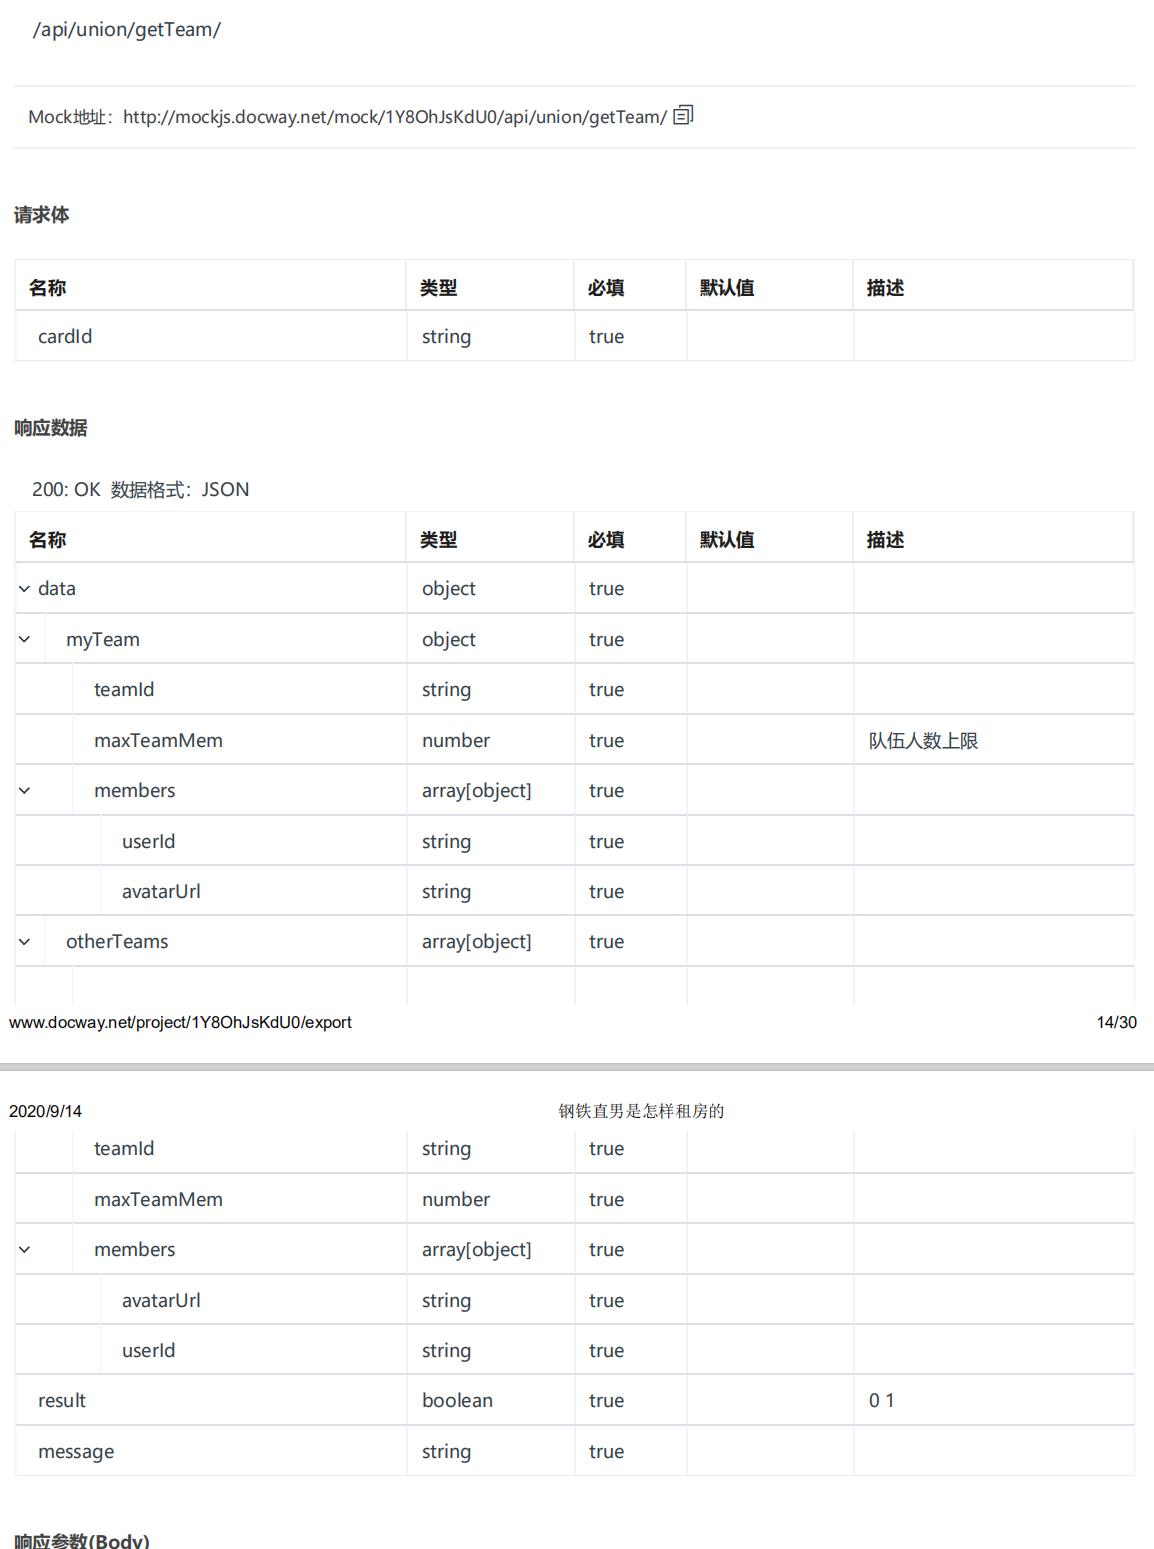
\includegraphics[height=19.0cm,width=14.0cm]{design/image/api14.png} 
                            \end{figure}  
                            \newpage                
 
                            \begin{figure}[h]
                                \centering
                                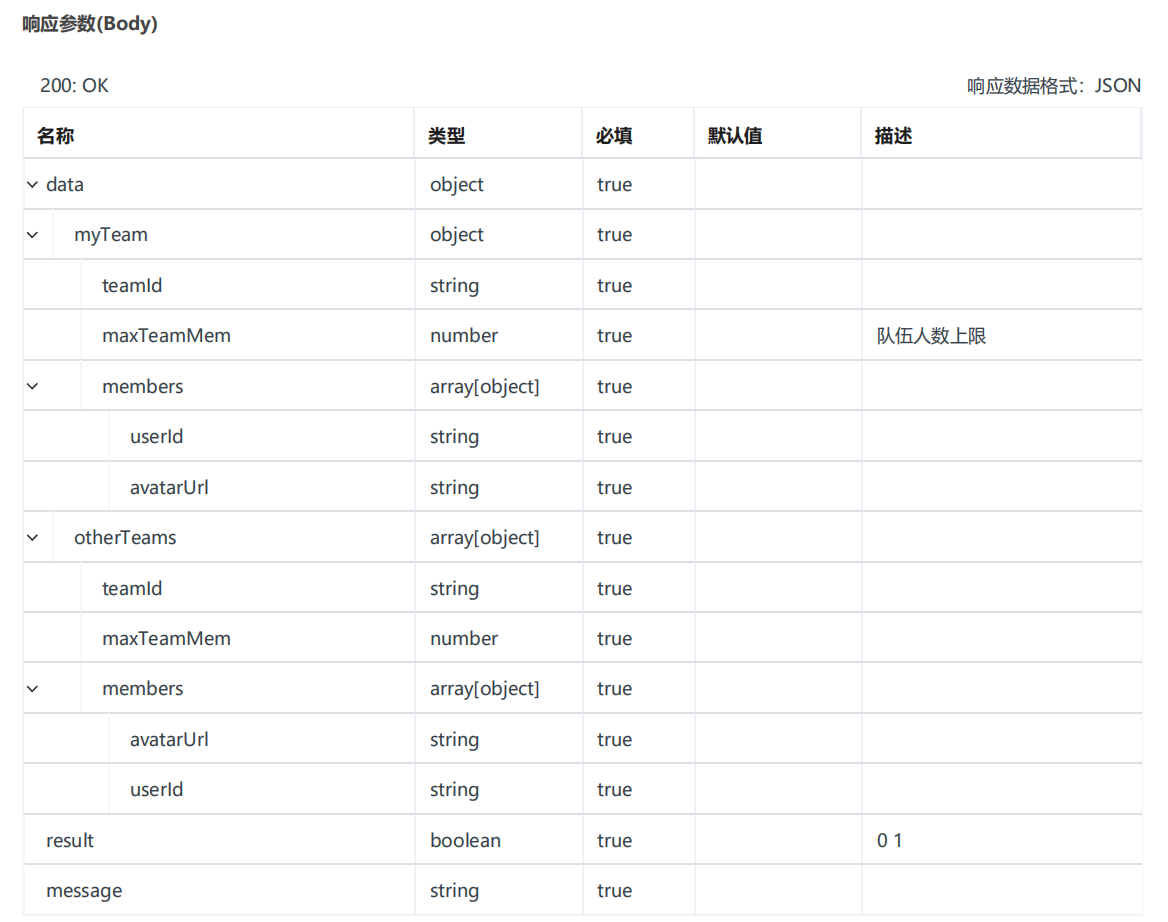
\includegraphics[height=16.0cm,width=14.0cm]{design/image/api15.png} 
                                \end{figure}  
                                \newpage              
        \subsubsection{新建合租队伍}
        \begin{figure}[h]
            \centering
            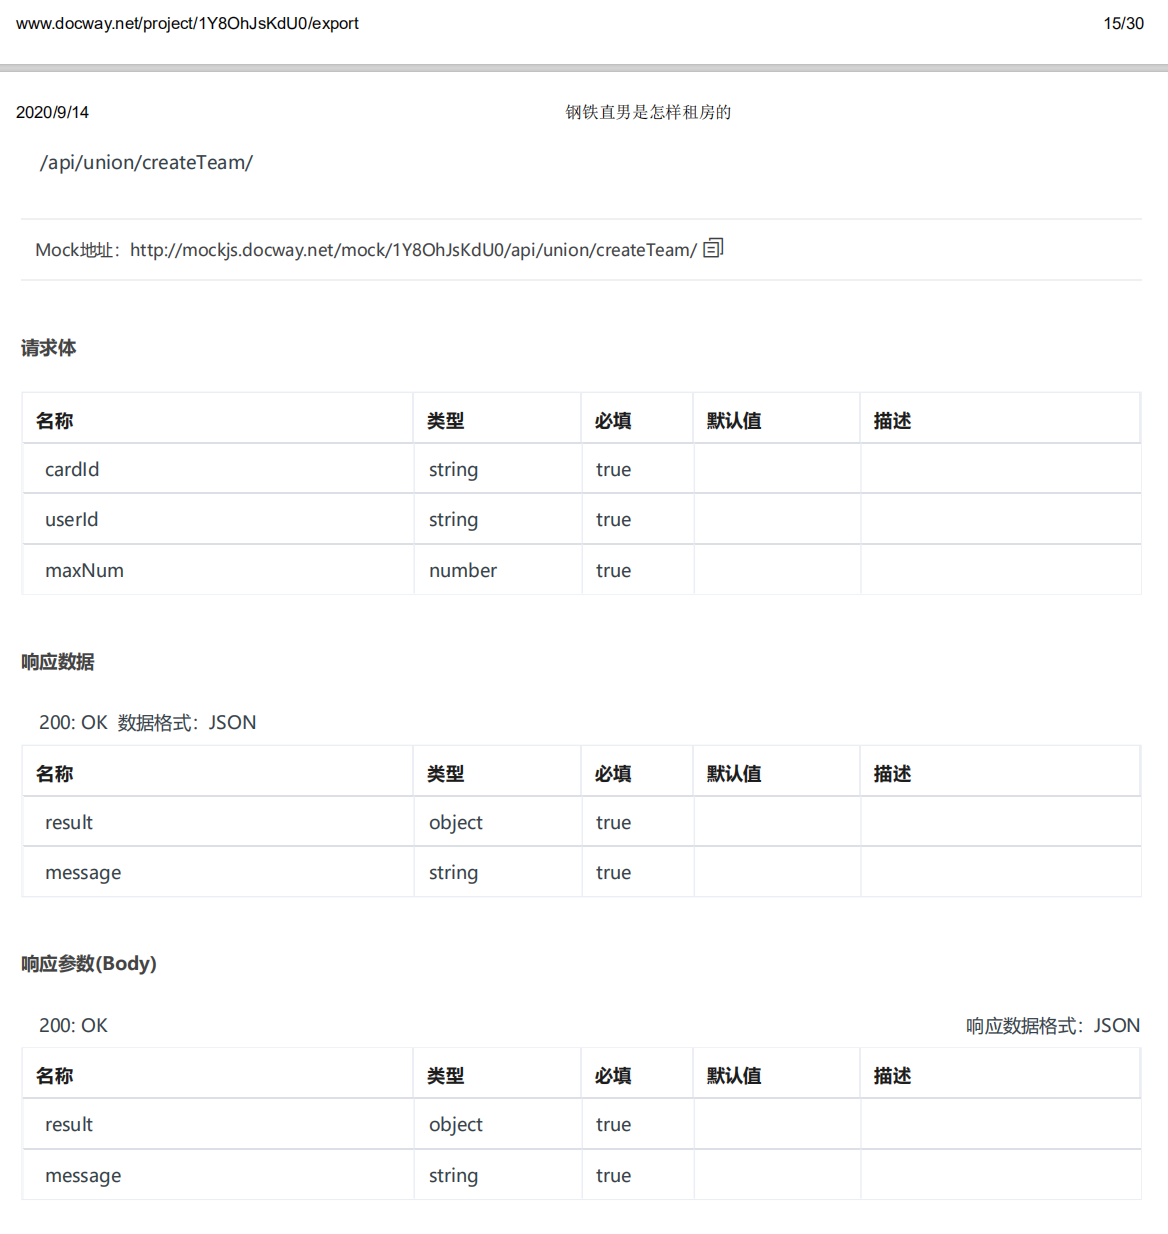
\includegraphics[height=19.0cm,width=14.0cm]{design/image/api16.png} 
            \end{figure}  
            \newpage                                  
        \subsubsection{加入合租队伍}
        \begin{figure}[h]
            \centering
            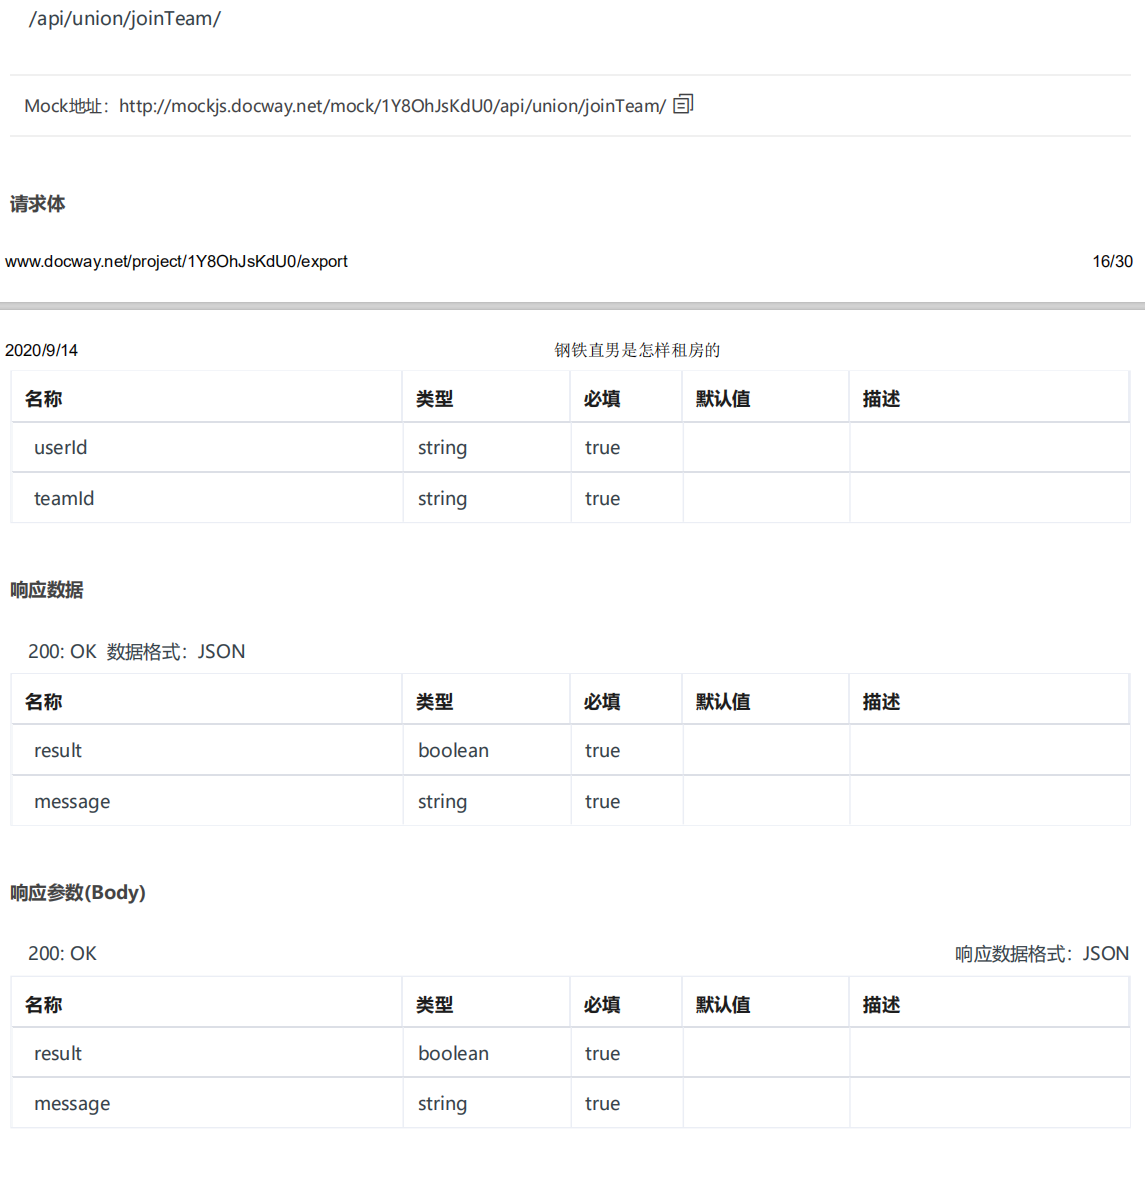
\includegraphics[height=19.0cm,width=14.0cm]{design/image/api17.png} 
            \end{figure}  
            \newpage    
            \subsubsection{删除(退出)队伍}
            \begin{figure}[h]
                \centering
                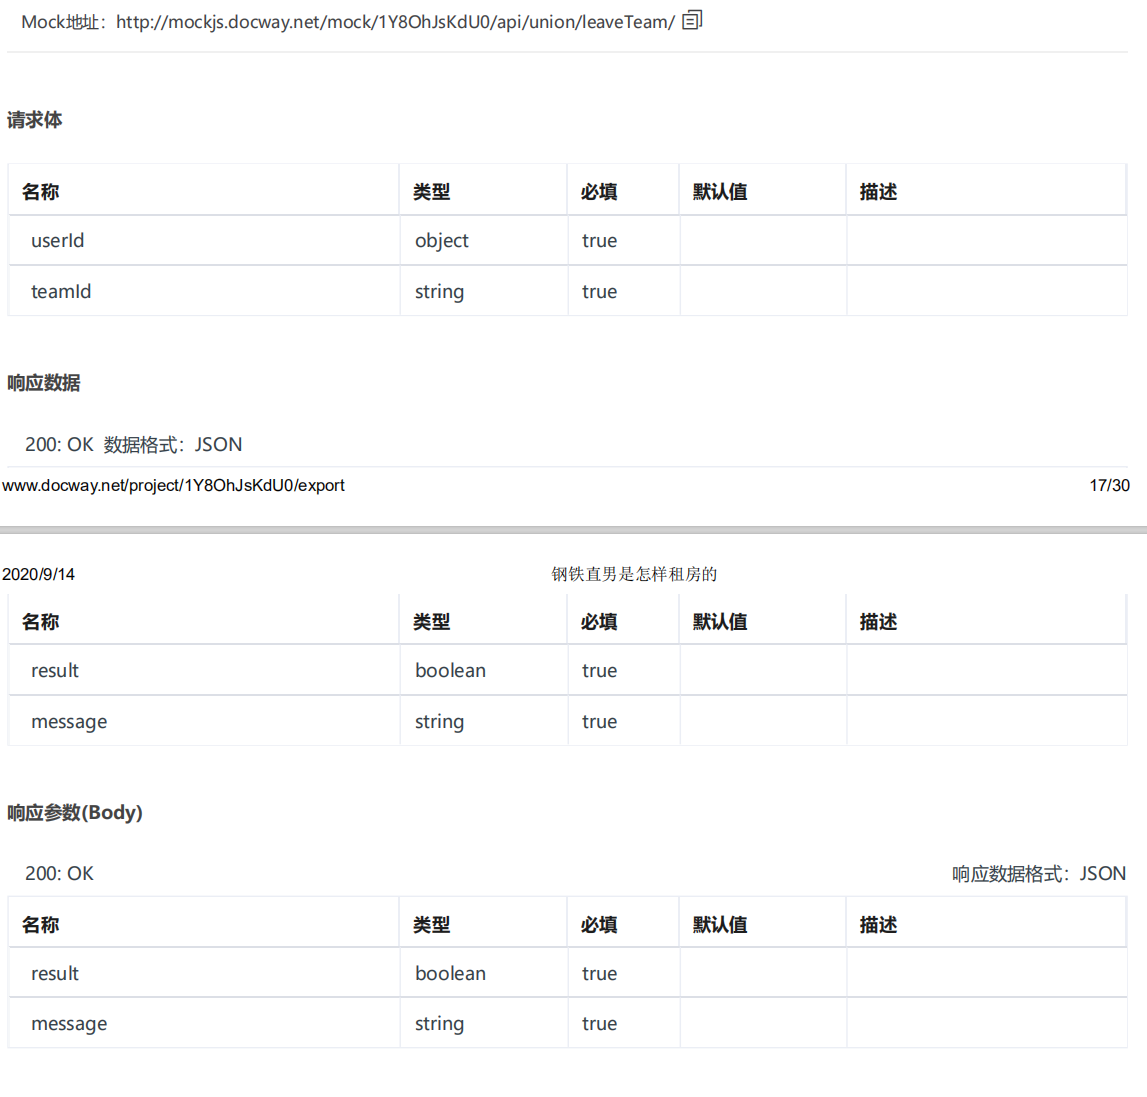
\includegraphics[height=19.0cm,width=14.0cm]{design/image/api18.png} 
                \end{figure}  
                \newpage    
                
        \subsection{评论}  
        \subsubsection{获取评论接口}
        \begin{figure}[h]
            \centering
            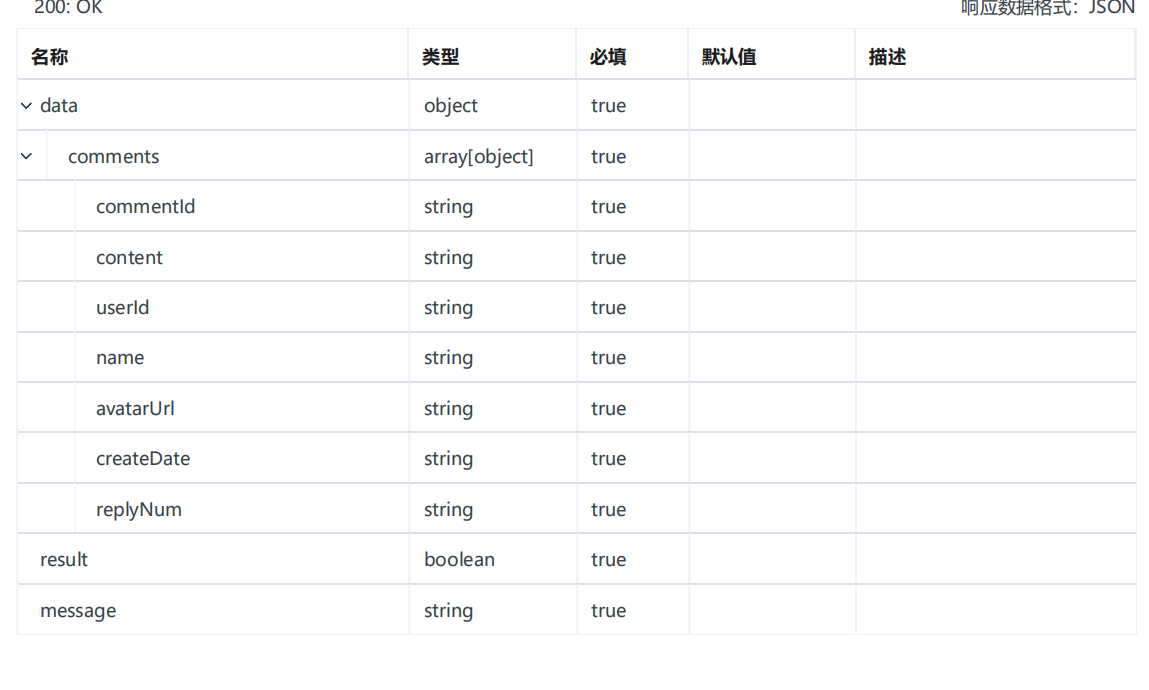
\includegraphics[height=16.0cm,width=14.0cm]{design/image/api20.png} 
            \end{figure}  
            \newpage    
        \subsubsection{获取回复}
        \begin{figure}[h]
            \centering
            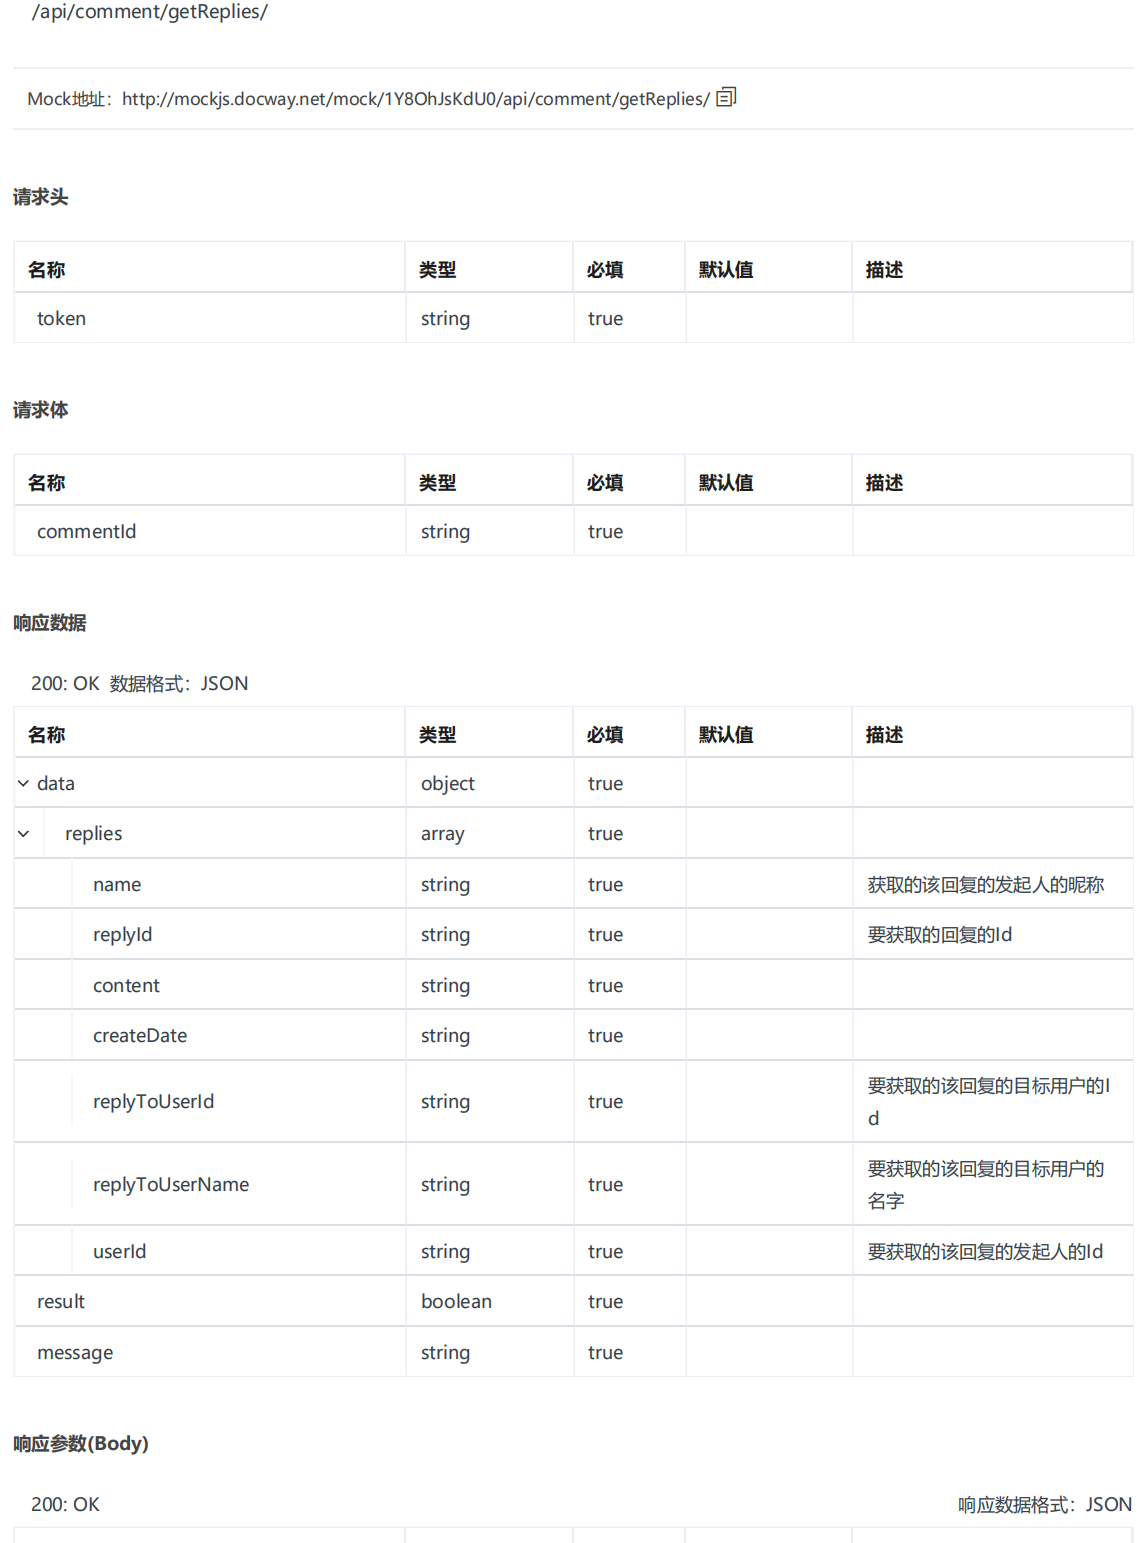
\includegraphics[height=19.0cm,width=14.0cm]{design/image/api21.png} 
            \end{figure}  
            \newpage    
            \begin{figure}[h]
                \centering
                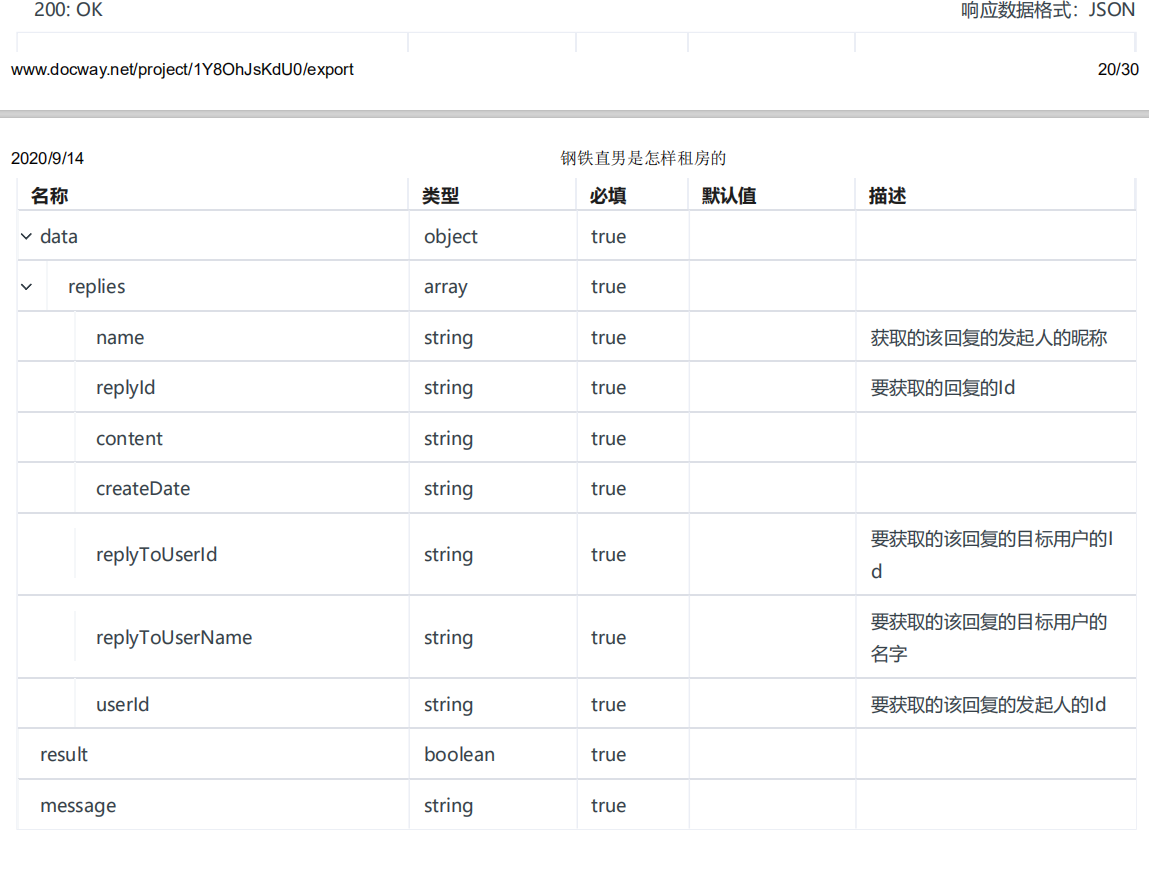
\includegraphics[height=14.0cm,width=14.0cm]{design/image/api22.png} 
                \end{figure}  
                \newpage    
        \subsubsection{提交评论}
        \begin{figure}[h]
            \centering
            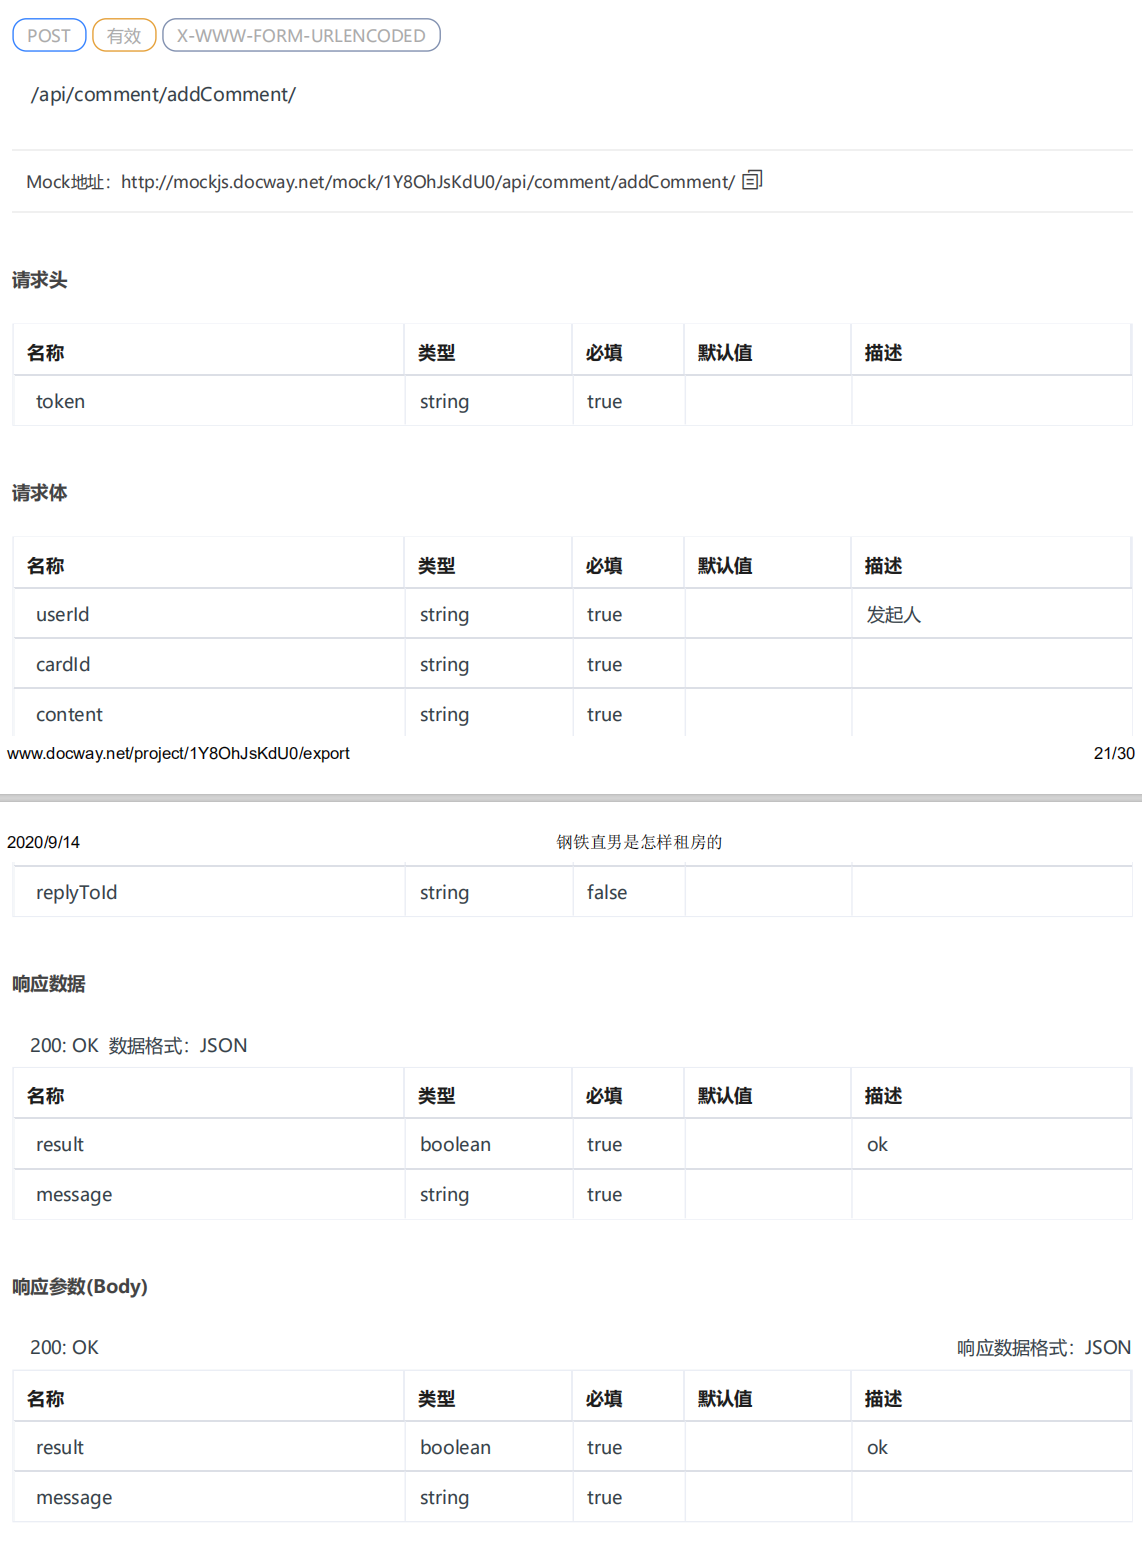
\includegraphics[height=19.0cm,width=14.0cm]{design/image/api23.png} 
            \end{figure}  
            \newpage 
            
        \subsubsection{删除评论} 
        \begin{figure}[h]
            \centering
            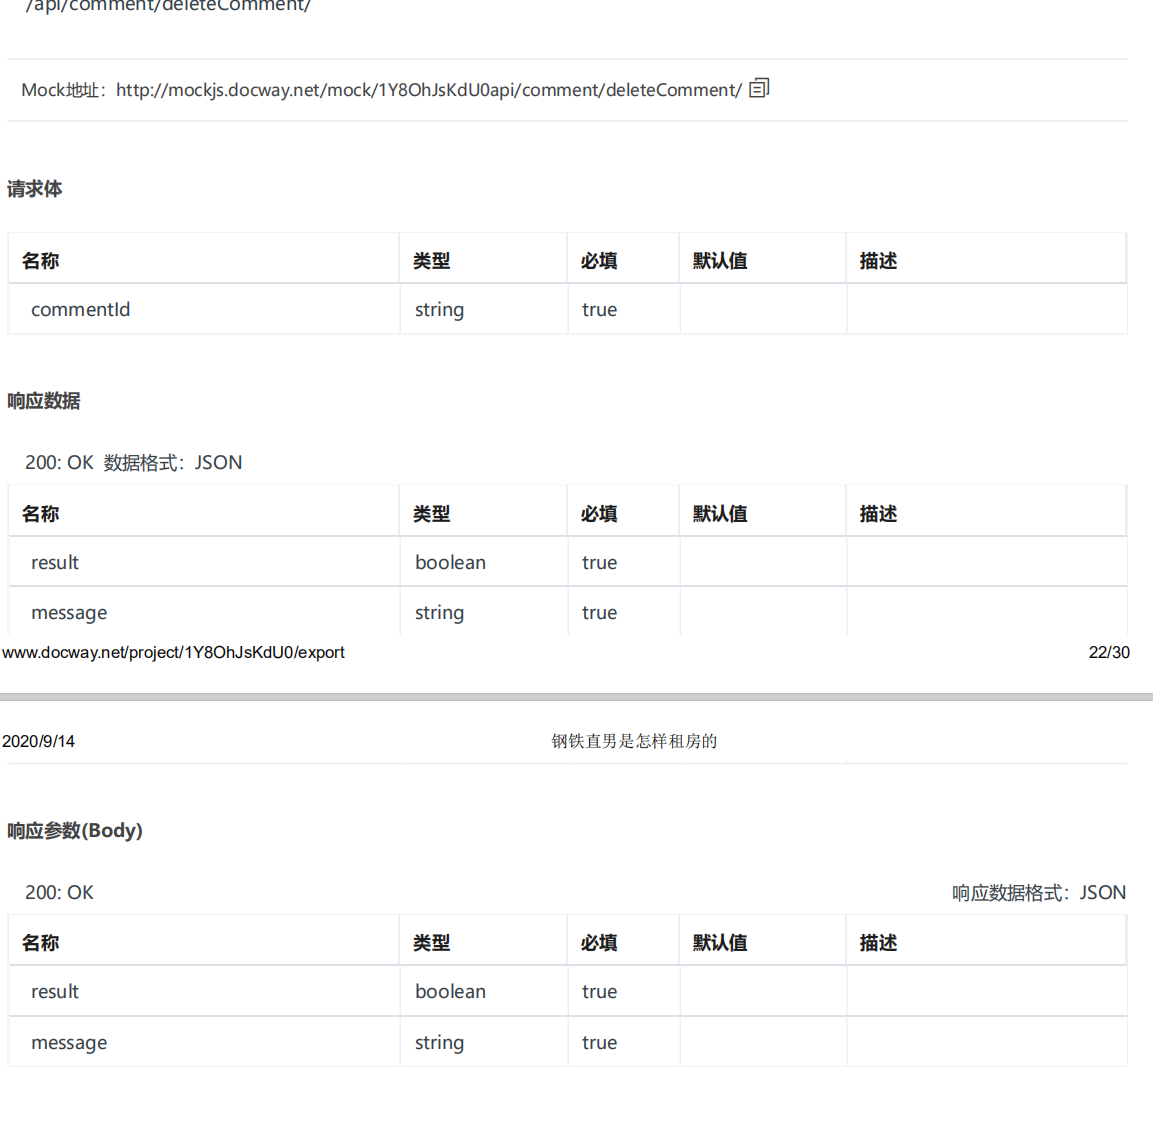
\includegraphics[height=19.0cm,width=14.0cm]{design/image/api24.png} 
            \end{figure}  
            \newpage  
            
        \subsection{发布}
     
        \subsubsection{发布资源}  
        \begin{figure}[h]
            \centering
            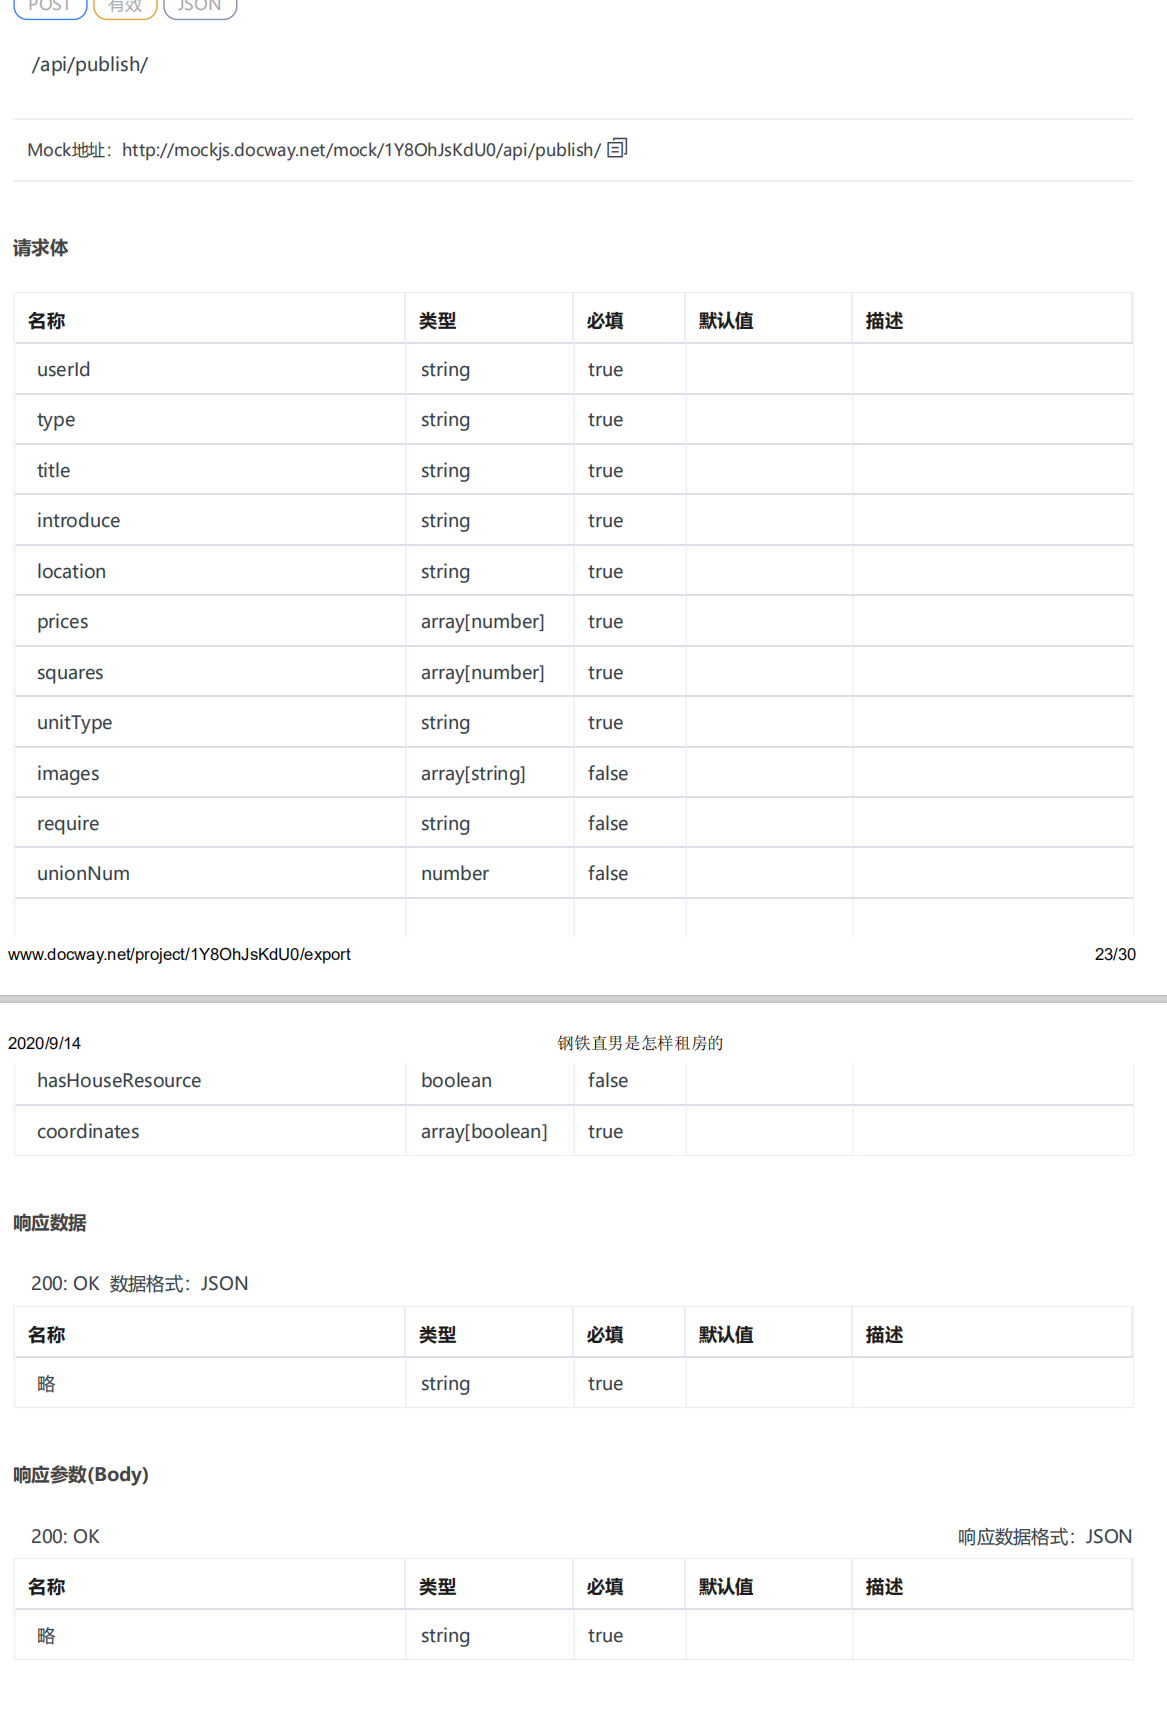
\includegraphics[height=19.0cm,width=14.0cm]{design/image/api25.png} 
            \end{figure}  
            \newpage  
        \subsubsection{上传图片文件返回链接}
        \begin{figure}[h]
            \centering
            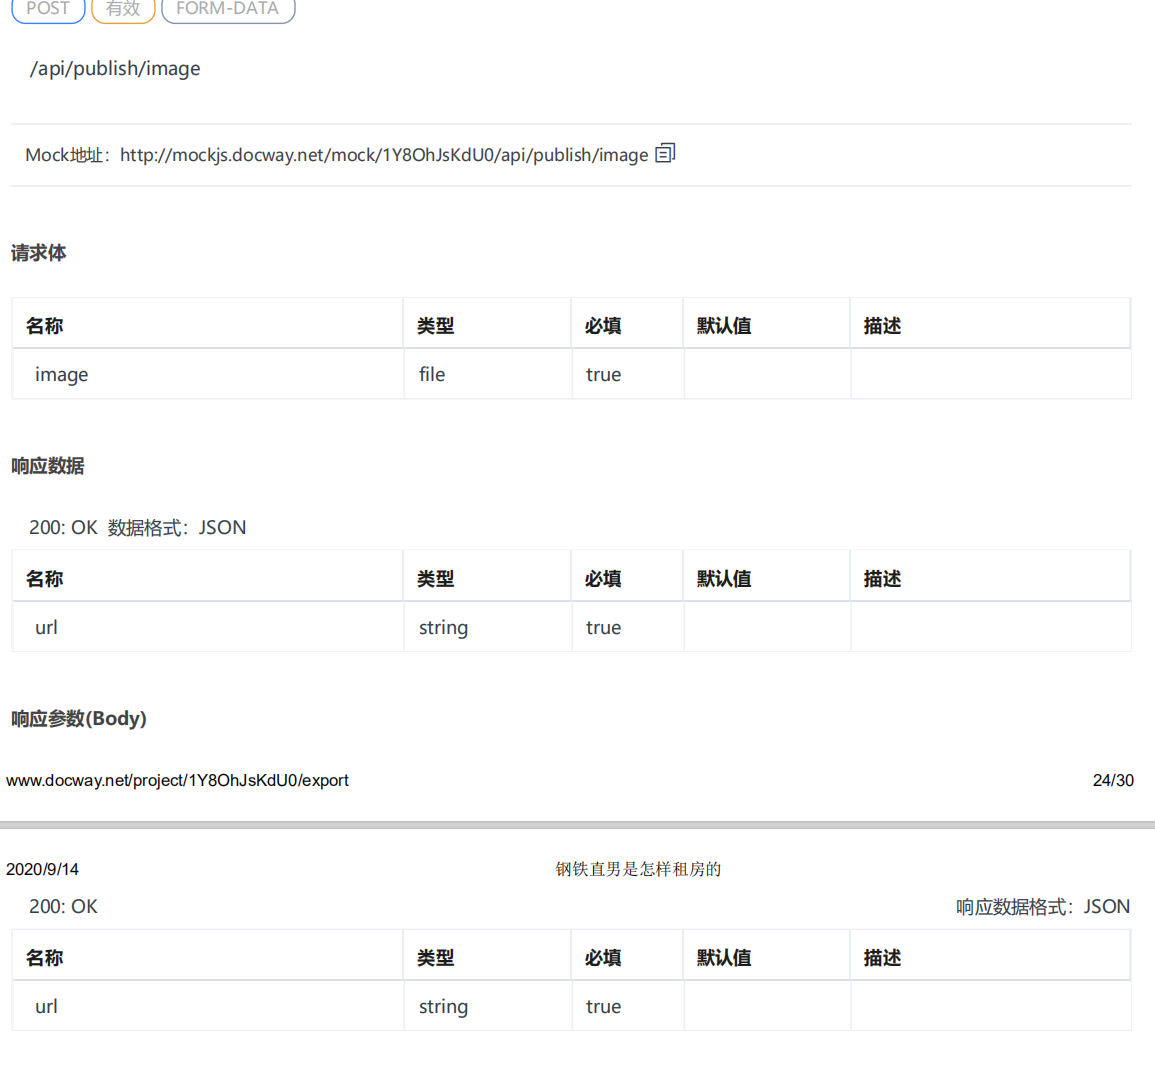
\includegraphics[height=16.0cm,width=14.0cm]{design/image/api26.png} 
            \end{figure}  
            \newpage
        \subsection{个人信息}
        \subsubsection{获取个人信息}
        \begin{figure}[h]
            \centering
            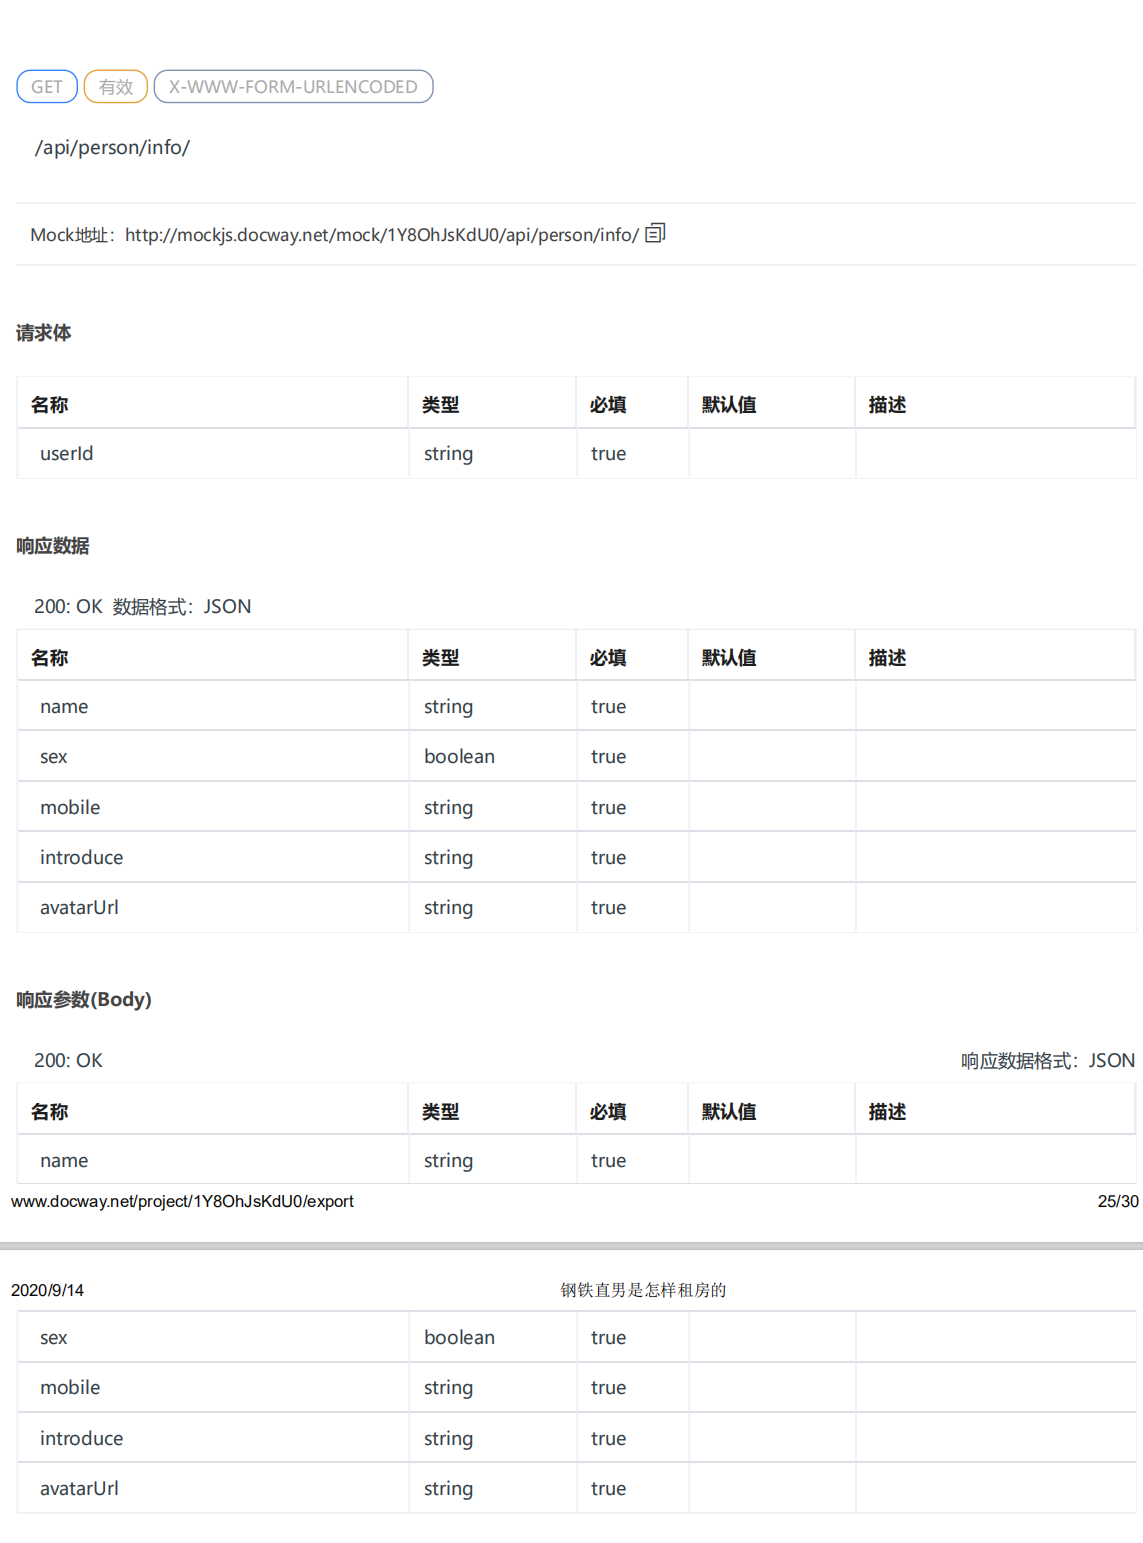
\includegraphics[height=19.0cm,width=14.0cm]{design/image/api27.png} 
            \end{figure}  
            \newpage
         \subsubsection{修改个人信息}     
         \begin{figure}[h]
            \centering
            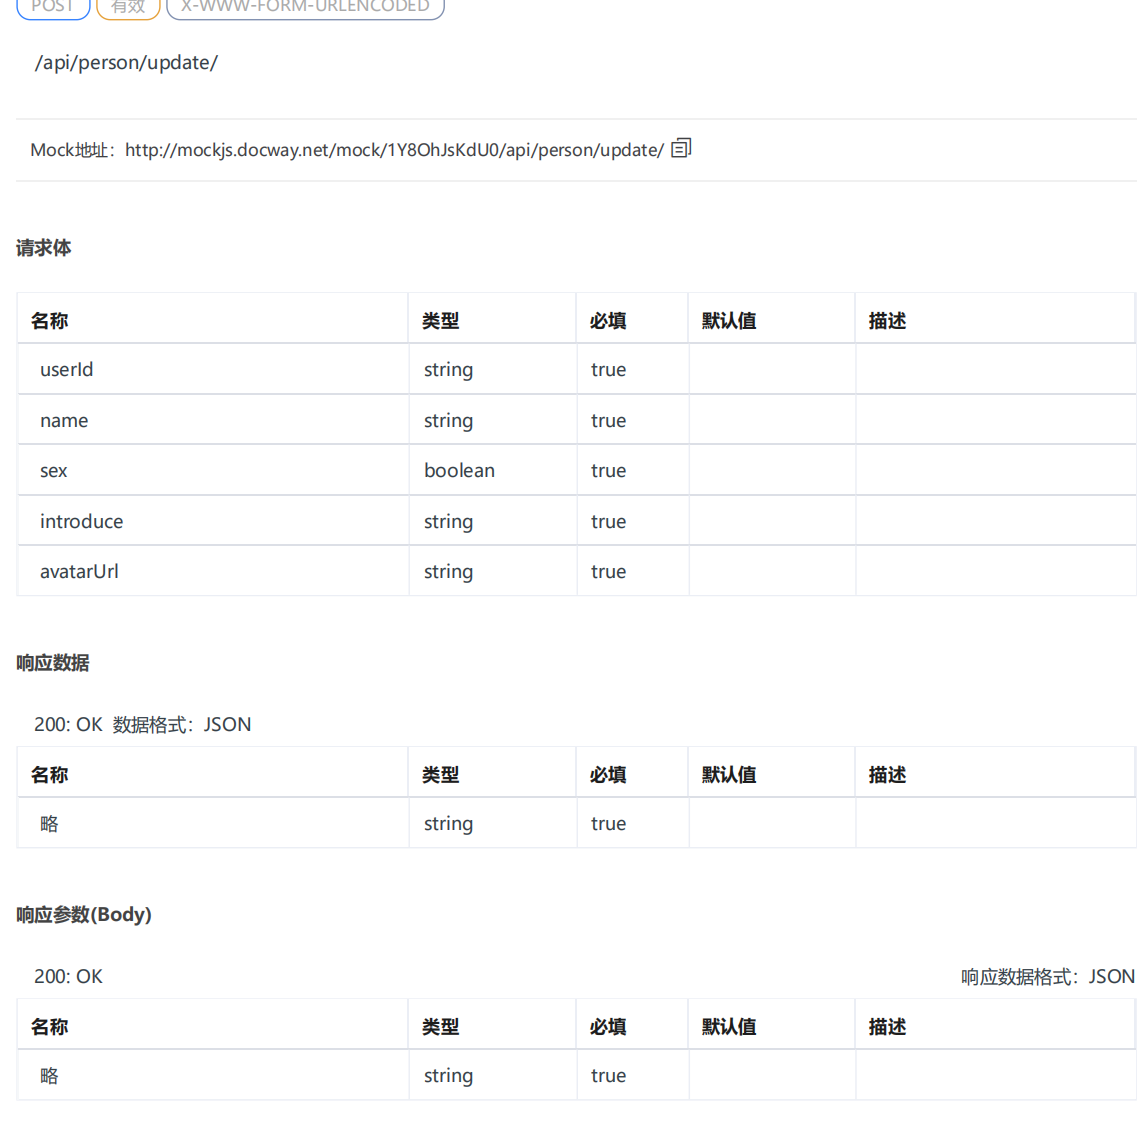
\includegraphics[height=17.0cm,width=14.0cm]{design/image/api28.png} 
            \end{figure}  
            \newpage
        \subsection{消息列表}

        \subsubsection{获取消息列表}
        \begin{figure}[h]
            \centering
            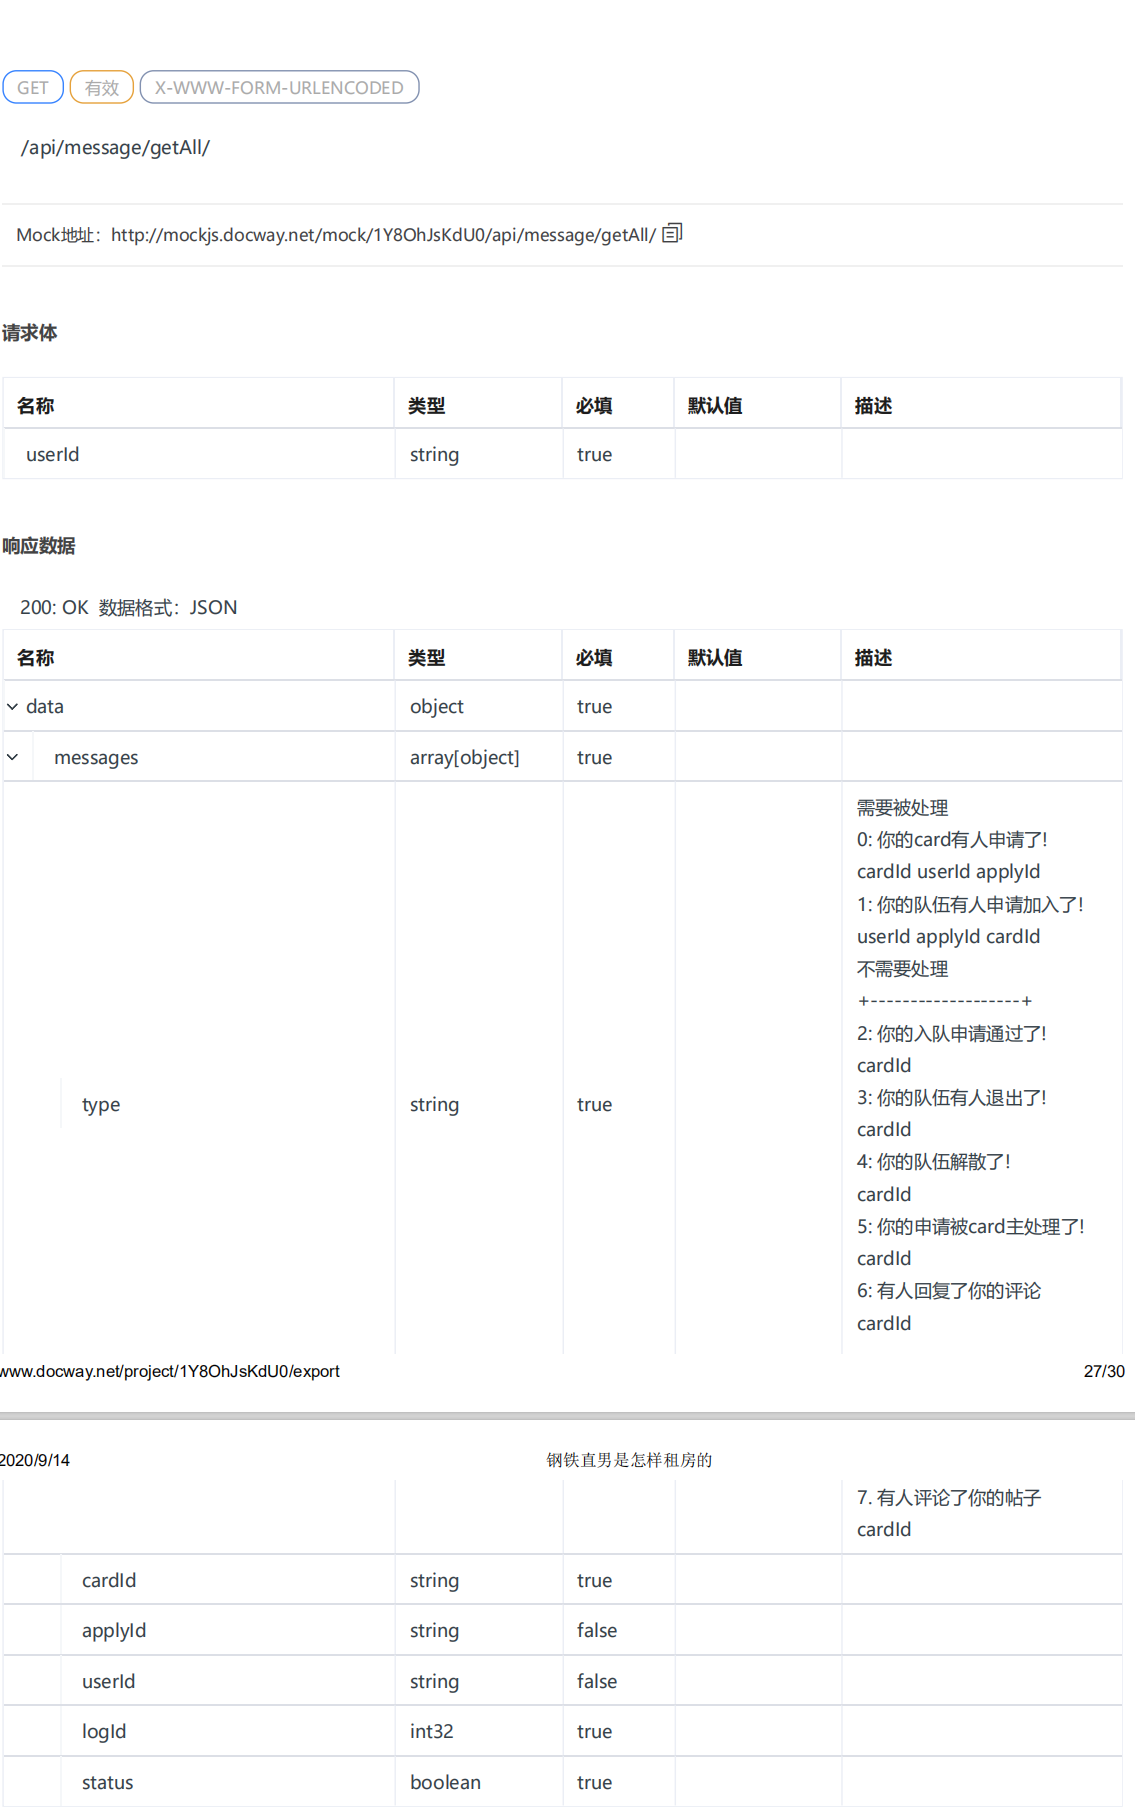
\includegraphics[height=19.0cm,width=14.0cm]{design/image/api29.png} 
            \end{figure}  
            \newpage
            \begin{figure}[h]
                \centering
                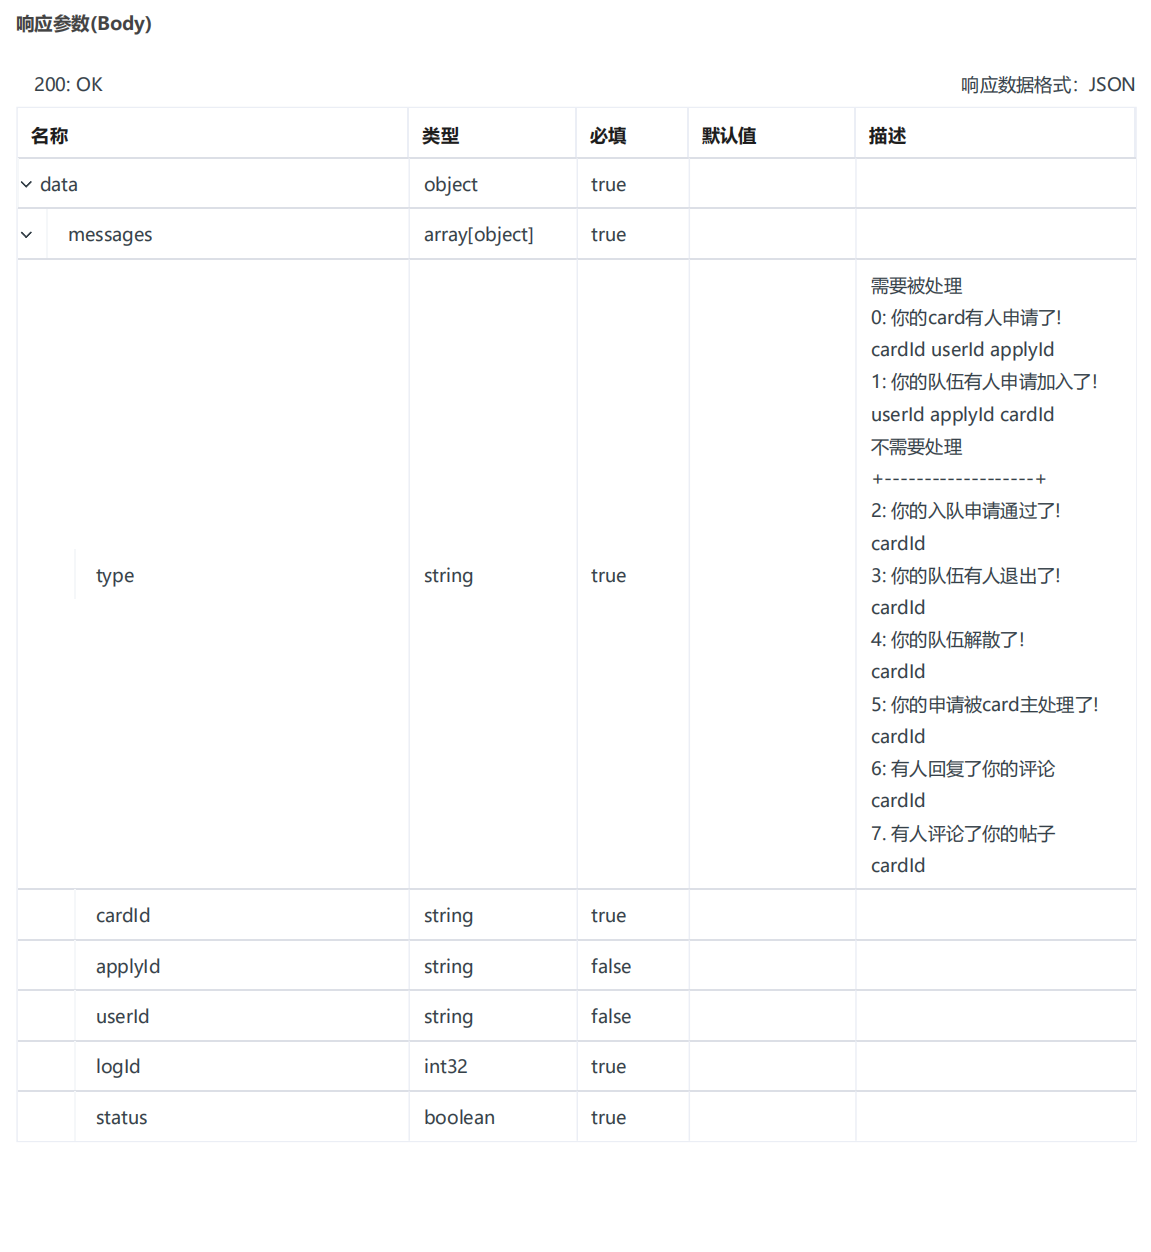
\includegraphics[height=19.0cm,width=14.0cm]{design/image/api30.png} 
                \end{figure}  
                \newpage
        \subsection{已完成订单}        
        \subsubsection{获取所有已完成订单}
        \begin{figure}[h]
            \centering
            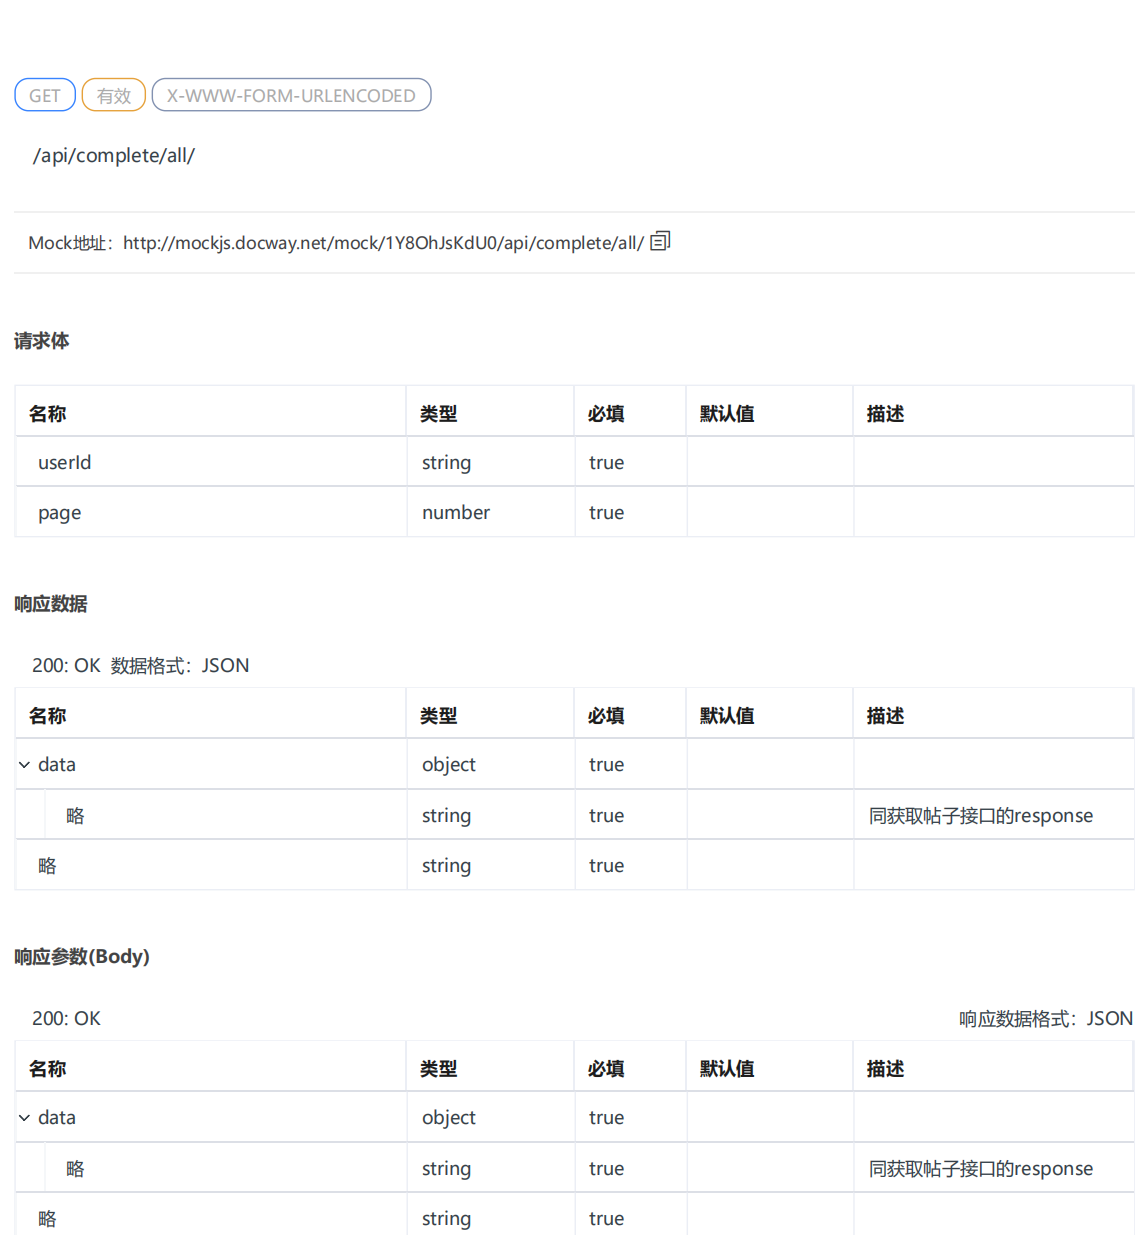
\includegraphics[height=19.0cm,width=14.0cm]{design/image/api31.png} 
            \end{figure}  
            \newpage
        \subsection{未完成订单}        
        \subsubsection{获取所有未完成订单}
        \begin{figure}[h]
            \centering
            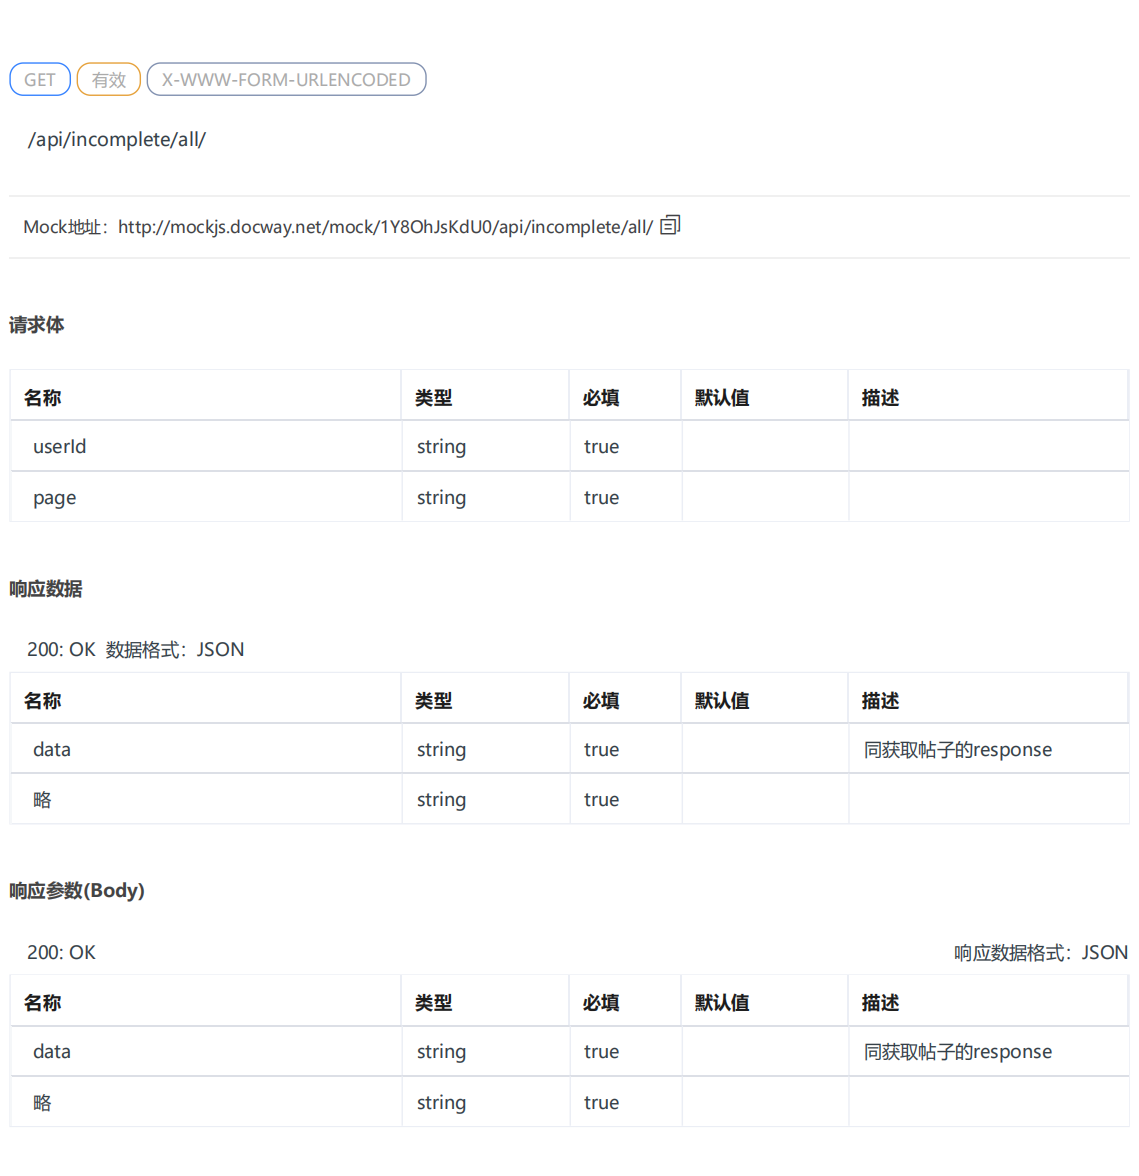
\includegraphics[height=19.0cm,width=14.0cm]{design/image/api32.png} 
            \end{figure}  
            \newpage
\section{管理员API设计}
\href{https://documentation-1303131952.cos.ap-beijing.myqcloud.com/iron_man/%E7%AE%A1%E7%90%86%E5%91%98API%E6%96%87%E6%A1%A3.pdf}{点击查看 管理员API设计文档}
\subsection{登录}
\subsubsection{管理员登陆}
\begin{figure}[h]
    \centering
    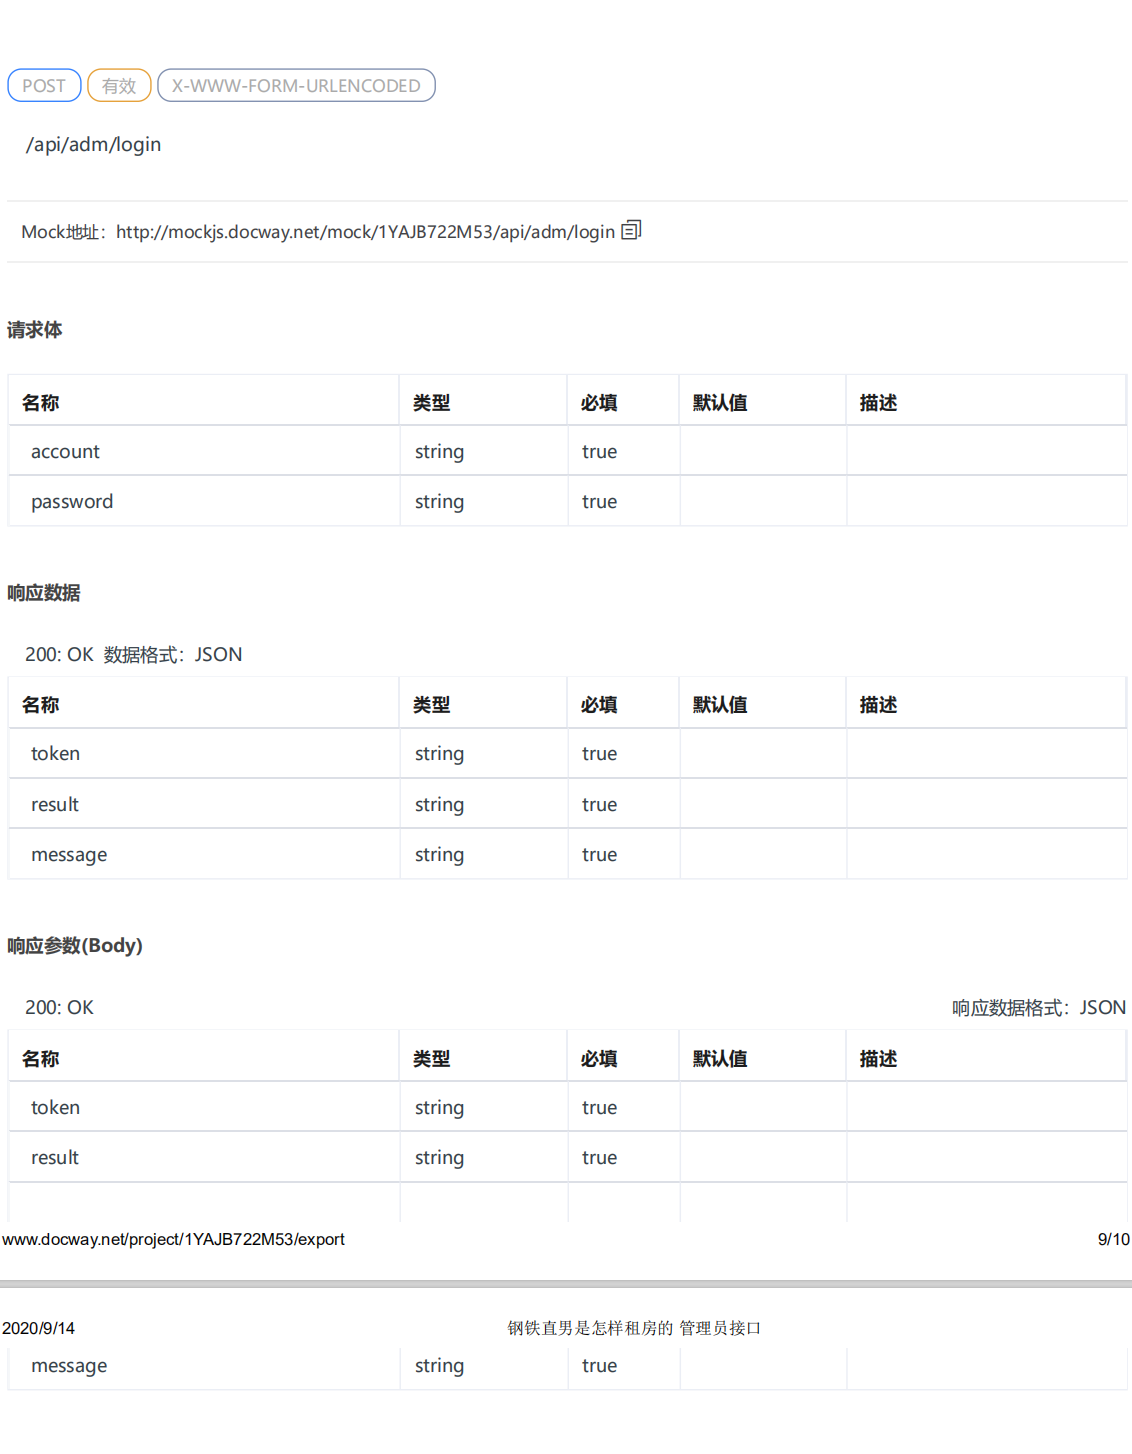
\includegraphics[height=18.0cm,width=14.0cm]{design/image/api33.png} 
    \end{figure}  
    \newpage
\subsection{帖子管理}
\subsubsection{查询符合条件的帖子}
\begin{figure}[h]
    \centering
    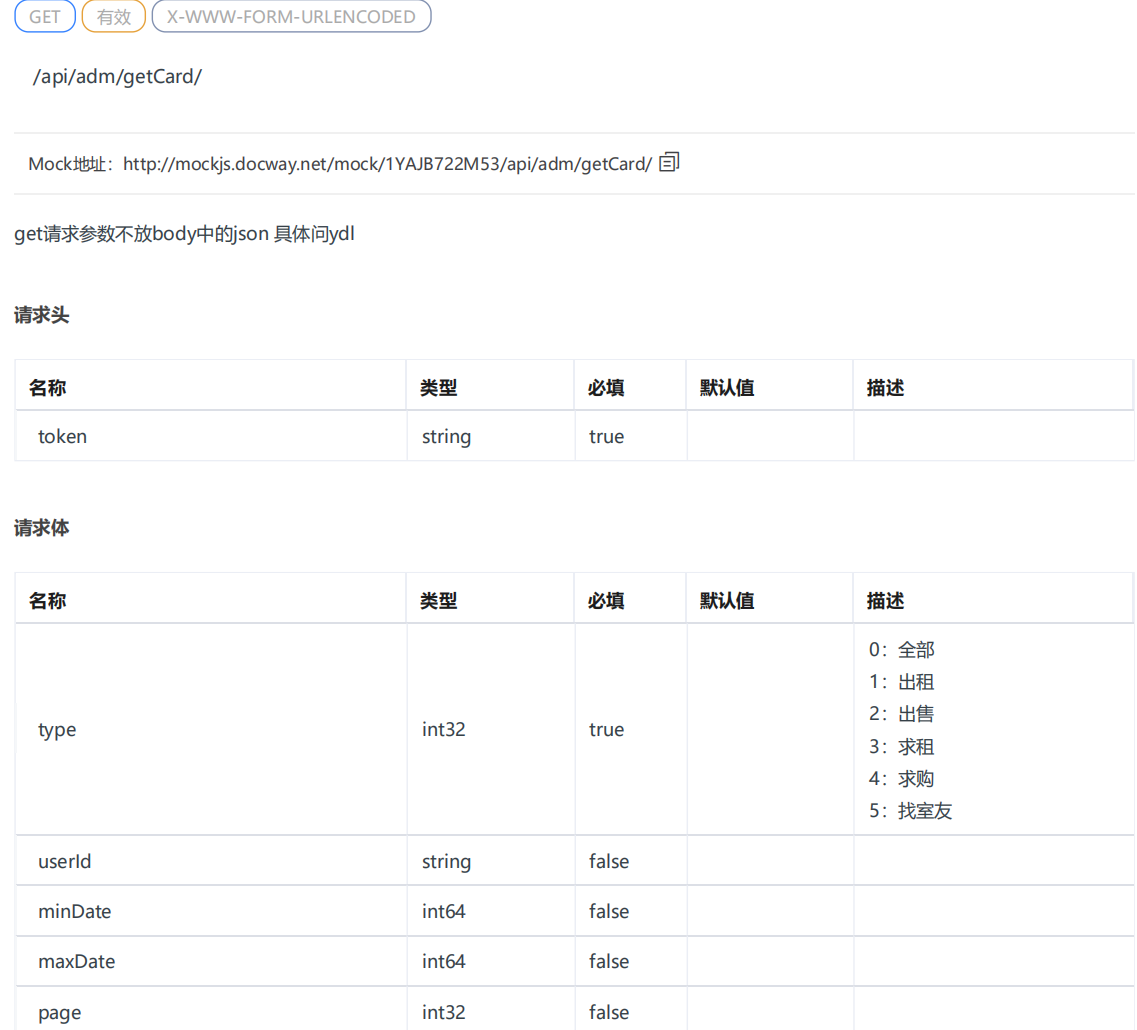
\includegraphics[height=16.5cm,width=14.0cm]{design/image/api34.png} 
    \end{figure}  
    \newpage
    \begin{figure}[h]
        \centering
        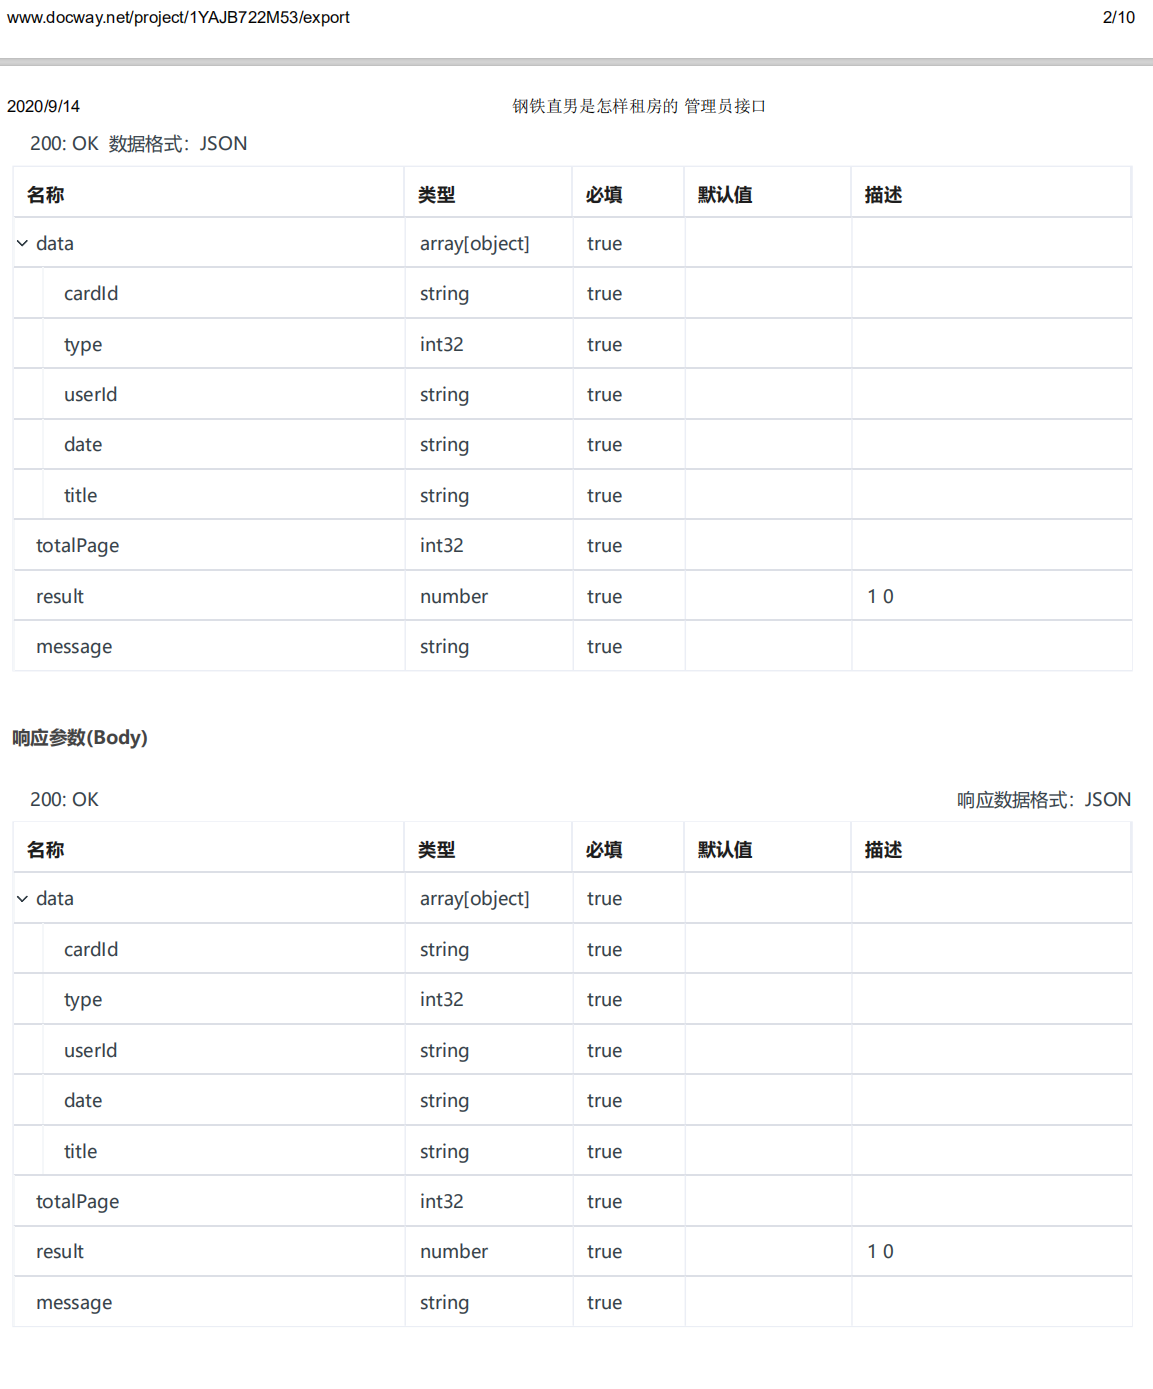
\includegraphics[height=19.0cm,width=14.0cm]{design/image/api35.png} 
        \end{figure}  
        \newpage
\subsubsection{查询帖子详情}
\begin{figure}[h]
    \centering
    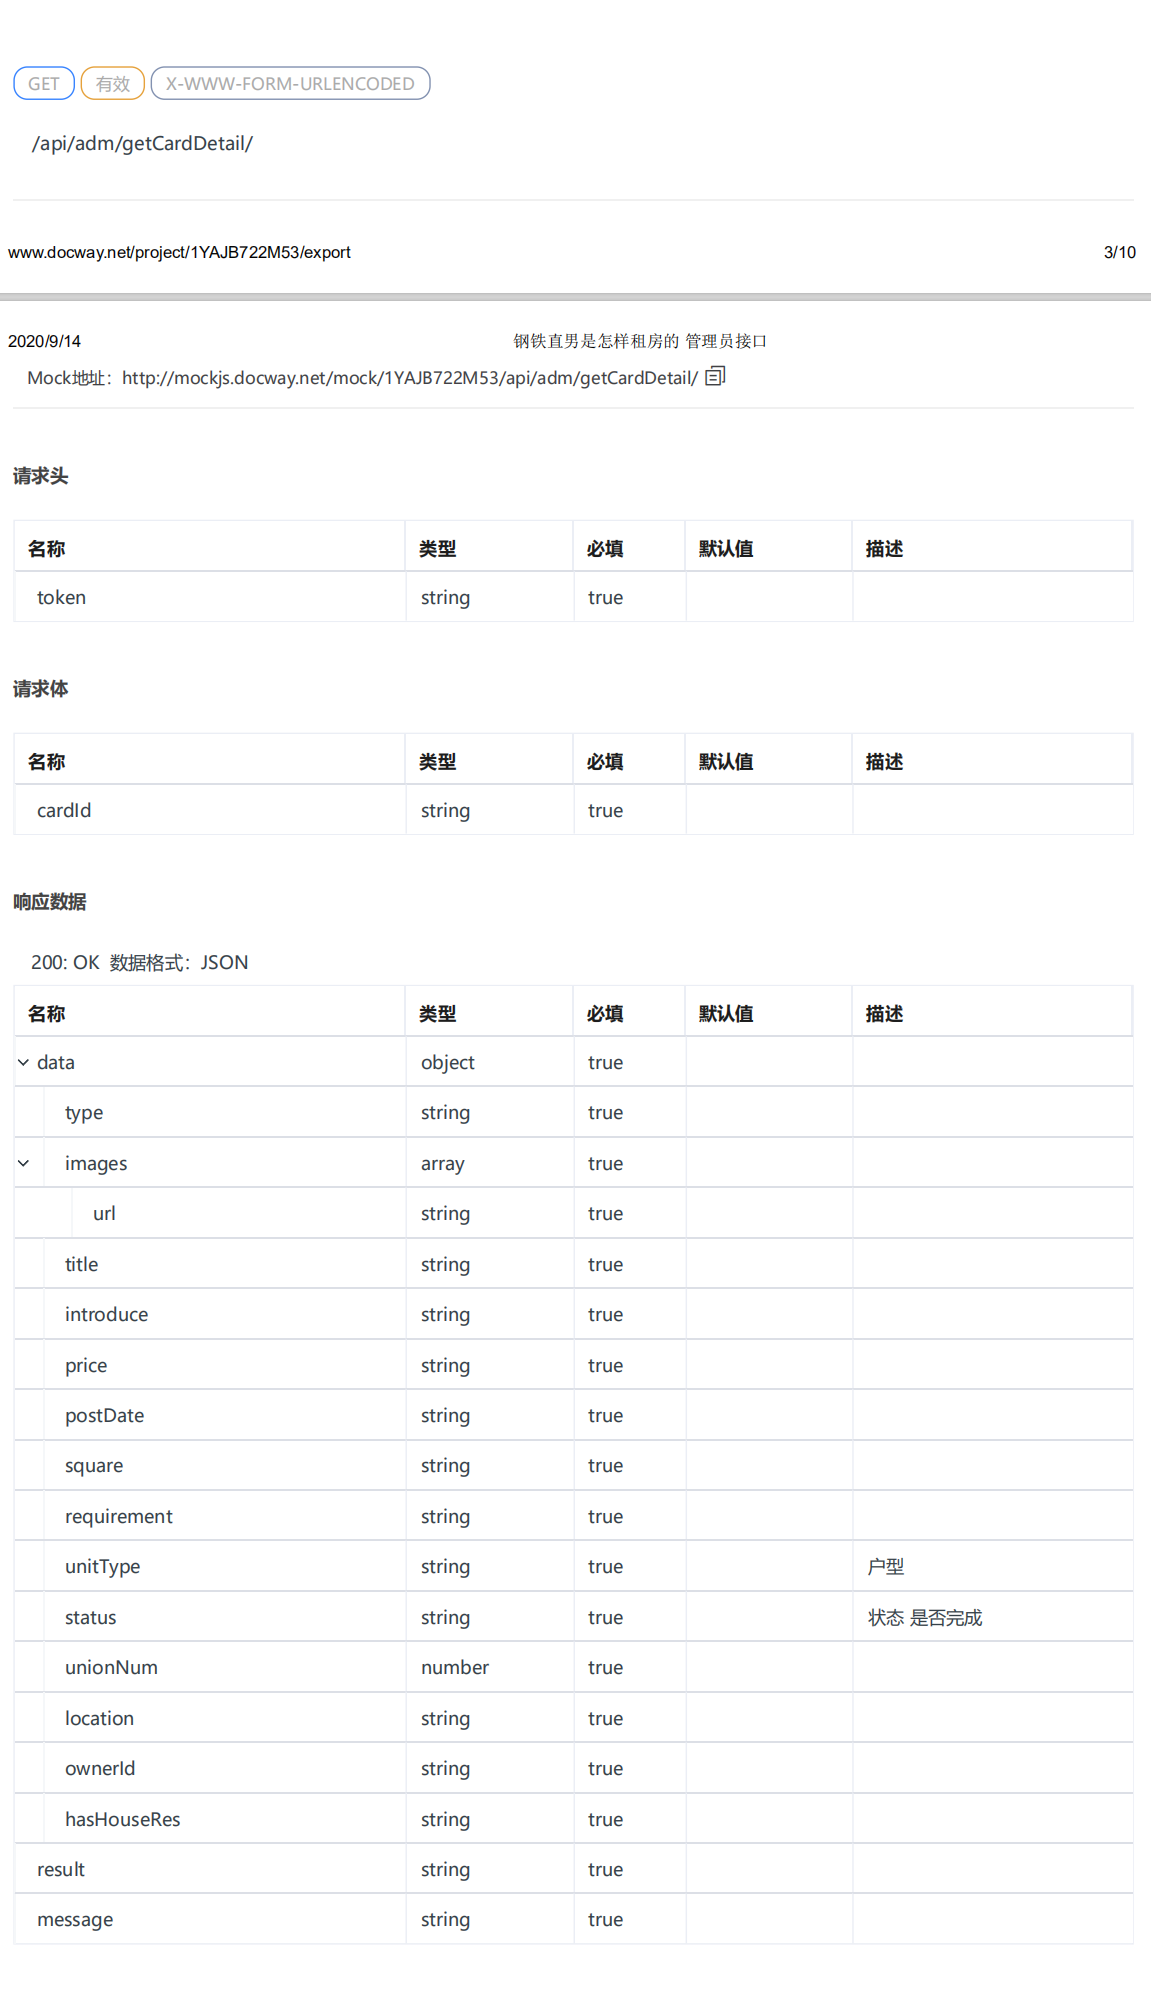
\includegraphics[height=19.0cm,width=14.0cm]{design/image/api36.png} 
    \end{figure}  
    \newpage
    \begin{figure}[h]
        \centering
        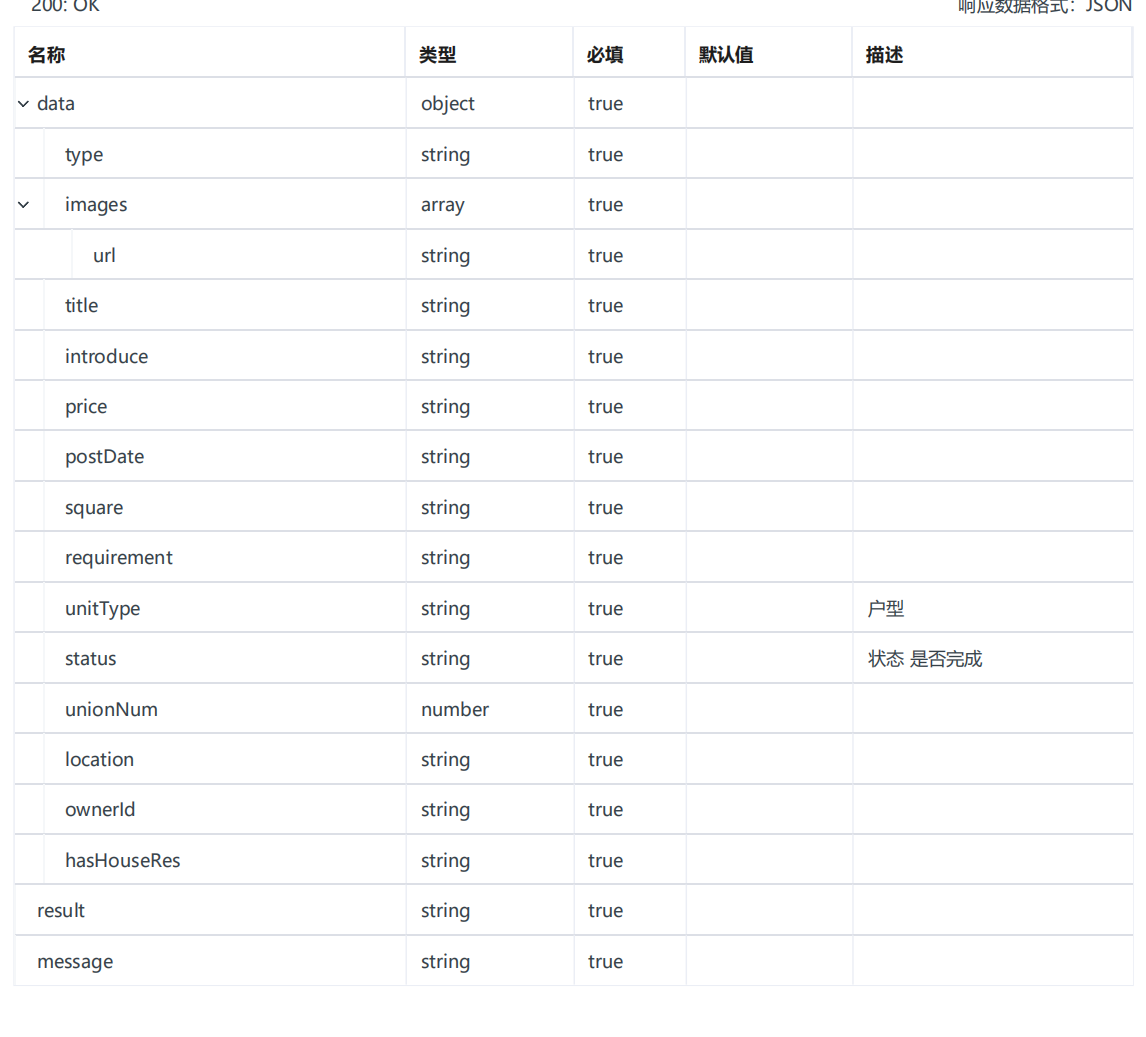
\includegraphics[height=19.0cm,width=14.0cm]{design/image/api37.png} 
        \end{figure}  
        \newpage
\subsubsection{批量删除帖子}
\begin{figure}[h]
    \centering
    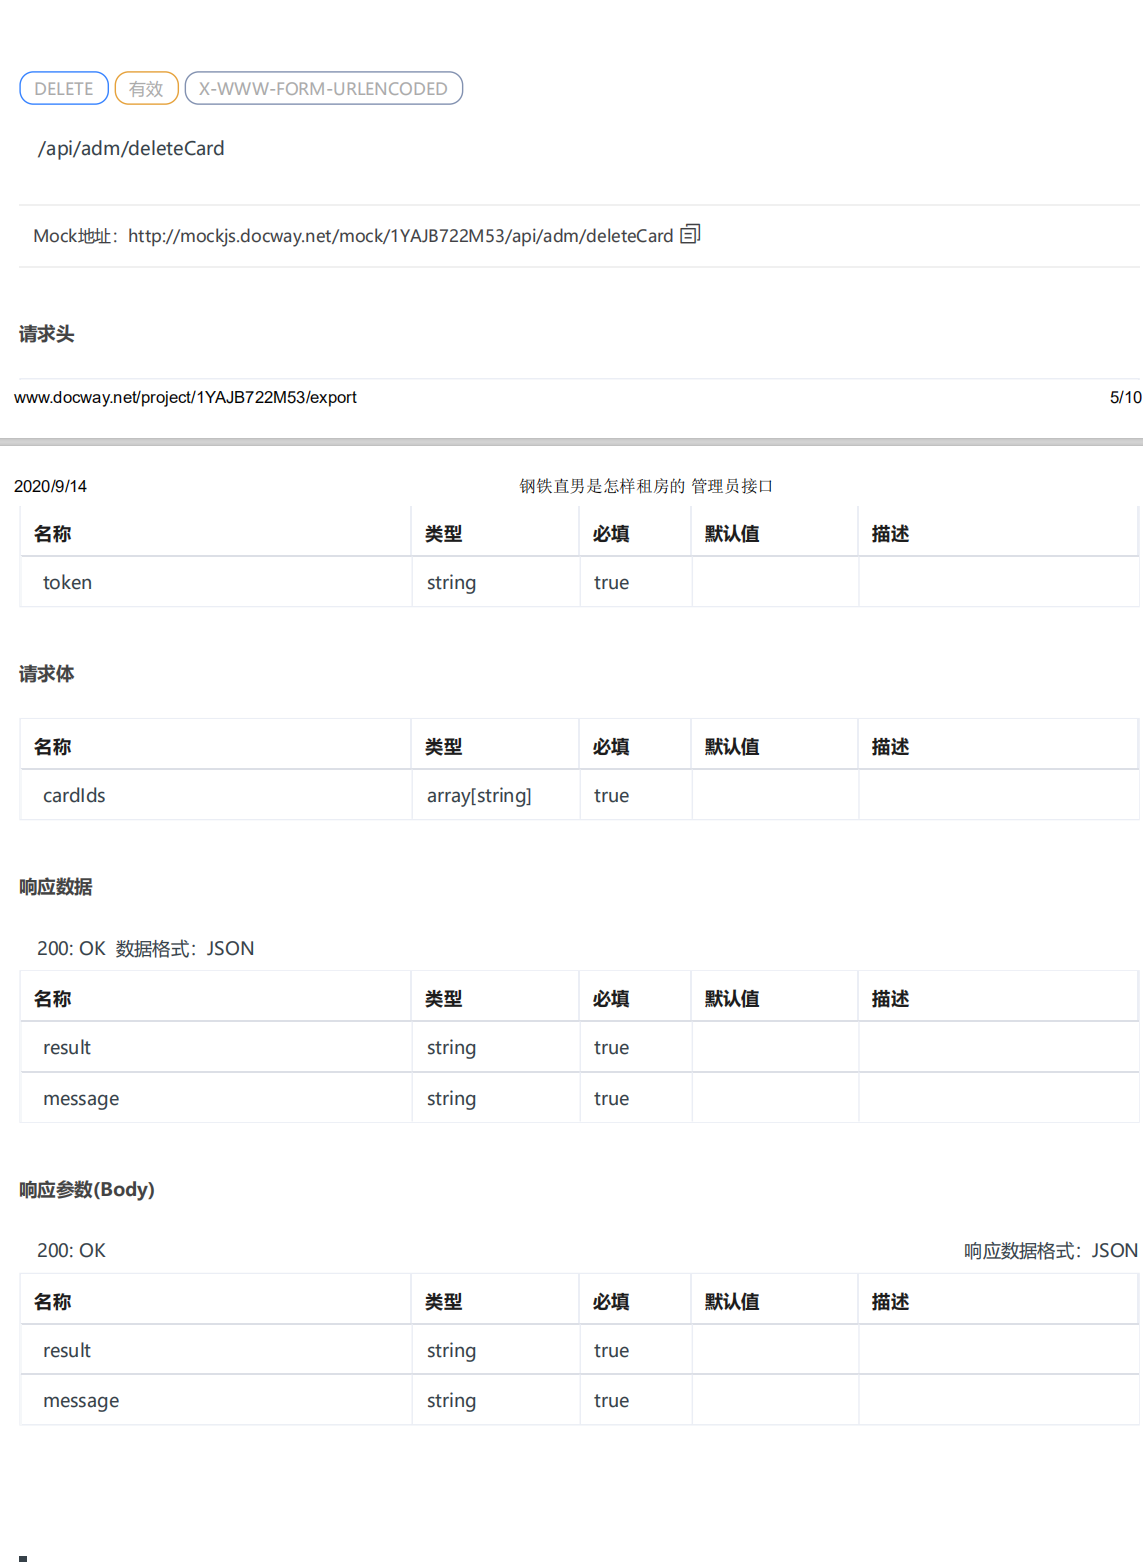
\includegraphics[height=19.0cm,width=14.0cm]{design/image/api38.png} 
    \end{figure}  
    \newpage

\subsection{用户管理}

\subsubsection{查询符合条件的用户}
\begin{figure}[h]
    \centering
    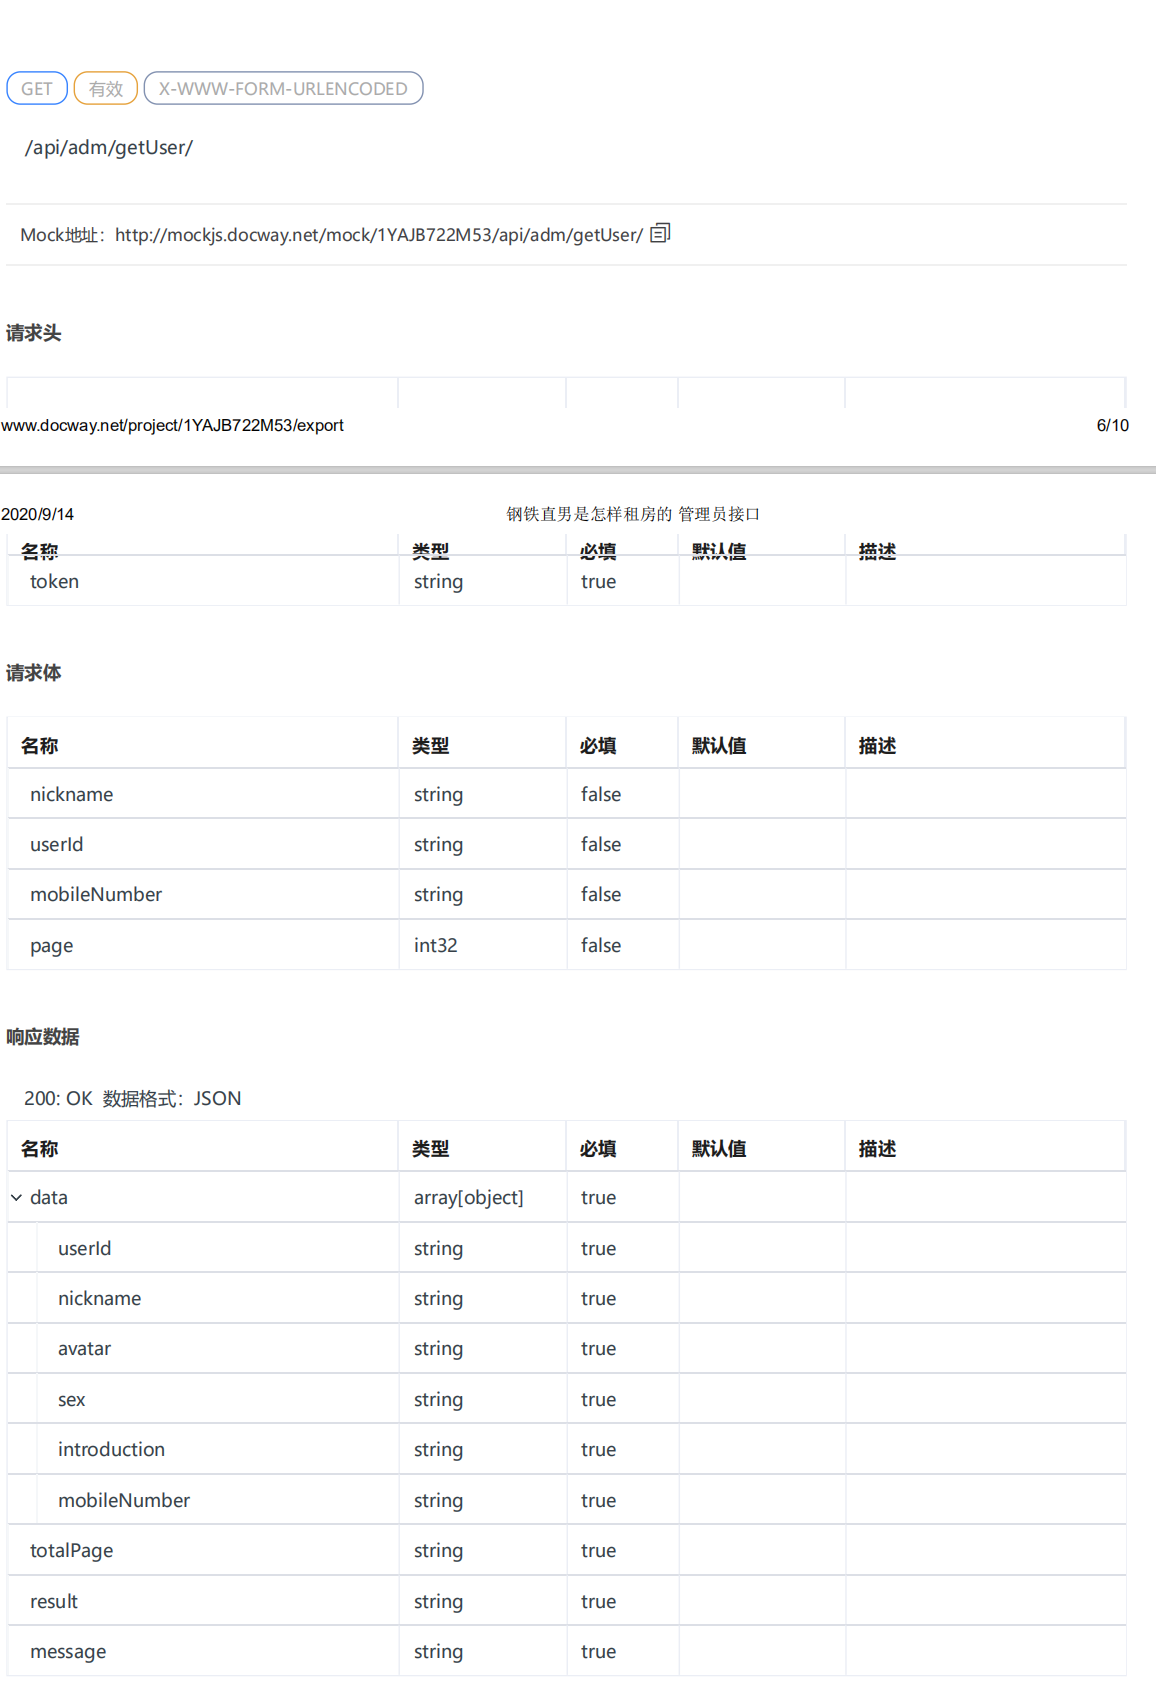
\includegraphics[height=19.0cm,width=14.0cm]{design/image/api39.png} 
    \end{figure}  
    \newpage
    \begin{figure}[h]
        \centering
        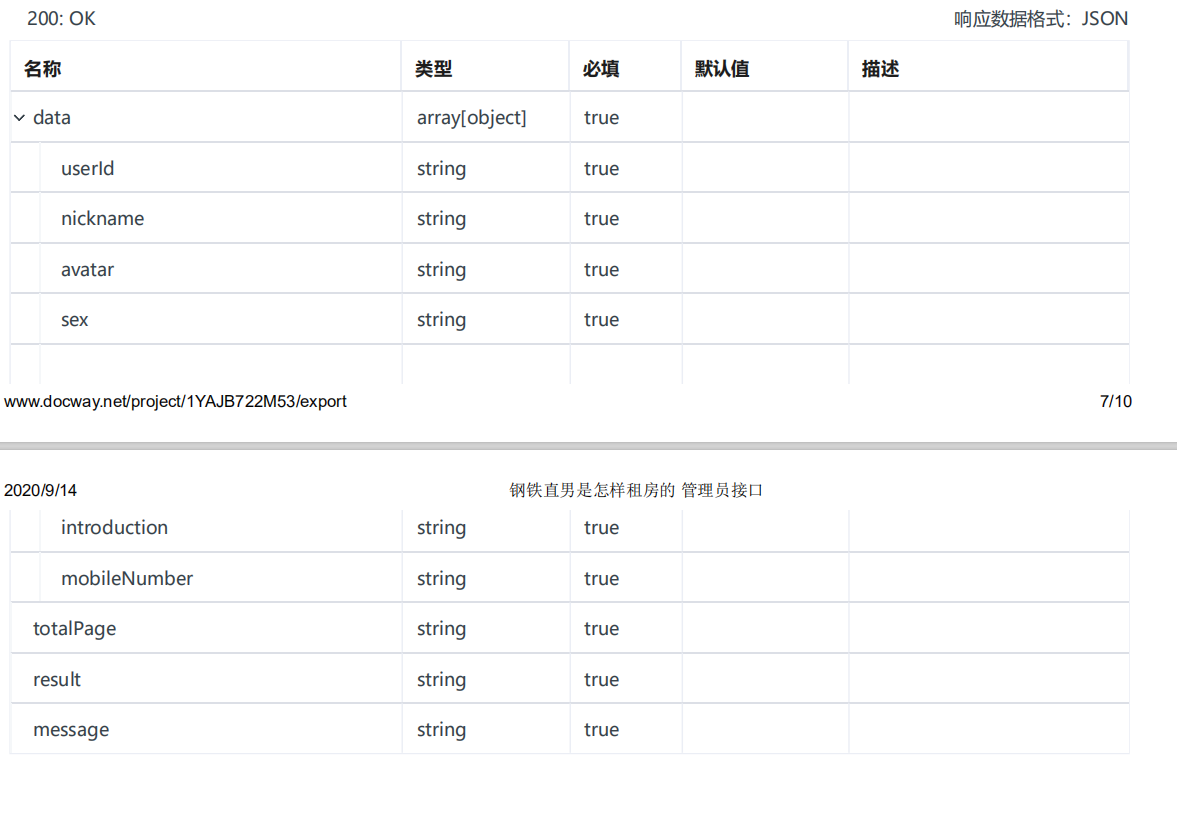
\includegraphics[height=15.0cm,width=14.0cm]{design/image/api40.png} 
        \end{figure}  
        \newpage
    
\subsubsection{删除指定用户}

\begin{figure}[h]
    \centering
    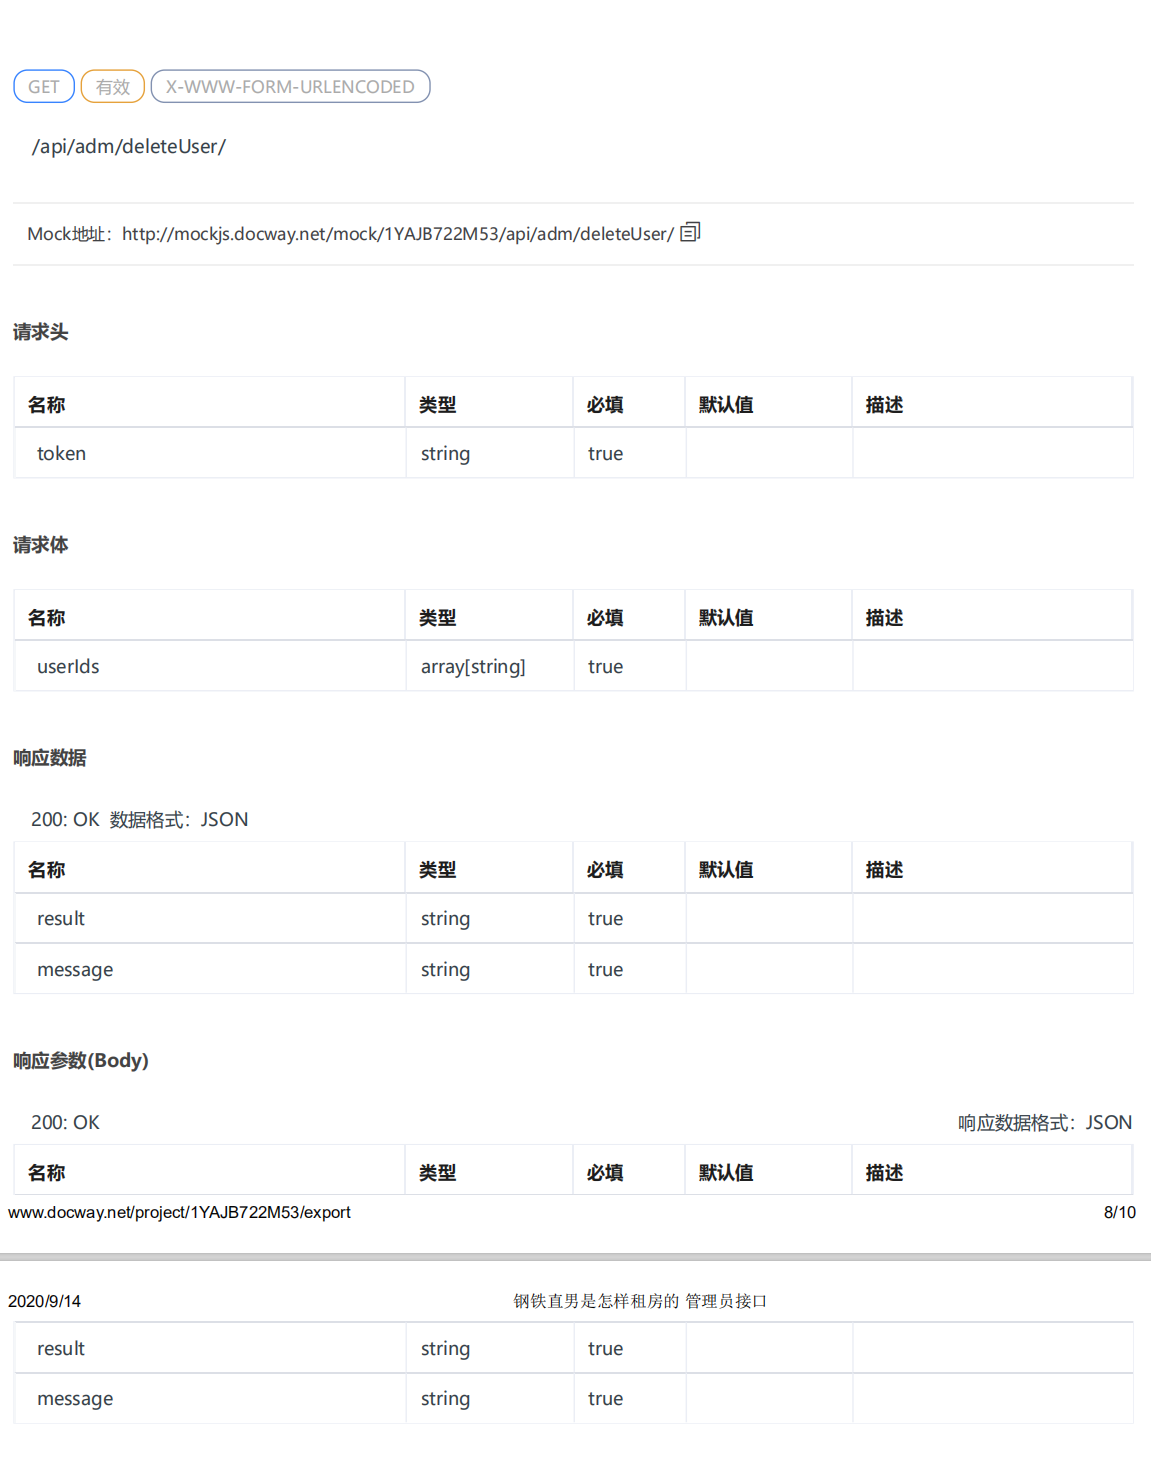
\includegraphics[height=19.0cm,width=14.0cm]{design/image/api41.png} 
    \end{figure}  
    \newpage
	\chapter{数据库设计(E/R图)}

\href{https://documentation-1303131952.cos.ap-beijing.myqcloud.com/iron_man/%E6%95%B0%E6%8D%AE%E5%BA%93%E8%AE%BE%E8%AE%A1%E5%9B%BE.png}{点击查看 E/R 图}

\begin{figure}[h]
    \centering
    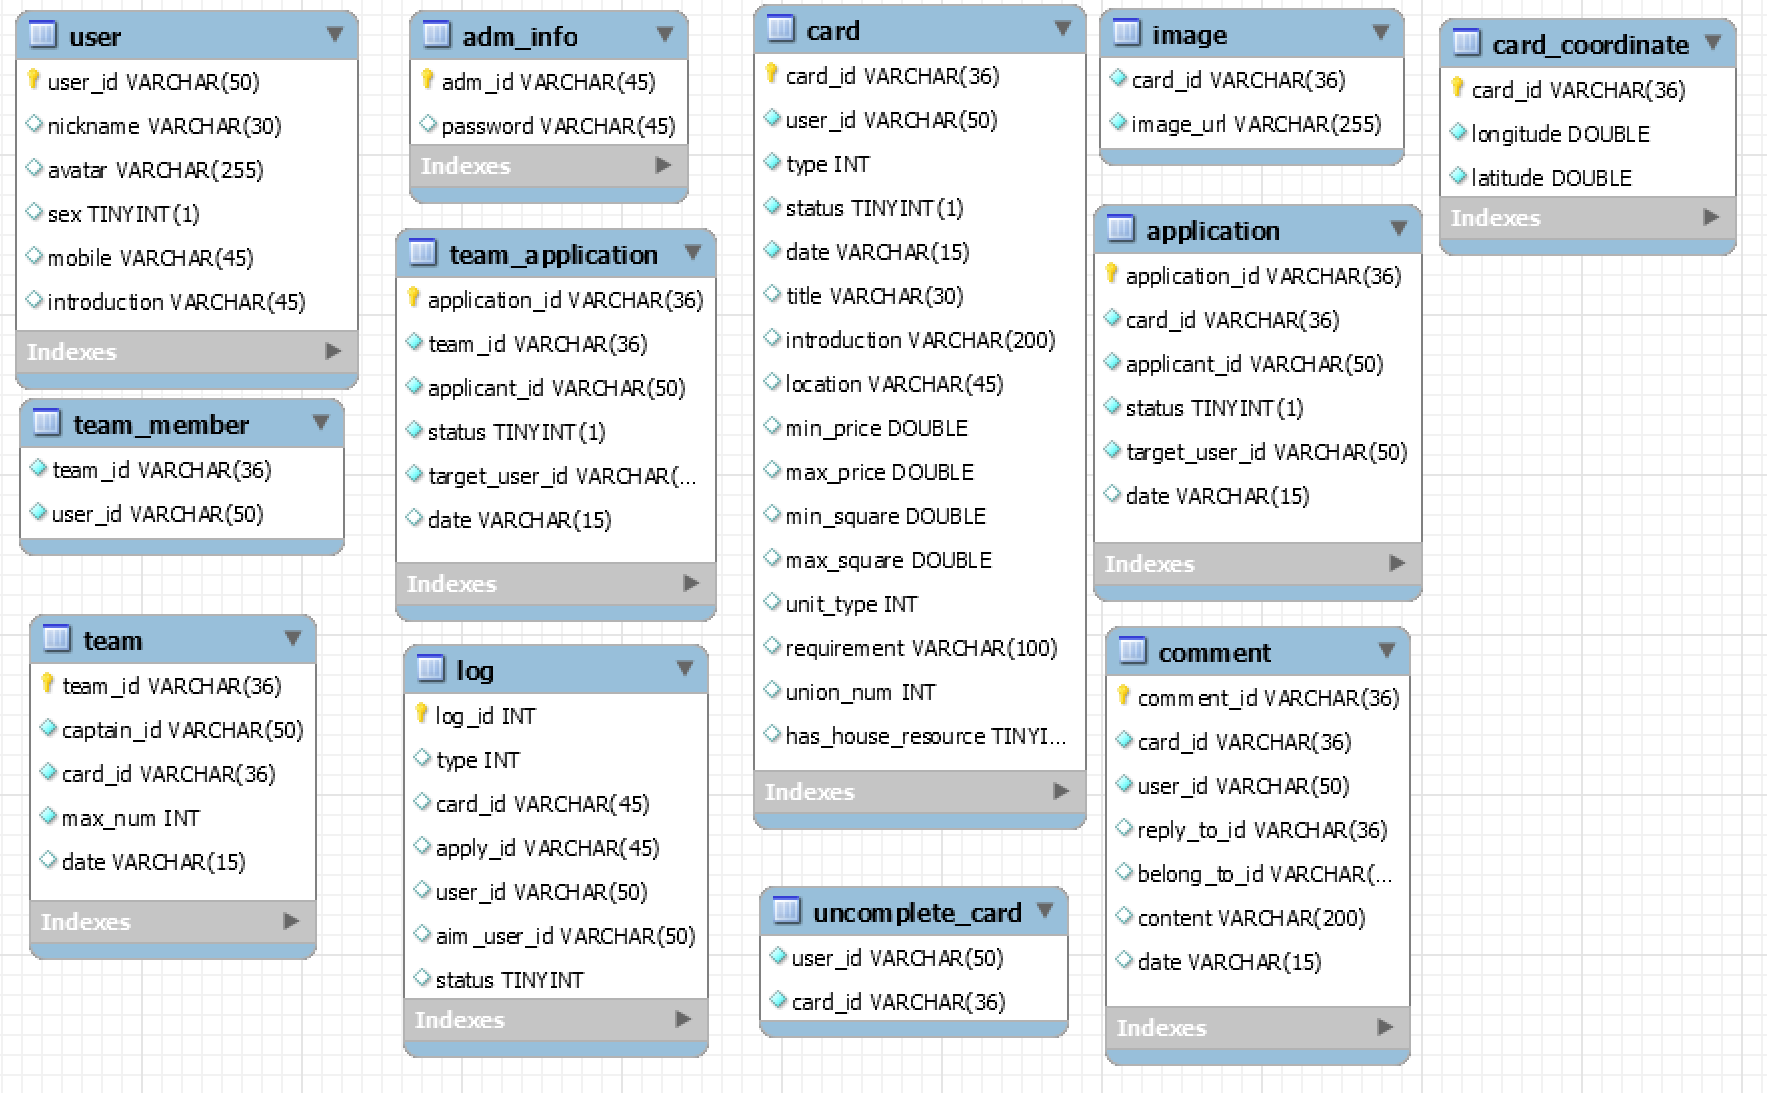
\includegraphics[height=11.0cm,width=14.0cm]{design/image/er.png} 
    \end{figure}
\newpage
	\chapter{结构设计}

\section{软件体系结构图}

\begin{figure}[h]
\centering
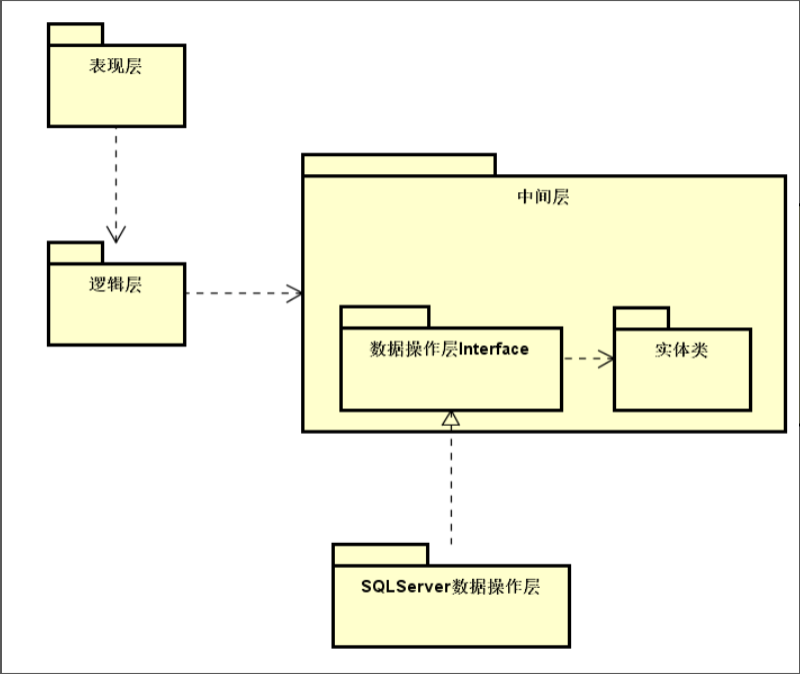
\includegraphics[height=11.0cm,width=14.0cm]{design/image/tixi.png}
\end{figure}
\newpage
\section{类设计图}

\href{https://documentation-1303131952.cos.ap-beijing.myqcloud.com/iron_man/%E7%B1%BB%E5%9B%BE.svg}{点击查看 类图}

\begin{figure}[h]
    \centering
    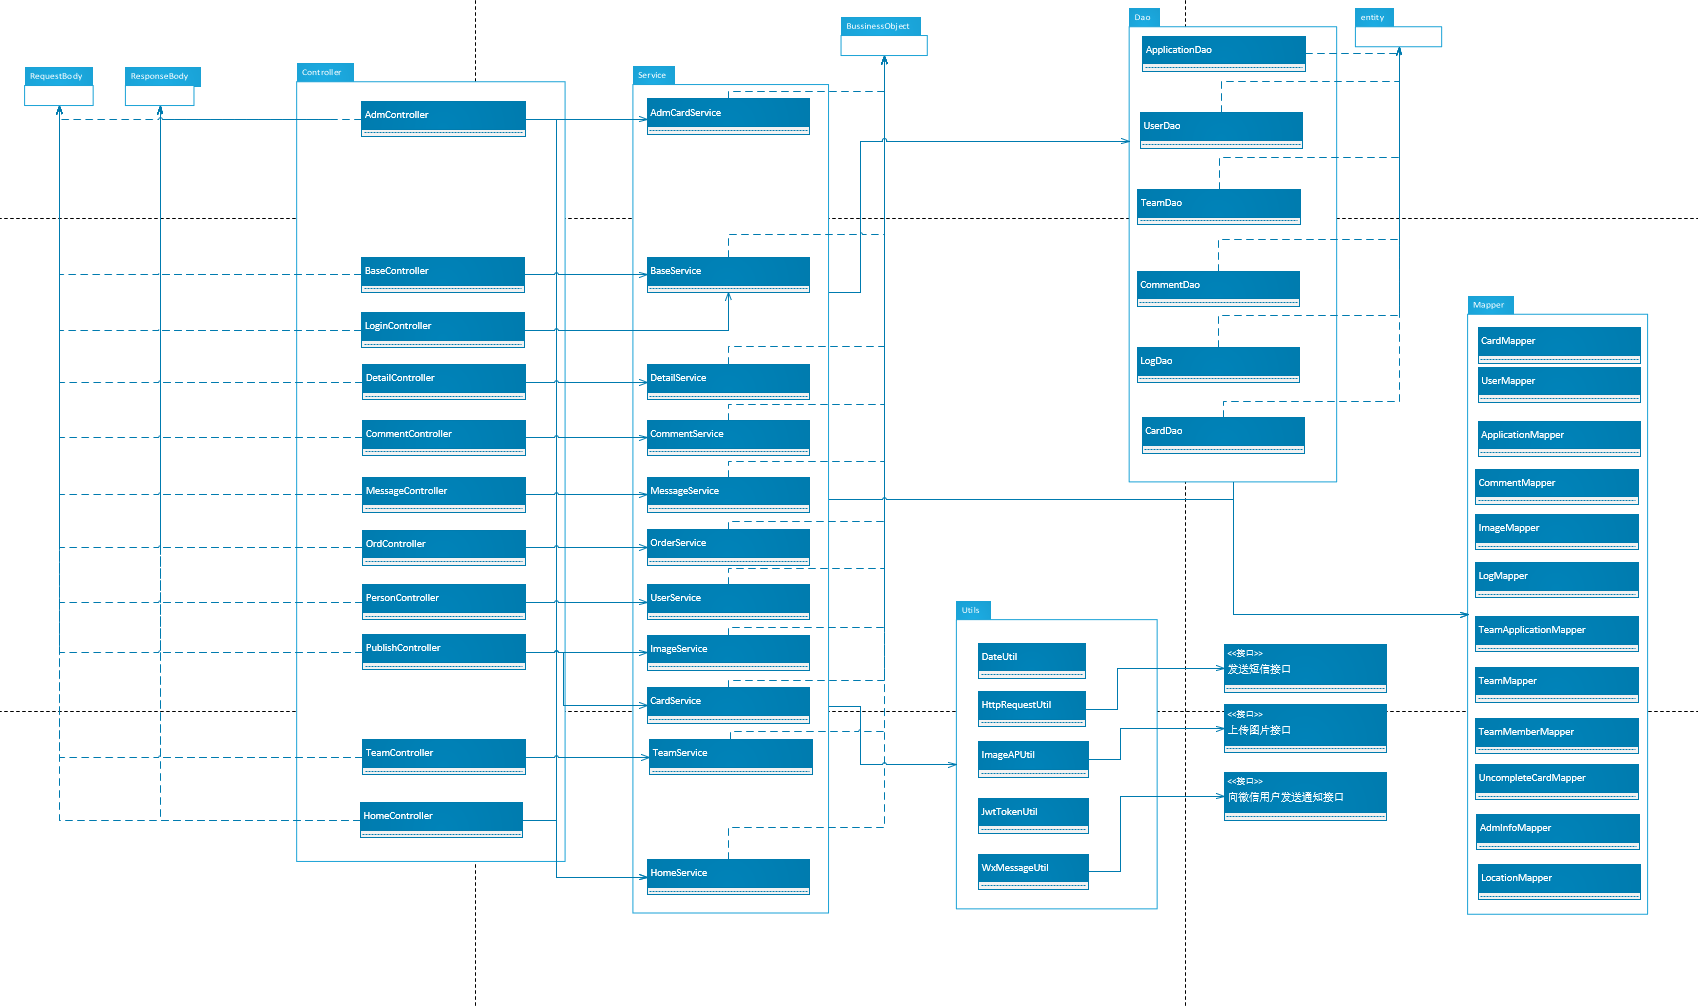
\includegraphics[height=11.0cm,width=14.0cm]{design/image/class.png} 
    \end{figure}
    \newpage    
	\definecolor{keywordcolor}{rgb}{0.8,0.1,0.5}
\definecolor{webgreen}{rgb}{0,.5,0}
\lstset{language=[AspectJ]Java,
basicstyle=\footnotesize,
keywordstyle=\color{keywordcolor}\bfseries, %\underbar,
identifierstyle=,
commentstyle=\color{blue} \textit,
stringstyle=\ttfamily,
showstringspaces=false,
captionpos=b
}
\chapter{类设计}

\section{Controller设计}

\subsection{AdmController}

1. 功能: 接收管理员端发出的http请求,并返回相应的数据 \\
2. 方法定义
\begin{lstlisting}
    /**
    * 获取全部的符合类型的帖子
    * GET /api/adm/getCard/
    */
    public GetCardResponse getCards(
        int type, 
        String userId, 
        Long minDate,
        Long maxDate, 
        int page);
    /**
    * 删除指定帖子
    * DELETE /api/adm/deleteCard/
    */
    public DefaultResponse deleteCards(
        DeleteCardsRequest deleteCardsRequest);
    /**
     * 获取帖子详情
     * GET /api/adm/getCardDetail/
     */
    public CardResponse getCards(
        int type,
        int page,
        String location,
        double minPrice,
        double maxPrice,
        double minSquare,
        double maxSquare,
        int unitType,
        boolean hasHouseResource);

  /**
   * 获取符合条件的用户信息
   * GET /api/adm/getUser/
   */
    public GetUserResponse getUser(
        String nickname,
        String userId,
        String mobileNumber,
        int page);

  /**
   * 删除指定用户
   * DELETE /api/adm/deleteUser/
   */    
    public DefaultResponse deleteUser(
        DeleteUserRequestBody deleteUserRequestBody);
    \end{lstlisting}



\subsection{BaseController}
1.功能:接收并响应发送验证码、绑定手机号请求 \\
2.方法定义
\begin{lstlisting}
    /**
    * 向用户发送验证码
    * POST /api/bas/getCheckCode/
    */
   public DefaultResponse getCheckCode(
           MobileNumber mobileNumber);
   /**
    * 为用户绑定手机号
    * POST /api/base/bindMobile/
    */
   public DefaultResponse bindMobile(
           MobileAndCheckCode mobileAndCheckCode,
           HttpHeaders headers);
\end{lstlisting}

\subsection{CommentController}
1.功能:接收并响应获取评论、发送评论、删除评论的请求 \\
2.方法定义
\begin{lstlisting}
    /**
    * 获取指定帖子的评论
    * GET /api/comment/getComments/
    */
   public GetCommentResponse getComments(
           String cardId,
           int pageNum);
   /**
    * 获取指定评论的回复
    * GET /api/comment/getReplies/
    */
   public GetRepliesResponse getReplies(String commentId);
   
   /**
    * 上传评论
    * POST /api/comment/addComment/
    */
   public DefaultResponse addComment(
           AddCommentRequest addCommentRequest);
   
   /**
    * 删除指定评论
    * DELETE /api/comment/deleteComment/
    */
   public DefaultResponse deleteComment(
           DeleteCommentRequest deleteCommentRequest;
\end{lstlisting}

\subsection{DetailController}
1.功能:接收并响应获取帖子详情、提出个人申请、提出合租申请、房主查阅申请的个人和队伍、处理申请的请求 \\
2.方法定义
\begin{lstlisting}
    /**
    * 获取帖子详情
    * GET /api/detail/getCardDetail/
    */       
   public DetailCardResponse getCardDetail(String cardId);
   
   /**
    * 提交个人发出的申请
    * POST /api/detail/orderApply/
    */
   public DefaultResponse orderApply(OrderApplyRequest orderApplyRequest);


   /**
    * 提交组队发出的申请
    * POST /api/detail/orderTeamApply/
    */
   public DefaultResponse orderTeamApply(
           OrderTeamApplyRequest orderTeamApplyRequest);
   
   /**
    * 房主获取个人或队伍对自己发出的申请
    * GET /api/detail/getApply
    */
   public GetApplyResponse getApply(String cardId);
   /**
    * 处理申请
    * POST /api/detail/processApply/
    */
   public DefaultResponse processApply(
             ProcessApplyRequest processApplyRequest);
\end{lstlisting}


\subsection{HomeController}
1.功能:接收并响应获取符合条件的帖子的大致信息的请求 \\
2.方法定义
\begin{lstlisting}
    /**
    * 获取符合条件的帖子的大致信息
    * GET /api/home/getCards
    public CardResponse getCards(
              int type,
              int page,
              String location,
              double minPrice,
              double maxPrice,
              double minSquare,
              double maxSquare,
              int unitType,
              boolean hasHouseResource);
\end{lstlisting}
\subsection{LoginController}
1.功能:接收并响应用户登录请求 \\
2.方法定义
\begin{lstlisting}
    /**
    * 用户登录
    * POST /api/login/
    */
   public LoginToken commonUserLogin(LoginCode loginCode);
\end{lstlisting}

\subsection{MessageController}
1.功能:接收并响应获取消息列表的请求 \\
2.方法定义
\begin{lstlisting}
    /**
    * 返回指定user的通知消息
    * type = 0 user的card被人申请 返回cardId userId(申请人) applyId
    * type = 1 user的队伍有人申请加入 返回cardId userId applyId
    * type = 2 user的入队申请通过了 返回cardId 下同
    * type = 3 user的队伍有人退出
    * type = 4 user的队伍被解散
    * type = 5 user的申请被处理
    * GET /api/message/getAll/
    */
   public GetAllMessageResponse getMethodName(tring userId) 
\end{lstlisting}

\subsection{OrdController}
1.功能:接收并响应获取已完成的订单和未完成的订单的请求 \\
2.方法定义
\begin{lstlisting}
    /**
    * 获取已完成订单
    * GET /api/complete/all/
    */
   public GetCompleteOrdResponse getCompleteOrd(
           tring userId,
           int page);
   /**
    * 获取未完成订单
    * GET /api/incomplete/all/
    * */
   public GetIncompleteOrdResponse getIncompleteOrd(
           String userId,
           int page);
\end{lstlisting}

\subsection{PersonController}
1.功能:接收并响应获取个人信息和修改个人信息的请求 \\
2.方法定义
\begin{lstlisting}
    /**
    * 获取个人信息
    * GET /api/person/info/
    */
   public GetInfoResponse getInfo(String userId);
   
  /**
    * 修改个人信息
    * GET /api/person/update/
    */
   public DefaultResponse updateInfo(
           UpdateInfoRequest updateInfoRequest);
\end{lstlisting}

\subsection{PublishController}
1.功能:接收并响应发布资源和上传图片的请求 \\
2.方法定义
\begin{lstlisting}
    /**
    * 发布帖子
    * POST /api/publish/
    */
   public DefaultResponse publish(PublishRequest publishRequest);
   
  /**
    * 发布图片
    * POST /api/publish/image/
    */
   public PublishImageResponse postMethodName(MultipartFile image );
\end{lstlisting}

\subsection{TeamController}
1.功能:接收并响应获取合租队列、新建合租队伍、加入合租队伍、删除推出队伍的请求 \\
2.方法定义
\begin{lstlisting}
    /**
    * 获取队伍列表
    * GET api/union/getTeam/
    */
   public GetTeamResponse getTeam(String cardId,HttpHeaders headers);
   
   /**
    * 创建队伍
    * POST api/union/createTeam/
    */
   public DefaultResponse createTeam(
           CreateTeamRequest createTeamRequest);
   /**
    * 加入队伍
    * POST api/union/joinTeam/
    */
   public DefaultResponse joinTeam(JoinTeamRequest joinTeamRequest);

   /**
    * 删除或退出队伍
    * POST api/union/leaveTeam/
    */
   public DefaultResponse leaveTeam(LeaveTeamRequest leaveTeamRequest);
\end{lstlisting}


\section{Service设计}
\subsection{AdmCardService}
1. 功能 :为管理员请求提供服务 \\
2. 方法设计
\begin{lstlisting}
    /**
     * 按照条件返回帖子内容
     */
    public GetCardResponse.Data[] getCardsByRequire(
        int type,
        String userId,
        long minDate,
        long maxDate,
        int page); 

    /**
     * 返回符合条件的帖子的页数
     */
    public int getCardsPagesByRequire(
        int type,
        String userId,
        long minDate,
        long maxDate,
        int page); 

    /**
     * 删除指定帖子
     */
    public void deleteCards(String[] cardIds);

    /**
     * 返回符合条件的用户信息
     */
    public GetUserResponse getUser(
        String nickname,
        String userId,
        String mobileNumber,
        int page);

    /**
     * 删除指定用户
     */
    public DefaultResponse deleteUser(String[] userIds);
\end{lstlisting}
 
\subsection{BaseService}
1. 功能 :为BaseController提供服务 \\
2. 方法设计
\begin{lstlisting}
    /**
     * 获取openId
     */
    private String parseJsonToOpenId(String json);


    /**
     * 为用户记录登录状态
     */
    public LoginToken login(String code);

    /**
     * 注册新用户
     */
    public void register(String openId);


    /**
     * 发送验证码到指定手机号
     */
    public DefaultResponse getCheckCode(String mobileNum);


    /**
     * 绑定手机号 判断验证码是否与发出的相同
     */
    public DefaultResponse bindMobile(String userId, String checkcode, String mobileNum);
\end{lstlisting}

\subsection{CardService}
1. 功能 :为PublishController提供帖子相关的服务 \\
2. 方法设计
\begin{lstlisting}
    /**
    * 保存上传的帖子
    */
   public boolean publishCard(PublishRequest publishRequest);
\end{lstlisting}

\subsection{CommentService}
1. 功能 :为CommentController提供服务 \\
2. 方法设计
\begin{lstlisting}
    /**
    * 获取指定帖子的评论
    */
   public GetCommentResponse getComments(String cardId, int pageNum);

   /**
    * 获取指定评论的回复
    */
   public GetRepliesResponse getReplies(String commentId);

   /**
    * 添加评论
    */
   public DefaultResponse addComment(AddCommentRequest addCommentRequest);


   /**
    * 删除评论
    */
   public DefaultResponse deleteComment(DeleteCommentRequest deleteCommentRequest);
\end{lstlisting}

\subsection{DetailService}
1. 功能 :为DetailController提供服务 \\
2. 方法设计
\begin{lstlisting}
    /**
    * 获得指定帖子的详情
    */
   public DetailCardResponse getCardDetail(String cardId);


   /**
    * 向指定帖子发出申请
    */
   public DefaultResponse orderApply(String userId, String cardId);

   /**
    * 以合租队伍身份向指定帖子发出申请
    */
   public DefaultResponse orderTeamApply(String userId, String teamId);
   /**
    * 获取申请
    */
   public GetApplyResponse getApply(String cardId);

   /**
    * 处理申请
    */
   public DefaultResponse processApply(String applyId);
\end{lstlisting}

\subsection{HomeService}
1. 功能 :为HomeController提供服务为管理员请求提供服务 \\
2. 方法设计
\begin{lstlisting}
    /**
    * 获取全部的帖子
    */
   public CardResponse getALLCards(int page);


   /**
    * 获取符合条件的帖子
    */
   public CardResponse getCardsWithCondtion(
           int type,
           int page,
           String location,
           double minPrice,
           double maxPrice,
           double minSquare,
           double maxSquare,
           int unitType,
           boolean hasHouseResource);
\end{lstlisting}

\subsection{ImageService}
1. 功能 :为PublishController提供上传图片服务 \\
2. 方法设计
\begin{lstlisting}
    /**
    * 将图片存到云上返回url
    */
   public PublishImageResponse saveImage(MultipartFile image);
\end{lstlisting}

\subsection{MessageService}
1. 功能 :为MessageController提供服务 \\
2. 方法设计
\begin{lstlisting}
    /**
     * 获取发给指定user的消息通知
     */
    public GetAllMessageResponse.Data.Message[] getLogsByAimUser(String userId);
\end{lstlisting}

\subsection{OrderService}
1. 功能 :为OrderController提供服务 \\
2. 方法设计
\begin{lstlisting}
    /**
    * 获取指定完整的订单
    */
   public GetCompleteOrdResponse getCompleteOrd(String userId, int page);


   /**
    * 获取指定未完成订单
    */
   public GetIncompleteOrdResponse getIncompleteOrd(String userId, int page);
\end{lstlisting}

\subsection{TeamService}
1. 功能 :为TeamController提供服务 \\
2. 方法设计
\begin{lstlisting}
    /**
     * 获取指定合租队伍信息
     */
    public GetTeamResponse getTeam(String cardId, String userId);
    /**
     * 创建一个合租队伍
     */
    public DefaultResponse createTeam(String userId, String cardId, int maxNum);
    /**
     * 加入一个合租队伍
     */
    public DefaultResponse joinTeam(String teamId, String userId);
    /**
     * 退出或删除一个合租队
     */
    public DefaultResponse leaveTeam(String teamId, String userId);
\end{lstlisting}

\section{Dao设计}

\subsection{ApplicationDao}

1.功能:对application和team\_application表的操作 \\
2.方法设计
\begin{lstlisting}
    public String createApplication(CardApplication app);

    public String createApplication(TeamApplication app);

    /**
     * 修改申请的状态为完成
     */
    public boolean processApplication(TeamApplication app); 
    public boolean processApplication(CardApplication app); 


    /**
     * 查询发送给某用户的所有申请
     */
    public Application[] queryApplicationsByUserId(String targetUserId);


    /**
     * 根据 cardId 查询该card对应的有关的CardId
     * @param cardId 理论上 cardId 只能是租房的card的id
     * @return Application[] 中的对象的实际类型应该是CardApplication
     */
    public Application[] queryCardApplicationsByCardId(String cardId);


    /**
     * 根据 appId 查询对应的申请
     * @param ApplicationId
     * @return 应返回真实类型, 并向上转型
     */
    public Application queryApplicationByAppId(String applicationId);


    /**
     * 根据 UserId查询由该 User 发起的所有 CardApplication
     * @param applicantId 申请的发起者的Id
     * @return    CardApplication
     */
    public CardApplication[] queryCardAppByApplicantUserId(String applicantId);
\end{lstlisting}

\subsection{CardDao}
1.功能:对card表和card\_coordinate的操作\\
2.方法设计
\begin{lstlisting}
    /**
    * 
    * @param cardId
    * @return
    */
   public Card queryCardByCardId(String cardId);


   /**
    * 查询某用户发起的所有帖子
    * @param userId
    * @return
    */
   public Card[] queryCardsByUserId(String userId);


   /**
    * 查询该用户发起的所有已完成的帖子
    * @param userId
    * @return
    */
   public Card[] queryFinishCardsByUserId(String userId);


   /**
    * 获取所有类别的最新帖子, 按页返回, 可以不对坐标进行初始化
    * @param page
    * @return 
    */
   public Card[] queryALLCards(int page);


   /**
    * 出租贴
    * @param page 
    * @param location 不需要时为 null
    * @param priceRange 价格区间, 不需要时为null
    * @param unitType 户型, 不需要时为 -1
    * @return
    */
   public RentCard[] queryRentCards(int page, String location, Double[] priceRange, Double[] squares, int unitType);
   /**
    * 
    * @param page
    * @param location
    * @param priceRange
    * @param unitType
    * @return
    */
   public AskRentCard[] queryAskRentCards(int page, String location, Double[] priceRange, Double[] squares, int unitType);
   /**
    * 
    * @param page
    * @param location
    * @param priceRange
    * @param unitType
    * @return
    */
   public SellCard[] querySellCards(int page, String location, Double[] priceRange, Double[] squares, int unitType);
   /**
    * 
    * @param page
    * @param location
    * @param priceRange
    * @param unitType
    * @return
    */
   public AskSellCard[] queryAskSellCards(int page, String location, Double[] priceRange, Double[] squares, int unitType);
   
   /**
    * 
    * @param page
    * @param location
    * @param priceRange
    * @param unitType
    * @return
    */
   public RoomMateCard[] queryAskRoomMateCards(int page, String location, Double[] priceRange, Double[] squares, int unitType, Boolean hasHouseResource);
   
   
   /**
    * 新建一个帖子
    * @param card
    * @return
    */
   public boolean createCard(Card card);
   
   /**
    * 根据cardId更新数据
    * @param card
    * @return
    */
   public boolean updateCard(Card card);


   /**
    * 根据cardId, 将帖子状态更新为已完成
    * @param cardId
    * @return
    */
   public boolean finishCard(String cardId);


   /**
    * 为某个用户记录未完成的订单
    * @param userId
    * @param cardId
    * @return
    */
   public boolean recordUncompleteCardForUser(String userId, String cardId);


   /**
    * 删去某用户未完成订单的记录
    * @param userId
    * @param cardId
    * @return
    */
   public boolean deleteUncompleteCardForUser(String userId, String cardId);


   /**
    * 当前端请求查询用户参与的未完成的订单时, 通过此接口查询用户所参与的未完成订单(不包括自己发起的).
    * @param userId
    * @return
    */
   public Card[] queryUncompleteCardsByUserId(String userId);


   /**
    * 将帖子的状态设置为完成
    * @param cardId
    */
   public void setStatusTrue(String cardId);


   /**
    * 返回带有坐标的Card数组
    * @return
    */
   public Card[] queryCardsWithCoordinates();
\end{lstlisting}

\subsection{CommentDao}
1.功能:对comment表的操作  \\
2.方法设计
\begin{lstlisting}
    /**
    * 按页获取某帖子下主楼评论
    * @param cardId
    * @return 所有主楼评论(不含回复)
    * 9.11 测试通过
    */
   public Comment[] queryCommentsByCardId(String cardId, int page);
   /**
    * 获取某主楼评论下的所有回复
    * @param commentId
    * @return
    */
   public Reply[] queryRepliesByCommentId(String commentId);
   
   /**
    * 
    * @param comment
    * @return
    */
   public boolean createComment(Comment comment);


   /**
    * 删除某主楼评论, 同时删除其所有reply
    * @param commentId
    * @return
    */
   public boolean deleteComment(String commentId);
   
   /**
    * 仅删除某 repley
    * @param commentId
    * @return
    */
   public boolean deleteReply(String commentId);


   /**
    * 查询某个主楼评论的回复数量
    * @param commentId
    * @return
    */
   public int queryReplyNumberByCommentId(String commentId);

   /**
    * 
    * @param commentId
    * @return
    */
   public Comment queryCommentByCommentId(String commentId);
\end{lstlisting}

\subsection{LogDao}
1.功能:对log表的操作\\
2.方法设计
\begin{lstlisting}
    /**
    * 插入一条log
    * @param logEntity
    */
   public void addLog(Log log);


   /**
    * 查询log
    * @param aimUserId
    * @return
    */
   public Log[] queryLogByAimUserId(String aimUserId);


   /**
    * 将log置为已读
    * @param applyId
    */
   public void setTrueByApplyId(String applyId);


   /**
    * 将指定log置为已读
    * @param logId
    */
   public void setTrueByLogId(int logId);
\end{lstlisting}

\subsection{TeamDao}
1.功能: 对team表和team\_member表的操作 \\
2.方法设计
\begin{lstlisting}
    /**
    * 根据(出租)帖子id查此页面所有的队伍
    * @param cardId
    * @return 
    */
   public Team[] getTeamsByCardId(String cardId);


   /**
    * 
    * @param userId
    * @param cardId
    * @return
    */
   public boolean createTeam(Team team);


   /**
    * 
    * @param userId
    * @param teamId
    * @return
    */
   public boolean addUserToTeam(String userId, String teamId);


   /**
    * 
    * @param userId
    * @param teamId
    * @return
    */
   public boolean deleteUserFromTeam(String userId, String teamId);


   /**
    * 根据teamId查询该team所属的card的id
    * @param teamId
    * @return
    */
   public String queryCardIdFromTeamId(String teamId);


   /**
    * 根据teamId查询该team的队长的id
    * @param teamIds
    * @return
    */
   public String queryCaptainIdFromTeamId(String teamId);


   /**
    * 查询队长id和cardId与参数相符的队伍
    * @param captainId 队长的userId
    * @param cardId    cardId
    * @return          若没有相应的team, 则返回null
    */
   public Team queryTeamByCaptainIdAndCardId(String captainId, String cardId);


   /**
    * 返回该 teamId 对应的 Team
    * @param teamId
    * @return Team 中的 members 字段也应该被初始化
    */
   public Team queryTeamByTeamId(String teamId);


   /**
    * 删除队伍
    * @param teamId
    * @return
    */
   public boolean deleteTeamByTeamId(String teamId);
\end{lstlisting}

\subsection{UserDao}
1.功能:对team表、team\_member表、user表、application表、team\_application表、card表的操作\\
2.方法设计
\begin{lstlisting}
    /**
    * 根据 openId 查用户数据
    * @param openId
    * @return 
    */
   public User queryUserByOpenId(String openId);


   /**
    * 根据teamId, 查询该队伍的队长
    * @param teamId
    * @return 
    */
   public User queryCaptainByTeamId(String teamId);
   
   /**
    * 根据teamId, 查询该队伍下所有成员
    * @param teamId
    * @return 成员列表, 要求队长位于数组之首
    */
   public User[] queryUsersByTeamId(String teamId);


   /**
    * 根据applicationId查询该申请的发起人
    * @param applicationId
    * @return 
    */
   public User queryUserByApplyId(String applicationId);
   /**
    * 根据cardId查帖子的发布者
    * @param cardId
    * @return
    */
   public User queryUserByCardId(String cardId);
   /**
    * 新增用户
    * @param user
    * @return 
    */
   public boolean registerUser(User user);
   
   /**
    * 
    * @param user
    * @return
    */
   public boolean updateUserDataByUserId(User user);


   /**
    * 为某用户绑定手机号
    * @param userId
    * @param mobilePhone
    * @return
    */
   public boolean bindMobileNumberByUserId(String userId, String mobilePhone);


   /**
    * 根据下述条件筛选
    * @param name 如果不需要则为 null
    * @param userId 如果不需要则为 null
    * @param mobileNumber 如果不需要则为 null
    * @return
    */
   public User[] queryUsers(int page, String name, String userId, String mobileNumber);
\end{lstlisting}

\section{实体类设计}
\begin{enumerate}
    \item RequsetBody包:本包内的所有类为对http请求的请求体的封装,格式对应API接口文档内的定义
    \item ResponseBody包:本包内的所有类为对http响应的body的封装,格式对应API接口文档内的定义
    \item entity包:对应数据库表的实体类
    \end{enumerate}
 
\section{Mapper设计}
一个mapper对应一个数据库表,封装对该表的增删查改操作

\section{Utils设计}

\subsection{DateUtil}
1.方法设计
\begin{lstlisting}
    public String getDate()
    
    public String getDateFromLong(long time);
    
    public int getDays(long endTime, long startTime);
    
    public int getDays(String endTime, String startTime);
    public boolean isLaterThanCurrentStartTime(long startTime);

\end{lstlisting}

\subsection{HttpRequsetUtil}
1.方法设计
\begin{lstlisting}
    private String sendHttpRequest(String url, String param);
    /**
      *使用code向微信请求获得用户openId
      */    
      public String getOpenIdByCode(String code);
    /**
      *调用外部接口向指定手机发送验证码   
      */
      public boolean sendSMSMessage(
              String mobile,
              String checkCode);
    /**
      *向微信服务器请求access\_token
      */  
      public String getAccessToken();
\end{lstlisting}

\subsection{ImagetUtil}
1.方法设计
\begin{lstlisting}
    /**
    * 将文件上传到腾讯云并获得url
    */
   public String upload(File image);
   
   /**
    * 将MultipartFile转为File
    */
   public File transMultipartFileTofile(MultipartFile image);
\end{lstlisting}

\subsection{JwtTokenUtil}
1.方法设计
\begin{lstlisting}
    private Claims getClaimsFromToken(String token);
    public String[] getIdAndAuthFromToken(String token);

    public String getOpenIdFromToken(String token);

    public String generateToken(String id, String auth);

    String generateToken(Map<String, Object> claims);
\end{lstlisting}

\subsection{WxMessageUtil}
1.方法设计
\begin{lstlisting}
    /**
    * 向指定用户发出通知提醒  
    */ 
    public void sendMessage(WxMessageRequestBody.Data data, String touser);
\end{lstlisting}

 
	\chapter{用例实现方案设计}

\section{用户登陆}

\subsection{功能说明}
如果未登录 用户可以微信授权登陆
\subsection{界面设计}

\begin{figure}[h]
    \centering
    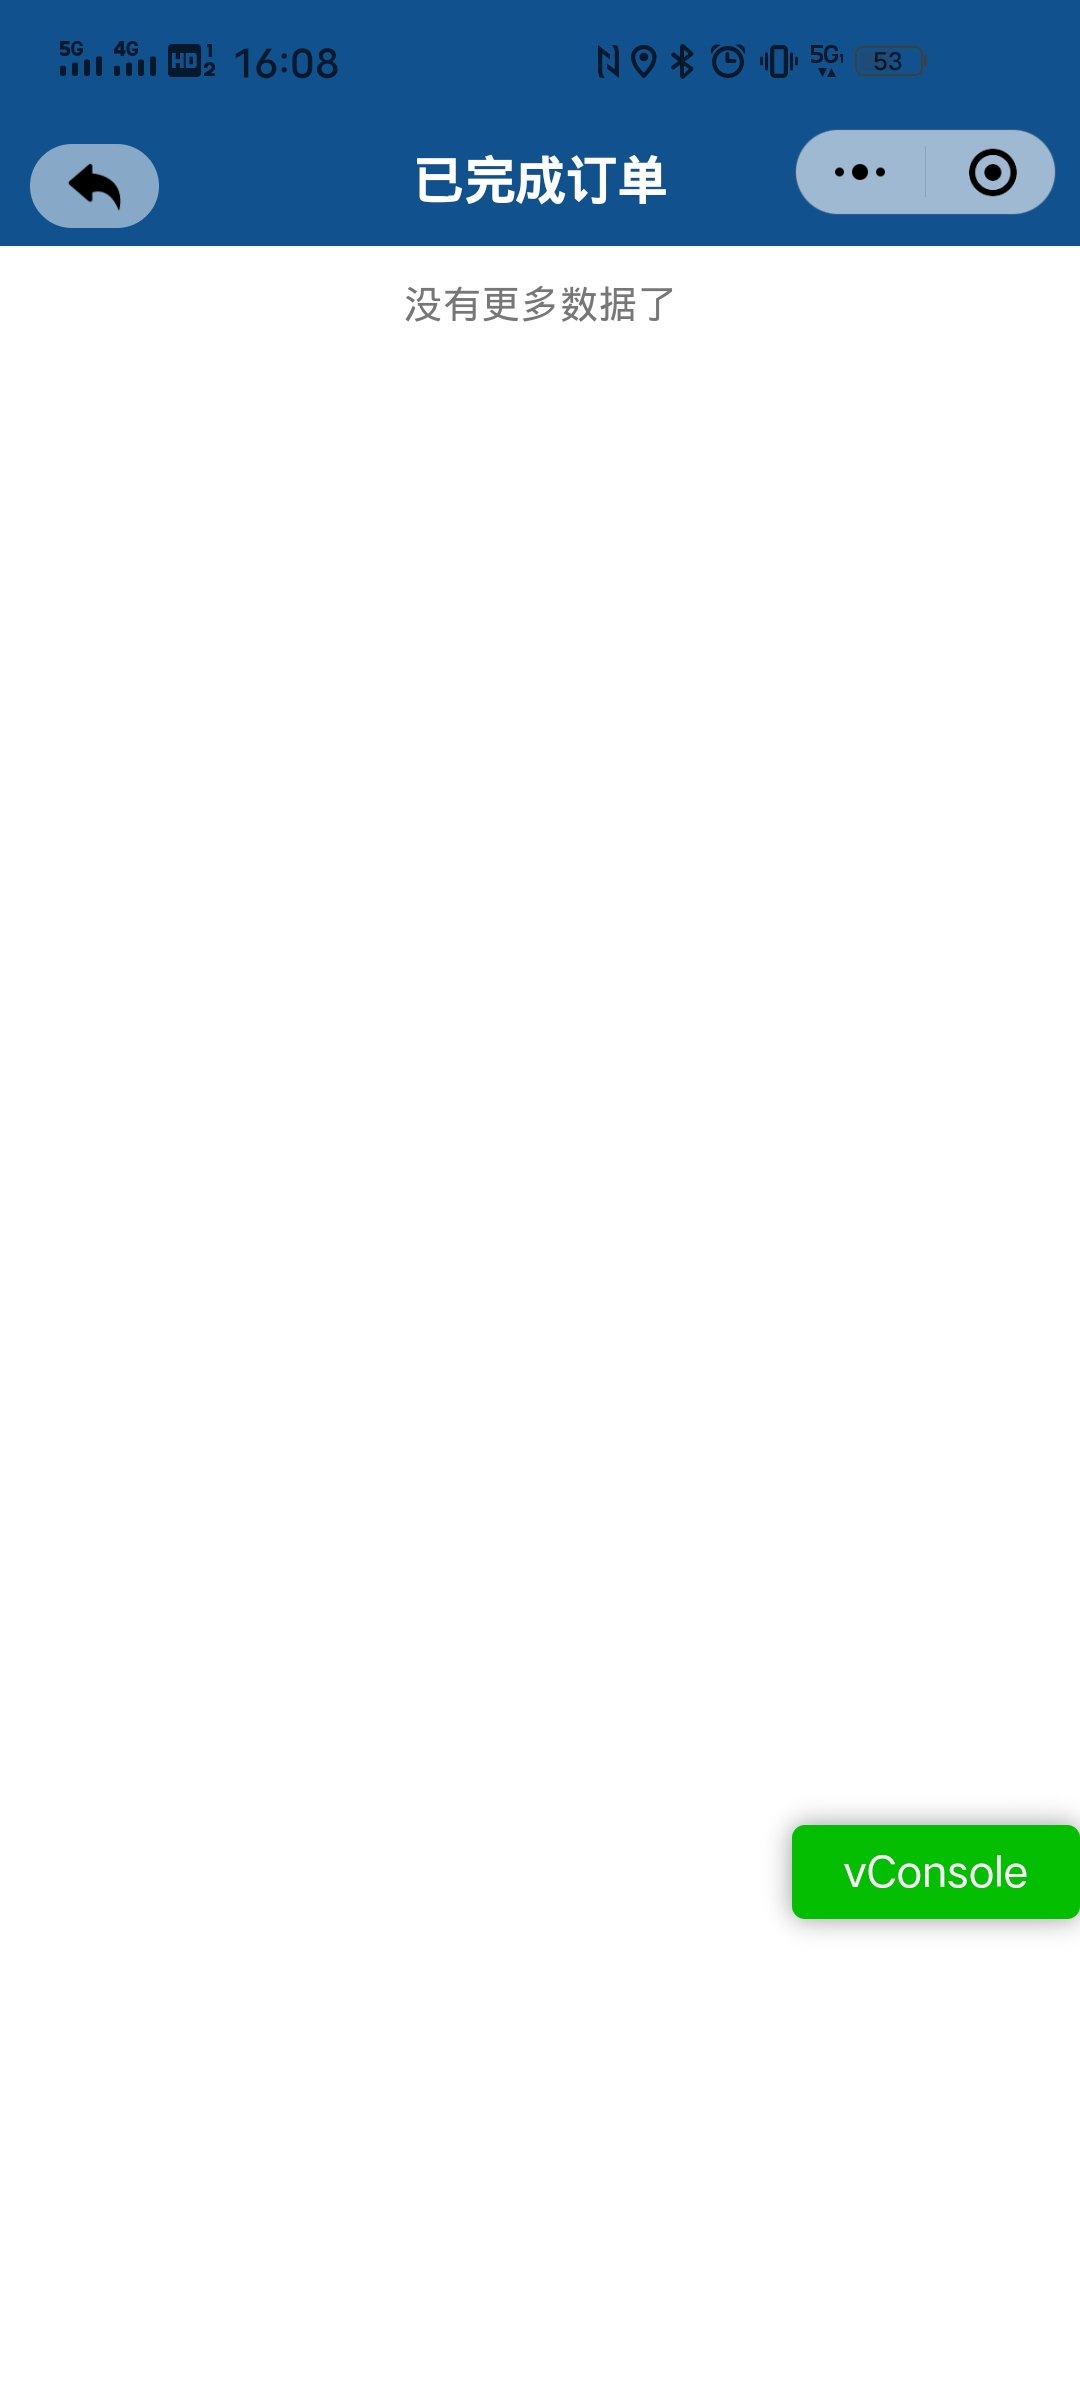
\includegraphics[height=16.0cm,width=8.0cm]{design/image/ui8.png} 
    \end{figure}
\newpage    
\section{查看 地图}

\subsection{功能说明}
用户可以在首页点击地图进入地图模式,在地图中查看出租出售的房屋位置信息
\subsection{界面设计}
\begin{figure}[htbp]
    \centering
    \begin{minipage}[t]{0.48\textwidth}
    \centering
    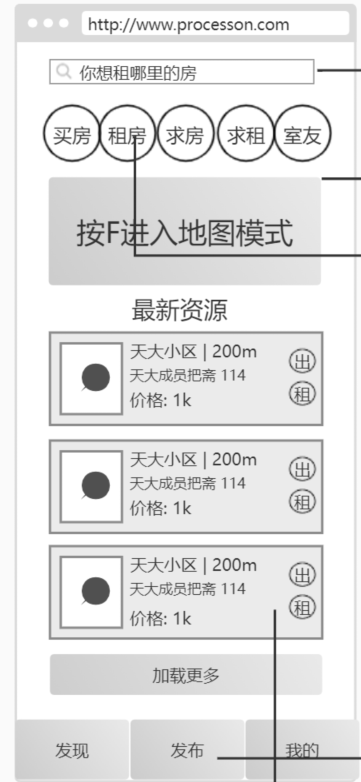
\includegraphics[width=6cm,height=13cm]{design/image/zhuye.png} 
    \caption{主页}
    \end{minipage}
    \begin{minipage}[t]{0.48\textwidth}
    \centering
    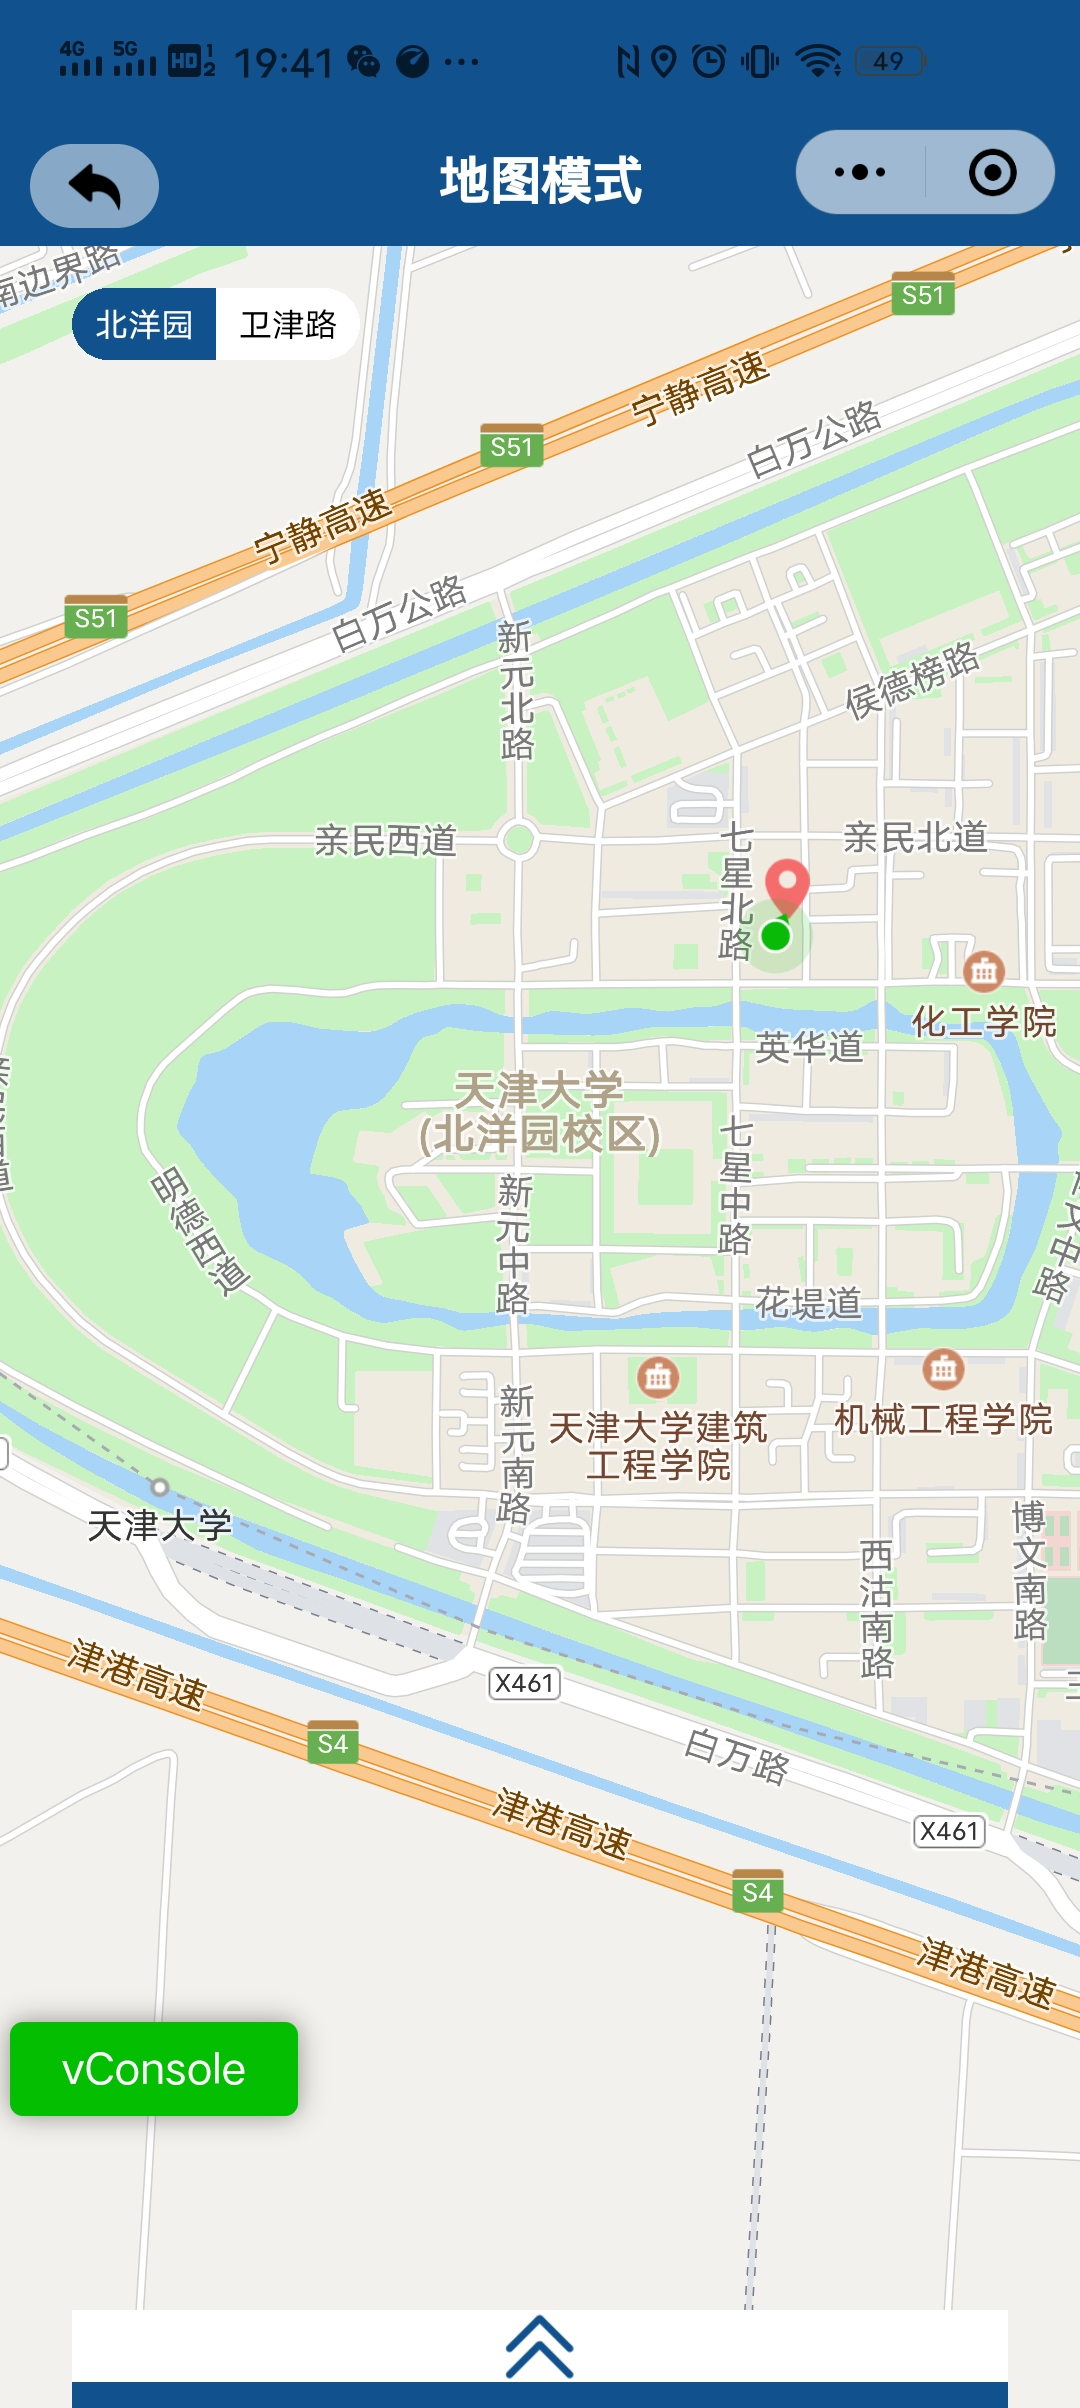
\includegraphics[width=6cm,height=13cm]{design/image/ditu2.png}
    \caption{地图}
    \end{minipage}
    \end{figure}

\newpage
\section{发布 出租帖子}

\subsection{功能说明}
用户打开发布界面,点击 我要出租.
房主填写帖子信息然后发布出租帖子
\subsection{界面设计}
\begin{figure}[htbp]
    \centering
    \begin{minipage}[t]{0.48\textwidth}
    \centering
    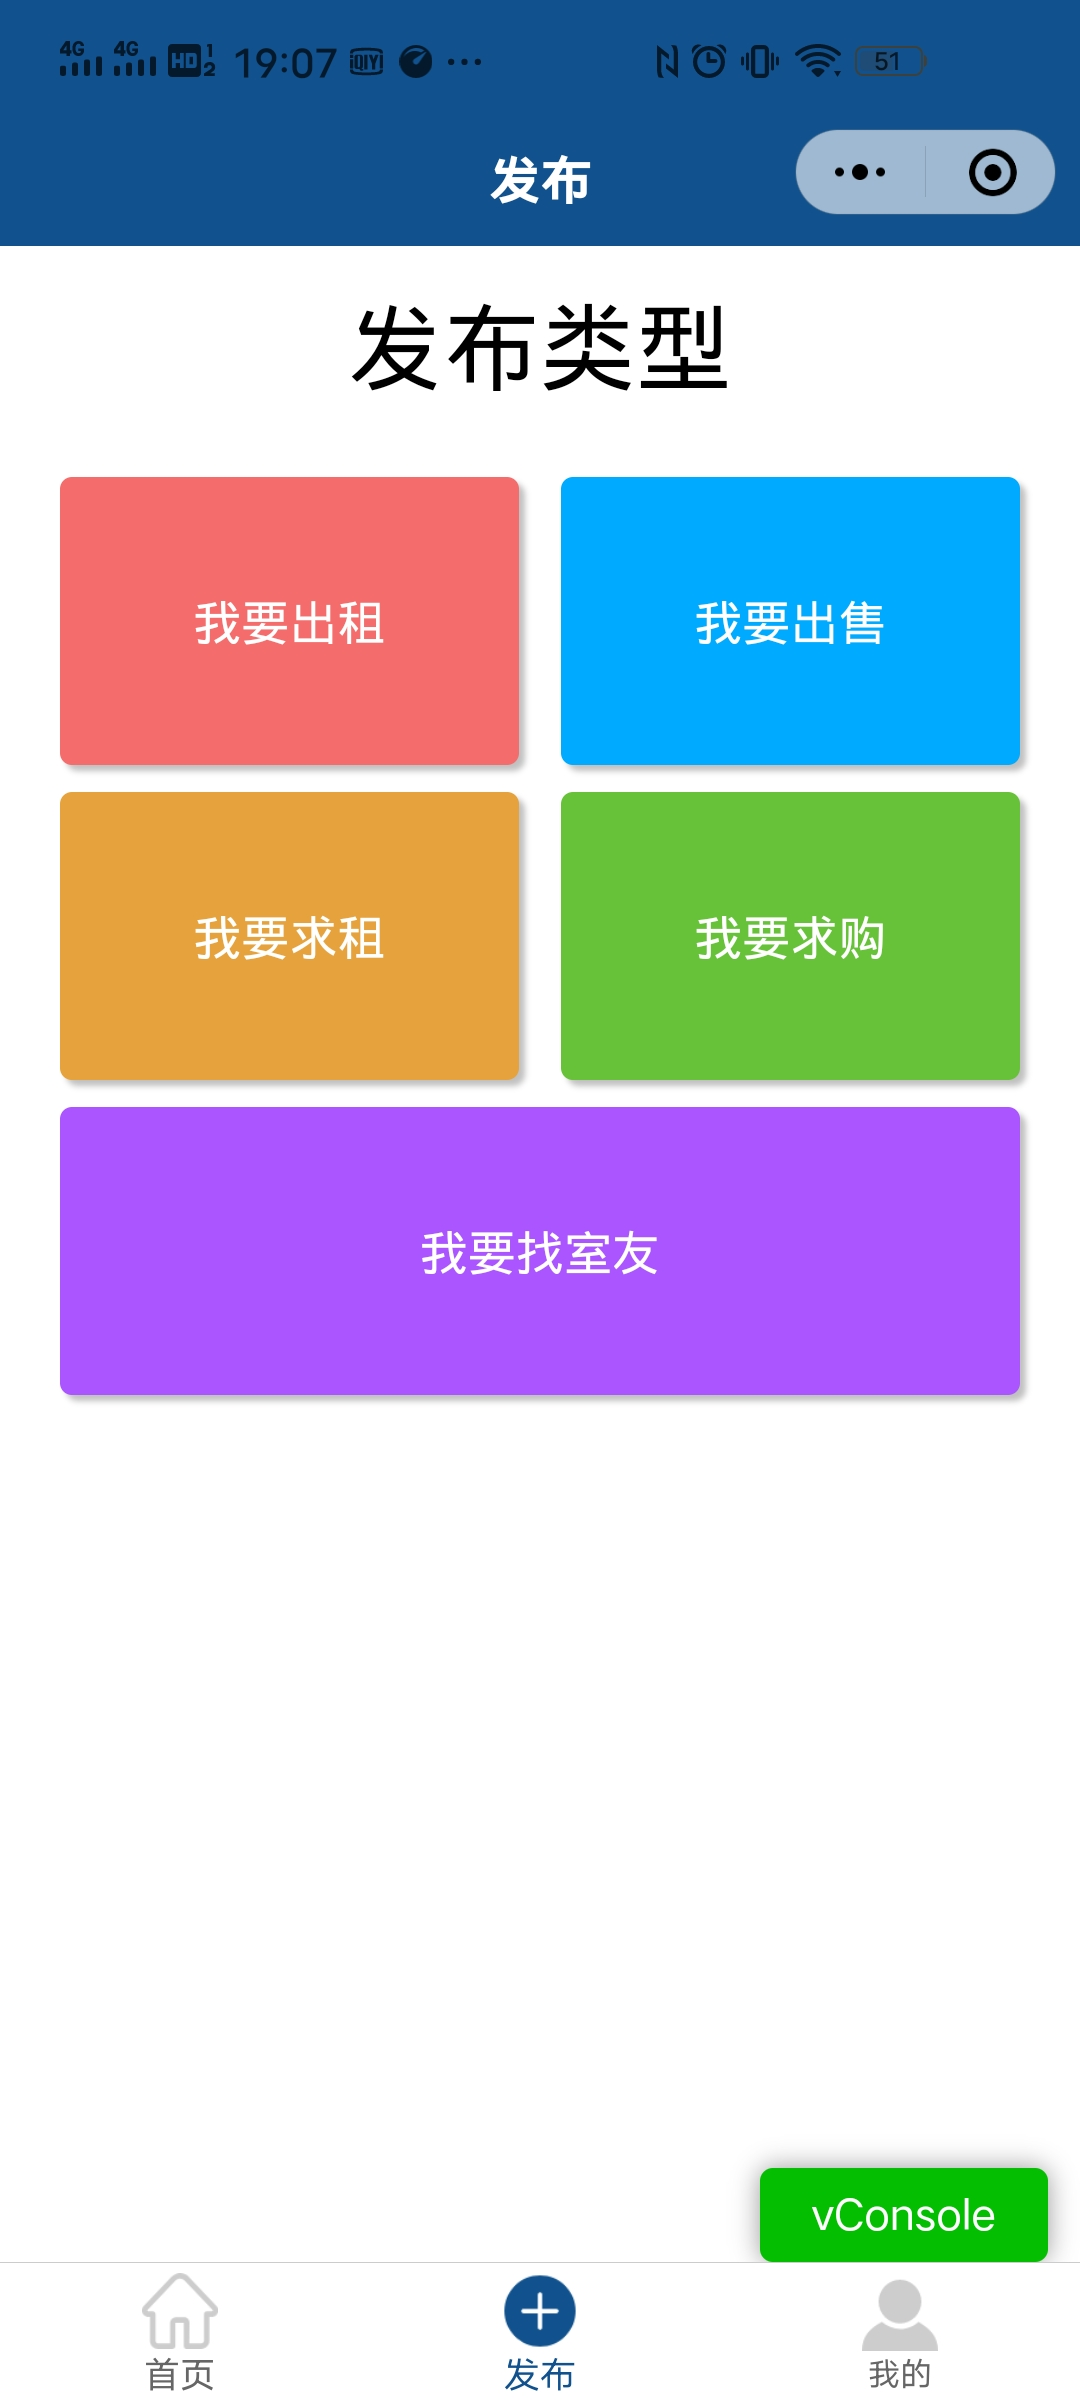
\includegraphics[width=6cm,height=13cm]{design/image/fabu0.png} 
    \caption{发布界面}
    \end{minipage}
    \begin{minipage}[t]{0.48\textwidth}
    \centering
    \includegraphics[width=6cm,height=13cm]{design/image/fabu1.png}
    \caption{发布帖子}
    \end{minipage}
    \end{figure}

\newpage
\section{发布 出售帖子}

\subsection{功能说明}
房主可以发布出售帖,出售房屋
\subsection{界面设计}

\begin{figure}[htbp]
    \centering
    \begin{minipage}[t]{0.48\textwidth}
    \centering
    \includegraphics[width=6cm,height=13cm]{design/image/fabu2.png} 
    \caption{出售帖子}
    \end{minipage}
    \begin{minipage}[t]{0.48\textwidth}
    \centering
    \includegraphics[width=6cm,height=13cm]{design/image/fabu3.png}
    \caption{求租帖子}
    \end{minipage}
    \end{figure}

\section{发布 求租帖子}

\subsection{功能说明}
用户可以发布求租帖
\subsection{界面设计}
见右上图
\newpage
\section{发布 求购帖子}

\subsection{功能说明}
用户发布求购帖
\subsection{界面设计}
\begin{figure}[htbp]
    \centering
    \begin{minipage}[t]{0.48\textwidth}
    \centering
    \includegraphics[width=6cm,height=13cm]{design/image/fabu4.png} 
    \caption{发布界面}
    \end{minipage}
    \begin{minipage}[t]{0.48\textwidth}
    \centering
    \includegraphics[width=6cm,height=13cm]{design/image/fabu5.png}
    \caption{发布帖子}
    \end{minipage}
    \end{figure}


\section{发布 找室友帖子}

\subsection{功能说明}
用户发布找室友帖子
\subsection{界面设计}
见右上图
\newpage

\section{编辑我的信息}

\subsection{功能说明}
用户打开我的界面,点击编辑信息,进行信息编辑
\subsection{界面设计}
\begin{figure}[htbp]
    \centering
    \begin{minipage}[t]{0.48\textwidth}
    \centering
    \includegraphics[width=6cm,height=13cm]{design/image/ui8.png} 
    \caption{我的界面}
    \end{minipage}
    \begin{minipage}[t]{0.48\textwidth}
    \centering
    \includegraphics[width=6cm,height=13cm]{design/image/bianji.png}
    \caption{编辑界面}
    \end{minipage}
    \end{figure}

\newpage


\section{查看已完成订单和未完成订单}
\subsection{功能说明}
用户查看已完成的订单
\subsection{界面设计}
\begin{figure}[htbp]
    \centering
    \begin{minipage}[t]{0.48\textwidth}
    \centering
    \includegraphics[width=6cm,height=13cm]{design/image/ui8.png} 
    \caption{已完成订单}
    \end{minipage}
    \begin{minipage}[t]{0.48\textwidth}
    \centering
    \includegraphics[width=6cm,height=13cm]{design/image/ui.png}
    \caption{未完成订单}
    \end{minipage}
    \end{figure}

\newpage

\section{查看消息队列}

\subsection{功能说明}
查看消息队列,点击消息队列跳转到对应的帖子的详情页
\subsection{界面设计}
\begin{figure}[htbp]
    \centering
    \begin{minipage}[t]{0.48\textwidth}
    \centering
    \includegraphics[width=6cm,height=13cm]{design/image/ui8.png} 
    \caption{消息队列}
    \end{minipage}
    \begin{minipage}[t]{0.48\textwidth}
    \centering
    \includegraphics[width=6cm,height=13cm]{design/image/xiaoxi.png}
    \caption{详情页}
    \end{minipage}
    \end{figure}

\newpage
 

\section{查看 帖子详细信息}

\subsection{功能说明}
用户查看帖子详情信息
\subsection{界面设计}
\begin{figure}[htbp]
    \centering
    \begin{minipage}[t]{0.48\textwidth}
    \centering
    \includegraphics[width=6cm,height=13cm]{design/image/xiangqing.png} 
    \caption{详情页1}
    \end{minipage}
    \begin{minipage}[t]{0.48\textwidth}
    \centering
    \includegraphics[width=6cm,height=13cm]{design/image/ui5.png}
    \caption{详情页2}
    \end{minipage}
    \end{figure}

\newpage
\section{搜索}

\subsection{功能说明}
用户进行关键字搜索,搜索想要的房屋
\subsection{界面设计}
\begin{figure}[htbp]
    \centering
    \begin{minipage}[t]{0.48\textwidth}
    \centering
    \includegraphics[width=6cm,height=13cm]{design/image/sousuo.png} 
    \caption{搜索1}
    \end{minipage}
    \begin{minipage}[t]{0.48\textwidth}
    \centering
    \includegraphics[width=6cm,height=13cm]{design/image/ui3.png}
    \caption{搜索2}
    \end{minipage}
    \end{figure}
\newpage
\section{合租}

\subsection{功能说明}
用户可以创建合租队伍,也可以加入合租队伍
\subsection{界面设计}
\begin{figure}[htbp]
    \centering
    \begin{minipage}[t]{0.48\textwidth}
    \centering
    \includegraphics[width=6cm,height=10cm]{design/image/ui9.png} 
    \caption{}
    \end{minipage}
    \begin{minipage}[t]{0.48\textwidth}
    \centering
    \includegraphics[width=6cm,height=8cm]{design/image/ui6.png}
    \caption{加入合租队伍}
    \end{minipage}
    \end{figure}
\newpage

\section{手机验证}

\subsection{功能说明}
用户绑定手机号
\subsection{界面设计}
\begin{figure}[h]
    \centering 
    \includegraphics[width=10.0cm,height=15.0cm]{design/image/check.png} 
    \end{figure}
\newpage

\newpage

\section{管理员登陆}

\subsection{功能说明}
管理员登陆
\subsection{界面设计}
\begin{figure}[h]
    \centering 
    \includegraphics[width=14.0cm,height=8.0cm]{design/image/gly.png} 
    \end{figure}
\newpage

\section{管理员用户界面}

\subsection{功能说明}
管理员管理用户信息
\subsection{界面设计}
\begin{figure}[h]
    \centering
    \includegraphics[width=14.0cm,height=8.0cm]{design/image/usergl.png} 
    \end{figure}
\newpage

\section{管理员帖子管理界面}

\subsection{功能说明}
管理员管理帖子信息
\subsection{界面设计}

\begin{figure}[h]
    \centering
    \includegraphics[width=14.0cm,height=8.0cm]{design/image/tiezigl.png} 
    \end{figure}
\newpage


    
	 
	% \clearpage

\end{CJK*}                                     % 结束中文字体使用
\end{document}                                 % 结束全文
